

%\documentclass[pra,twocolumn,epsfig,rotate,superscriptaddress,showpacs]{revtex4}


% \mathcal{u}se only LaTeX2e, calling the article.cls class and 12-point type.

\documentclass[prl,onecolumn]{revtex4-1}
\usepackage{graphicx}
\usepackage{epsfig}
\usepackage{epsf}
\usepackage{amssymb}
\usepackage{amsmath}
\usepackage{amsthm}
\usepackage{multirow}
\usepackage[colorlinks,linkcolor=red,anchorcolor=blue,citecolor=green]{hyperref}

\usepackage{graphicx}
\usepackage{subfigure}
\usepackage{color}

\graphicspath{{Figures/}}
\includeonly{main,Appendix3}
% Appendix, Appendix2, Appendix3


\usepackage{tabu} % table macro

\usepackage[framed,numbered]{matlab-prettifier}
\let\ph\snippetPlaceholder
\lstset
{
  style = Matlab-editor,
  escapechar      = ",
}

\renewcommand{\familydefault}{\sfdefault}  %% arial font
% \usepackage{times} %% times new roman font

\newcommand{\bra}[1]{\langle #1|}
\newcommand{\ket}[1]{|#1\rangle}
\newcommand{\dir}{$\backslash$}
\newcommand{\be}{\begin{equation}}
\newcommand{\ee}{\end{equation}}
\newcommand{\bea}{\begin{eqnarray}}
\newcommand{\eea}{\end{eqnarray}}
\newcommand{\Fig}[1]{Fig.\,\ref{#1}}
\newcommand{\Eq}[1]{Eq.\,(\ref{#1})}
\newcommand{\la}{\langle}
\newcommand{\ra}{\rangle}
\newcommand{\nl}{\nonumber \\}
%\usepackage[usenames]{color}
%\definecolor{Red}{rgb}{1,0,0}
%\definecolor{Blue}{rgb}{0,0,1}




\setlength{\parindent}{0pt} % no incident
%\renewcommand{\baselinestretch}{1.2} % space between two lines
\setlength{\parskip}{6\lineskip} % space between two paragraphs

%%%%%%%%%%%%%%%%% END OF PREAMBLE %%%%%%%%%%%%%%%%



\begin{document}

% Include your paper's title here
\title{Notes on the 12 qubit PPS}
\author{Dawei Lu}

\begin{abstract}
Notes about the problems in the 12 qubit PPS preparation, including Matlab codes and Experiments.
\end{abstract}
\today

\maketitle

\section{Dec 12-Feb 06, 2014: GRAPE Pulse Calculations and Simulations}

{\color{blue}{\textbf{Dec 12, 2014:}}}

\textbf{I tried state to state GRAPE pulses. The one to evolve ZZZZZZZIIIII to ZZZZZZZZZZZZ cannot be found, but the C-H SWAP gate can.}

Calculating the state to state GRAPE on Ordi2. In pulsefinder folder. paramsfile is 'twqubit\_subS2S.m', and the output file is 'twqubit\_7zto12z'.

The GRAPE is to evolve ZZZZZZZIIIII to ZZZZZZZZZZZZ. As the couplings between nearest-neighbored C and H are about 150Hz. I set the GRAPE as 4ms and 400 steps, with Zfreedom allowed.

The fidelity keeps 0 all the time. Guess the reason is 'Zfreedom'. Set 'params.Zfreedomflag = 0;'. However, still 0.

Annie said maybe due to the length. Her SWAP gate requires 8ms, so I changed 'params.plength = 800;'. But for with or without Zfreedom, fidelity is still 0.

Check if some of my GRAPE settings are wrong. try to repeat Annie's SWAP gate calculation.

\begin{lstlisting}
% Number of timesteps
params.plength = 800;

% Length of each time step
params.timestep = 10e-6;

params.subsystem{1} = [1 2 3 9 10 11];
params.subsystem{2} = [4 5 6 7 8 12];
params.subsys_weight = [6 6];

% Input and goal states for state to state
params.rhoin = mkstate('+1IIIIIIIZIIII+1IIIIIIIIZIII+1IIIIIIIIIZII+1IIIIIIIIIIZI+1IIIIIIIIIIIZ',1);
params.rhogoal = mkstate('+1IIIIIIIZIIII+1IIIIIIIIZIII+1IIIIIIIIIZII+1IIIIIIIIIIZI+1IIIIIIZIIIIZ',1);

% Allow Zfreedom or not
params.Zfreedomflag = 0;
\end{lstlisting}

The outputfile is 'twqubit\_SWAPC7H5'. And the fidelity is already over 98\%. Then I changed 'params.Zfreedomflag = 1;', and the fidelity is over 95\% after 30 iterations. Much slower than the no Zfreedom case. Maybe due to different initial guesses.

{\color{blue}{\textbf{Dec 15, 2014 to Mar 03, 2015:}}}

\textbf{All single qubit $\pi/2$ and $\pi$ have been generated by the sub-system method. The fidelity and unitary operator of each pulse in the whole system is also calculated.}

Generate all $\pi/2$ and $\pi$ pulses for the 7 Carbons, with the Calibration = 25KHz. $\pi/2$ pulses are 1ms length and 100 steps, and $\pi$ pulses are 2ms length and 200 steps. Generating Code in 'twqubit\_shape.m'

\begin{lstlisting}
for ii = 1:7
loadfile = ['twqubit_C', num2str(ii), '180', '.mat'];
eval(['load ', loadfile]);
filename1 = ['twqubit_C', num2str(ii), '180_C_25000.txt'];
filename2 = ['twqubit_C', num2str(ii), '180_H_25000.txt'];
make_bruker_shape(pulses{1}, 25000, filename1,1);
make_bruker_shape(pulses{1}, 25000, filename2,2);
end
\end{lstlisting}

To generate $\pi$ pulses, In the beginning, I wanted to combine two $\pi/2$ pulses. A potential problem is when calculating the GRAPE, we have considered the 4us free evolutions in the beginning and in the end. If we combine, we will have an unwanted 8us free evolution in the middle of the new $\pi$ pulse. So I used 'combine90to180' to check the $\pi$ pulse fidelity. They are very bad actually. All of them are just 0.75~0.76 in fidelity. However, we can still use them as the initial guess to search the optimal $\pi$ pulse. By using them, the convergence speed is very fast, which means the initial guess is indeed very important in 12 qubits.

The pulses are saved in Ordi2 '\dir pulsefinder\dir 12 Qubit\dir' with the names such as 'twqubit\_C590\_C\_25000.txt'. After that,
I checked all the fidelities of the pulses in the folder '\dir pulseexam\_12qubit\dir C\_rotations\dir check\_grape.m'. The code is in \hyperlink{code:check_grape}{Appendix I}. To my surprise, all fidelities in the 12-qubit system are still over 0.99, which means the separation of the two sub-systems are pretty well.

Unitaries and Fidelities of the pulses will both be saved in 'twqubit\_C590\_Ufid.mat', so they can be called for further calculations in the PPS simulation. The folder is '\dir pulseexam\_12qubit\dir C\_rotations\dir'. Use 'check\_power.m' to check the maximal powers for C and H channel to guarantee all powers are within the power limit. For details, see the Table below\ref{all_single_pulses}.

\begin{table}[hbtp]
\begin{tabular} {c||c|c|c|c|c}
  \hline
  Rotation & Length & Fidelity & File & MaxPower C & MaxPower H\\
  \hline
  % after \\: \hline or \cline{col1-col2} \cline{col3-col4} ...
  $R_x^1(\pi/2)$ & 1ms & 0.9981 & twqubit\_C190\_Ufid.mat & 56.0\%, 14000Hz & 22.3\%, 5557Hz\\
  $R_x^2(\pi/2)$ & 1ms & 0.9986 & twqubit\_C290\_Ufid.mat & 41.7\%, 10422Hz & 23.5\%, 5878Hz\\
  $R_x^3(\pi/2)$ & 1ms & 0.9981 & twqubit\_C390\_Ufid.mat & 31.9\%, 7979.0Hz & 22.3\%, 5568Hz\\
  $R_x^4(\pi/2)$ & 1ms & 0.9976 & twqubit\_C490\_Ufid.mat & 31.6\%, 7892.0Hz & 23.8\%, 5954Hz\\
  $R_x^5(\pi/2)$ & 1ms & 0.9981 & twqubit\_C590\_Ufid.mat & 56.1\%, 14033Hz & 30.7\%, 7678Hz\\
  $R_x^6(\pi/2)$ & 1ms & 0.9979 & twqubit\_C690\_Ufid.mat & 57.3\%, 14333Hz & 34.4\%, 8595Hz\\
  $R_x^7(\pi/2)$ & 1ms & 0.9986 & twqubit\_C790\_Ufid.mat & 43.7\%, 10925Hz & 24.8\%, 6207Hz\\
  \hline
  \hline
  $R_x^1(\pi)$ & 2ms & 0.9976 & twqubit\_C1180\_Ufid.mat & 62.6\%, 15655Hz & 34.9\%, 8726Hz\\
  $R_x^2(\pi)$ & 2ms & 0.9980 & twqubit\_C2180\_Ufid.mat & 51.1\%, 12783Hz & 32.4\%, 8094Hz\\
  $R_x^3(\pi)$ & 2ms & 0.9975 & twqubit\_C3180\_Ufid.mat & 37.4\%, 9350.0Hz & 24.0\%, 5997Hz\\
  $R_x^4(\pi)$ & 2ms & 0.9970 & twqubit\_C4180\_Ufid.mat & 45.1\%, 11268Hz & 20.4\%, 5108Hz\\
  $R_x^5(\pi)$ & 2ms & 0.9975 & twqubit\_C5180\_Ufid.mat & 67.6\%, 16895Hz & 31.1\%, 7782Hz\\
  $R_x^6(\pi)$ & 2ms & 0.9976 & twqubit\_C6180\_Ufid.mat & 71.8\%, 17948Hz & 33.6\%, 8396Hz\\
  $R_x^7(\pi)$ & 2ms & 0.9977 & twqubit\_C7180\_Ufid.mat & 51.0\%, 12759Hz & 32.1\%, 8022Hz\\
  \hline
\end{tabular}\label{all_single_pulses}
\end{table}

{\color{blue}{\textbf{Dec 22, 2014 to Feb 06, 2015:}}}

\textbf{Got all the 5 GRAPE pulses for encoding. }The folder is '\dir pulseexam\_12qubit\dir C\_rotations\dir'. Here is the Table listing all the details of the 5 encoding pulses.

\begin{table}[hbtp]
\begin{tabular} {c||c|c|c|c|c}
  \hline
  Rotation & Length & Fidelity & File & MaxPower C & MaxPower H\\
  \hline
  % after \\: \hline or \cline{col1-col2} \cline{col3-col4} ...
  $R_x^{5,7}(\pi)$ & 2ms & 0.9980 & twqubit\_C57180\_Ufid.mat & 32.3\%, 8072.5Hz & 24.2\%, 6049Hz\\
  $R_x^{2,3}(\pi)$ & 2ms & 0.9978 & twqubit\_C23180\_Ufid.mat & 32.4\%, 8101.5Hz & 22.8\%, 5701Hz\\
  $R_x^{2,3,4,7}(\pi/2)$ & 1ms & 0.9970 & twqubit\_C234790\_Ufid.mat & 37.4\%, 9358.3Hz & 28.9\%, 7213Hz\\
  $R_x^{1,5,6}(\pi)$ & 2ms & 0.9974 & twqubit\_C156180\_Ufid.mat & 32.2\%, 8039.7Hz & 20.3\%, 5086Hz\\
  $R_x^{2,4,7}(\pi/2)R_{-y}^{3}(\pi/2)R_{-z}^{i=2,3,4,7}((w_i-O_1)*3.36\text{ms})$ & 1ms & 0.9964 & twqubit\_C234790withPC\_Ufid.mat & 26.1\%, 6514.5Hz & 20.2\%, 5048Hz\\
  \hline
\end{tabular}
\end{table}

The last pulse for the Encoding is (From the PPS.m file in folder 'Twqubit')
\begin{lstlisting}
%Phase Correction
U7 = R(gop(2,X),90)*R(gop(2,-Z),360*(Para(2,2)-20696)*1/2/148.5)*...
R(gop(3,-Y),90)*R(gop(3,-Z),360*(Para(3,3)-20696)*1/2/148.5)*...
R(gop(4,X),90)*R(gop(4,-Z),360*(Para(4,4)-20696)*1/2/148.5)*...
R(gop(7,X),90)*R(gop(7,-Z),360*(Para(7,7)-20696)*1/2/148.5);
\end{lstlisting}


%And the operator is in 'twqubit\_sub\_234790\_and\_phasecorrection.m'
%\begin{lstlisting}
%params.Uwant = expm(-1i*(90*pi/180)/2*full(mkstate('+1IXIIIIIIIIII-1IIYIIIIIIIII+1IIIXIIIIIIII+1IIIIIIXIIIII',0)))*...
%expm(-1i*((8778.95-20696)*1/2/148.5*360*pi/180)/2*full(mkstate('-1IZIIIIIIIIII',0)))*...
%expm(-1i*((6245.16675-20696)*1/2/148.5*360*pi/180)/2*full(mkstate('-1IIZIIIIIIIII',0)))*...
%expm(-1i*((10333.55-20696)*1/2/148.5*360*pi/180)/2*full(mkstate('-1IIIZIIIIIIII',0)))*...
%expm(-1i*((11928.21998-20696)*1/2/148.5*360*pi/180)/2*full(mkstate('-1IIIIIIZIIIII',0)));
%\end{lstlisting}

\clearpage
{\color{blue}{\textbf{Feb 18, 2014:}}}

\textbf{Got two pulses for phase cycling and polarization crush. }One is 'twqubit\_all90.m' which is used for phase cycling, and the other one is 'twqubit\_all90butC7.m' used for the polarization crush in the beginning.
\begin{table}[hbtp]
\begin{tabular} {c||c|c|c|c|c}
  \hline
  Rotation & Length & Fidelity & File & MaxPower C & MaxPower H\\
  \hline
  % after \\: \hline or \cline{col1-col2} \cline{col3-col4} ...
  $R_x^{1-12}(\pi/2)$ & 1ms & 0.9977 & twqubit\_all90\_Ufid.mat & 27.8\%, 6956.6Hz & 30.4\%, 7594Hz\\
  $R_x^{1-6,8-12}(\pi/2)$ & 1ms & 0.9977 & twqubit\_all90butC7\_Ufid.mat & 24.5\%, 6134.9Hz & 25.0\%, 6239Hz\\
  \hline
\end{tabular}
\end{table}

{\color{blue}{\textbf{Mar 03, 2014:}}}

\textbf{All 6 pulses for the decoding part have been checked.}

\begin{table}[!h]
\begin{tabular} {c||c|c|c|c|c}
  \hline
  Rotation & Length & Fidelity & File & MaxPower C & MaxPower H\\
  \hline
  % after \\: \hline or \cline{col1-col2} \cline{col3-col4} ...
  $R_x^{2,3,4,7-12}(\pi)$ & 2ms & 0.9988 & twqubit\_C2347andH180\_Ufid.mat & 61.6\%, 15400Hz & 52.2\%, 13039Hz\\
  $R_x^{1,3,4,6}(\pi/2)R_{-y}^{8-12}(\pi/2)$ & 1ms & 0.9974 & twqubit\_C134690andH90\_Ufid.mat & 24.8\%, 6203.2Hz & 22.1\%, 5529Hz\\
  $R_x^{2,3,4,5,6}(\pi)$ & 2ms & 0.9984 & twqubit\_C23456180\_Ufid.mat & 37.8\%, 9438.2Hz & 23.0\%, 5746Hz\\
  $R_{-y}^{4,6}R_{y}^{1,3}(\pi/2)R_{x}^{2}(\pi/2)R_{-z}^{1}(6.6\text{ms})$ & 1ms & 0.9982 &  twqubit\_C1234690withPC\_Ufid.mat & 28.3\%, 7070.8Hz & 26.9\%, 6717Hz\\
  $R_x^{2,7}(\pi)$ & 2ms & 0.9979 & twqubit\_C27180\_Ufid.mat & 29.1\%, 7285.3Hz & 21.7\%, 5414Hz\\
  $R_{y}^{2}(\pi/2)R_{x}^{5}(\pi/2)$ & 1ms & 0.9975 & twqubit\_C2Y5X90\_Ufid.mat & 28.9\%, 7233.9Hz & 29.2\%, 7292Hz\\
  \hline
\end{tabular}
\end{table}

\clearpage
\section{May 09, 2015 to May 10, 2015: Recalculation of GRAPE pulses with 0us Buffer}

{\color{blue}{\textbf{Mar 09, 2015:}}}

\hypertarget{reason:pulse_no_buffer}{The reason of this recalculation is described}
\hyperlink{found:pulse_no_buffer}{here}.

According to the fact that 4us cannot be absorbed into a 10us shape pulse, I decided to delete the buffer delay in the GRAPE calculation. An AU program called 'GRAPE\_recal\_nobuffer.m' was written to do it. The directory in Ordi2 is '\dir pulseexam\_12qubit\dir C\_rotations\dir GRAPE\_nobuffer\dir' or in the SVN '\dir Matlab\dir Twqubit\dir Pulse\_NoBuffer\dir'.

There are 18 pulses required for recalculation with 8 $\pi/2$ rotations and 10 $\pi$ rotations. In the program, I first regenerate Bx and By from the shaped pulses, and use them as the initial guess, saved in files titled like 'twqubit\_C190\_InitialGuess.mat'. Then generate the params setting file with 0us buffer. \textbf{Note the power limit of C channel is set as 12.5KHz instead of 25KHz. }Both the initial guess file and params setting file are transferred to Feynman and Ordi2 by the scp command. A cluster sample is also written and saved in Ordi2 pulsefinder folder.

In calculation on Feynman in the weekend. All the 18 pulses
\begin{lstlisting}
Pulse_Name{1} = 'twqubit_C790';
Pulse_Name{2} = 'twqubit_C290';
Pulse_Name{3} = 'twqubit_C234790';
Pulse_Name{4} = 'twqubit_C234790withPC';
Pulse_Name{5} = 'twqubit_C134690andH90';
Pulse_Name{6} = 'twqubit_C1234690withPC';
Pulse_Name{7} = 'twqubit_C2Y5X90';
Pulse_Name{8} = 'twqubit_C590';
Pulse_Name{9} = 'twqubit_C2180';
Pulse_Name{10} = 'twqubit_C6180';
Pulse_Name{11} = 'twqubit_C4180';
Pulse_Name{12} = 'twqubit_C57180';
Pulse_Name{13} = 'twqubit_C1180';
Pulse_Name{14} = 'twqubit_C23180';
Pulse_Name{15} = 'twqubit_C156180';
Pulse_Name{16} = 'twqubit_C2347andH180';
Pulse_Name{17} = 'twqubit_C23456180';
Pulse_Name{18} = 'twqubit_C27180';
\end{lstlisting}

Got almost all pulses with fidelity over 0.995. The exception is pulse Number 10, C6180. The reason should be the power limit 12.5KHz is not enough. So change it to 25KHz again and recalculate this GRAPE. All the GRAPE .mat files are transferred to '\dir Matlab\dir Twqubit\dir Pulse\_NoBuffer\dir'.

An AU program 'make\_shape\_12qubit.m' for making the Bruker shape is used to generate all Burker files. Then the maximal power is checked using 'check\_power\_NoBuffer.m'. The powers are almost the same as the ones from the initial guess, and \textbf{are updated everywhere in this draft}.

\clearpage
\section{Dec 16, 2014 to Feb 12, 2015: Combining GRAPE Pulses to Big Shape Files}

{\color{blue}{\textbf{Dec 16, 2014:}}}

Combine pulses in the PPS preparation into big shape files, which should be easy for calibrations and pulsefixing. \textbf{Note later I fixed each pulse independently and combine the fixed ones together, as the optimal fix number for each pulse can be different.}

The code is in the SVN server for Matlab named '\dir Twqubit\dir pulse\_combine.m'.

First read all the powers and phases for the $\pi/2$ and $\pi$ rotations. The code is in \hyperlink{code:read_power_phase}{Appendix I}.

Then combine them with the free evolutions. Here I set the time step dt = 10us. The code is in \hyperlink{code:combine_encoding1}{Appendix I}.

The two output files are 'twqubit\_encoding1\_C' and 'twqubit\_encoding1\_H'. The calibrations are 25000Hz.

{\color{blue}{\textbf{Feb 12, 2015:}}}

\textbf{Solved the problem that how to change the phase of GRAPE pulses to other phases. For example, if we already have a X rotation, how can we rewrite the phase column to make it realize a Y rotation.}

When combining all pulses into a large shape file, one has to know how to change a shape for X rotation to Y rotation. It should be a $\pi/2$ phase difference for every segment in the shape. I am going to check it.

The checking uses 4-qubit Crotonic in the folder 'F:\dir matlab\dir pulseexam\_7qubit\dir 4 qubit pulse check'. The target unitary is $R_x^1(\pi/2)$, and the pulse is 'Croton\_90x1.txt' with length 1ms, 500 segments and amplitude 6000Hz.

When compared with $R_x^1(\pi/2)$, the fidelity is 0.9996. Then I changed the target to $R_y^1(\pi/2)$ with the GRAPE pulse unchanged. The fidelity goes to 0.4998 which is reasonable.

In order to produce a $R_y^1(\pi/2)$ from the original X rotation pulse, I added 90 to all phases in all segments. However, the fidelity goes to almost 0. Again all phases are reduced by 90, and this time the fidelity is 0.9996, which is what we want!

Conclusion: If you want to realize a Y rotation based on a X rotation pulse, just change the phase to phase-90 in each segment, and mod by 360 for the spectrometer.
\begin{lstlisting}
phase = phase - 90;
phase = mod(phase, 360);
\end{lstlisting}
I wrote a program 'grape\_phase' to generate the new phase in the folder 'F:\dir matlab\dir pulseexam\_7qubit\dir'. Used in this manner  'phase\_new = grape\_phase( phase, initial\_phase, end\_phase)', where the initial\_phase and end\_phase can be X, Y, -X, or -Y.

The way to get the new operator is through the equation $R_z(\theta) = XR_y(\theta)\bar{X}$. If you know the unitary $U_x$ of the X rotation pulse, and when you are realizing Y pulse from that one, the new unitary $U_y$ is thus
\be
U_y = R_z(\pi/2)U_xR_z(-\pi/2);
\ee

Generated the first encoding part, which will evolve Z7 to Z24567. The files 'twqubit\_encoding1\_C' and 'twqubit\_encoding1\_H' are in Ordi2 '\dir pulseexam\_12qubit'. The total length is 32.98ms. Next I have to check whether the final state after this pulse will be Z24567 or not. So 'check\_encoding.m' is written. The directory is Ordi2 '\dir pulseexam\_12qubit'. This function will load all necessary .mat files to get the unitaries and calculate the final state based on these unitaries from Z7.

The final fidelity is 0.9832 (the same for with or without gradient) for Z24567. Two files 'U\_encoding1.mat' and 'rho\_encoding1.mat'. Now go on to the second Encoding part.

The fidelity for the second Encoding part is -0.9692 (the same for with or without gradient) for Z1234567. Two files 'twqubit\_encoding2\_C' and 'twqubit\_encoding2\_H' are in Ordi2 '\dir pulseexam\_12qubit'. The total length is 21.29ms. Then the last piece in Encoding!

The fidelity for the third Encoding part is -0.9160 (the same for with or without gradient) for Z123456789101112. Two files 'twqubit\_encoding3\_C' and 'twqubit\_encoding3\_H' are in Ordi2 '\dir pulseexam\_12qubit'. The total length is 7.36ms.

\textbf{Update on Mar 04}: In the last code, the free evolution time is not the integer times of 10us, but it should be. So the function 'F.m' is modified as
\begin{lstlisting}
function F=F(Hamiltonian, time)
F=diag(exp(diag(-i*Hamiltonian*10e-6*round(time/10e-6))),0);
\end{lstlisting}
And all the fidelities are recalculated. They are 0.9831 for Encoding 1,  -0.9717 for Encoding 2, -0.9124 for Encoding 3.

\clearpage
\section{Mar 04, 2015: Re-Check and Simplified the PPS Circuit in Simulation}

I found the decoding part can be simplified. Check it in Matlab.

All the files are saved in Ordi2 '\dir twqubit\dir'. For the encoding which consists of three parts, the fidelities have been checked before.
\begin{table}[hbtp]
\caption{Encoding in 12-qubit PPS}
\begin{tabular} {c||c|c|c}
  \hline
  Target State & State Fidelity & Density Matrix & Unitary Operator\\
  \hline
  % after \\: \hline or \cline{col1-col2} \cline{col3-col4} ...
  IZIZZZXIIIII & 1.0000 & rho\_encoding1.mat & U\_encoding1.mat\\
  ZXZZZZZIIIII & -1.0000 & rho\_encoding2.mat & U\_encoding2.mat\\
  ZZZZZZZZZZZZ & -0.9500 & rho\_encoding3.mat & U\_encoding3.mat\\
  \hline
\end{tabular}
\end{table}

For the phase cycling it has been done too.
\begin{table}[hbtp]
\caption{Phase Cycling in 12-qubit PPS}
\begin{tabular} {c||c|c|c}
  \hline
  Target State & State Fidelity & Density Matrix & Unitary Operator\\
  \hline
  % after \\: \hline or \cline{col1-col2} \cline{col3-col4} ...
  $\ket{00...0}\bra{00...0} + \ket{11...1}\bra{11...1}$ & 0.9511 & rho\_phasecycling.mat & NAN\\
  \hline
\end{tabular}
\end{table}

For the decoding part, the simulation is as follows.
\begin{table}[hbtp]
\caption{Decoding in 12-qubit PPS}
\begin{tabular} {c||c|c|c}
  \hline
  Target State & State Fidelity & Density Matrix & Unitary Operator\\
  \hline
  % after \\: \hline or \cline{col1-col2} \cline{col3-col4} ...
  $\begin{array}{c}
     A_1A_5A_6 \ket{+---++-00000}+ \\
     A_1'A_5'A_6' \ket{-+++--+00000}
   \end{array}
  $ & 0.8717 & rho\_decoding1.mat & U\_decoding1.mat\\
  \hline
    $\begin{array}{c}
     A_1A_5A_6A_7 \ket{0+00-0-00000}+ \\
     A_1'A_5'A_6'A_7' \ket{0-00+0+00000}
   \end{array}
  $ & 0.8570 & rho\_decoding2.mat & U\_decoding2.mat\\
  \hline
  $\begin{array}{c}
     A_1A_5A_6A_7A_5^{new} \ket{000000-00000}+ \\
     A_1'A_5'A_6'A_7'A_5^{new'} \ket{000000+00000}
   \end{array}
  $ & 0.8570 & rho\_decoding3.mat & U\_decoding3.mat\\
  \hline
\end{tabular}
\end{table}

A$_1$, A$_5$ and A$_6$ are phases produced by the chemical shift evolutions of C1, C5 and C6 during $1/2\text{J}_{\text{C7H5}}$. A$_7$ is the phase by the chemical shift evolution of C7 (\textbf{Note: C7 is x-iy so the phase is the conjugate}) during $1/2\text{J}_{\text{C2C3}}$, and the coupling evolutions between C7 and all protons. A$_5^{new}$ is the phase of C5 again in $1/2\text{J}_{\text{27}}$, including the chemical shift evolution and coupling evolutions (J25 and J57 are switched off). So the phases are
\bea
A_1 & = &cos(2\pi(\omega_1-O_1)/2\text{J}_{\text{C7H5}})-isin(2\pi(\omega_1-O_1)/2\text{J}_{\text{C7H5}}), \\ \nonumber
A_5 & = &cos(2\pi(\omega_5-O_1)/2\text{J}_{\text{C7H5}})-isin(2\pi(\omega_5-O_1)/2\text{J}_{\text{C7H5}}), \\ \nonumber
A_6 & = &cos(2\pi(\omega_6-O_1)/2\text{J}_{\text{C7H5}})-isin(2\pi(\omega_6-O_1)/2\text{J}_{\text{C7H5}}), \\ \nonumber
A_7 & = &cos(2\pi(\omega_7-O_1)/2\text{J}_{\text{23}})+isin(2\pi(\omega_7-O_1)/2\text{J}_{\text{23}})* \\ \nonumber
&& \prod_{k=8}^{12} (cos(\pi\text{J}_{\text{7k}}/\text{J}_{\text{23}})+isin(\pi\text{J}_{\text{7k}}/\text{J}_{\text{23}})), \\ \nonumber
A_5^{new} & = &cos(2\pi(\omega_5-O_1)/2\text{J}_{\text{27}})+isin(2\pi(\omega_5-O_1)/2\text{J}_{\text{27}})* \\ \nonumber
&& \prod_{k\neq 2, 5, 7} (cos(\pi\text{J}_{\text{5k}}/\text{J}_{\text{27}})+isin(\pi\text{J}_{\text{5k}}/\text{J}_{\text{27}})) \\ \nonumber
\eea

When calculating the evolutions in the Decoding part, using the following equations (the evolution is 1/2J with two $\pi$ pulses inserted in the middle. \textbf{Note: without $\pi$ in the end})
\bea
(X+iY)\otimes(X+iZ) \longrightarrow (X-iY)\otimes(I+Z), \\ \nonumber
(X-iY)\otimes(X+iZ) \longrightarrow (X+iY)\otimes(I-Z), \\ \nonumber
(X+iY)\otimes(X-iZ) \longrightarrow (X+iY)\otimes(I-Z), \\ \nonumber
(X-iY)\otimes(X-iZ) \longrightarrow (X+iY)\otimes(I+Z).
\eea

\clearpage
\section{Mar 10, 2015 to Mar 11, 2015: Simulated spectra for the 12 qubit PPS circuit and with GRAPE pulses}

{\color{blue}{\textbf{Mar 10, 2015:}}}

\textbf{Assume all pulses are perfect and simulated the PPS circuit for 12 qubits. The imperfection comes from the simplification of the circuit.}

The final state 'rho\_decoding3.mat' includes a phase on C7. 'rho\_decoding3(1,33) = 0.1979 + 0.5728i', and I used a Z rotation $R_z^7(\theta)$ to rotate it into X. The rotating angle $\theta$ is 1.2381, and the element becomes 0.6060 after the rotation. Note 0.6060/0.7071 (the ideal value) = 0.8570 which is exactly the fidelity for the final state 'rho\_decoding3'. The new state is named 'rho\_12pps\_circuit', and is saved in Ordi2 '\dir twqubit\dir rho\_12pps\_circuit.mat'.

The simulation is implemented in Ordi2 '\dir NMR\dir Experiments\dir twqubit'. The main file is 'sim\_twqubit.m'.

Some settings:
o1\_C = 20696, o1\_H = 2894, td = 281684, swh = 30030.

The decoherence time is set in '\dir SRC\dir simulator\dir spectrumfast.m' and the value for C7 is chosen as 450ms.

1) For thermal, the spectrum file is saved in 'F:\dir matlab\_full\dir IQC\_simulation\dir PPS 12 qubit\dir sim\_thermal\_450ms.mat'.

2) For PPS of the circuit, copy 'rho\_12pps\_circuit.mat' to the folder '\dir SRC\dir simulator\dir' and change the function 'mkstate.m'. The spectrum file is saved in 'F:\dir matlab\_full\dir IQC\_simulation\dir PPS 12 qubit\dir sim\_pps\_obC7\_phasefixed.mat' (phase fixed means the final coherence is on X axis by applying a Z rotation).

The comparison (\textbf{Note the PPS data should be divided by 24}) is shown in the following Fig. \ref{spectra}.

\begin{figure}[htb]
\begin{center}
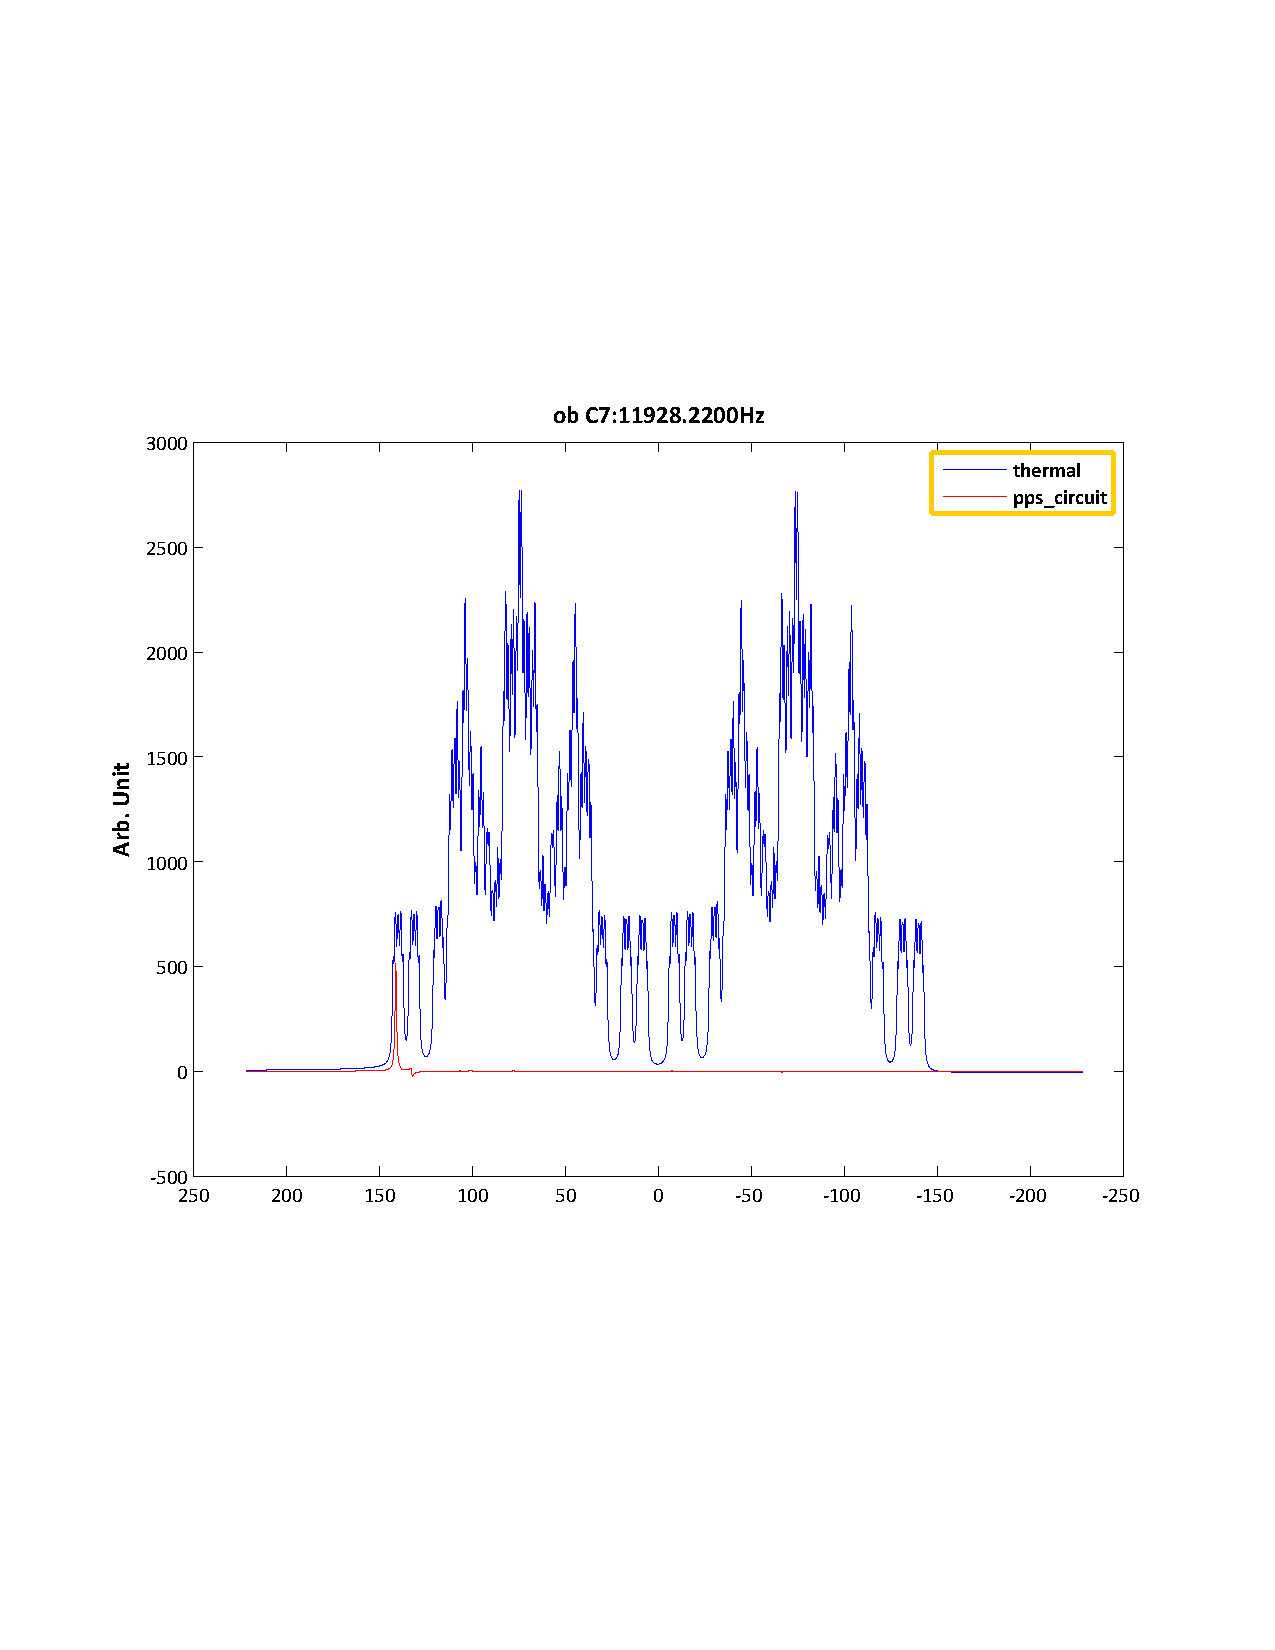
\includegraphics[width=\columnwidth]{thermal_and_pps_circuit.pdf}
\end{center}
\setlength{\abovecaptionskip}{-1cm}
\caption{\footnotesize{Comparison of the thermal and PPS produced by the circuit. }}\label{spectra}
\end{figure}

\clearpage
{\color{blue}{\textbf{Mar 11, 2015:}}}

\textbf{Use the GRAPE unitaries to simulate the 12-qubit PPS circuit again. The imperfection of the GRAPE pulses will contribute to some minor error in spectra.}

The unitaries for all rotations have been saved in Ordi2. So I only combined them with the free evolutions. \textbf{Note the time step is 10us, which means the free evolutions are integer times of 10us with the unwanted chemical shift refocusing (important!!!).}

Evolution times for every part.

Encoding1:
\begin{table}[hbtp]
\begin{tabular} {c||c|c|c|c|c|c}
  \hline
   Name & Total & $1/4\text{J}_{27}$ & $1/4\text{J}_{67}-1/4\text{J}_{27}$ & $1/4\text{J}_{47}-1/4\text{J}_{67}$ & $1/4\text{J}_{57}-1/4\text{J}_{47}$ & $1/4\text{J}_{57}$\\
  \hline
  Encoding1 & 32.98ms & 6670us & 560us & 1380us & 2880us & 11490us\\
  \hline
\end{tabular}
\end{table}

Encoding2:
\begin{table}[hbtp]
\begin{tabular} {c||c|c|c|c}
  \hline
   Name & Total & $1/4\text{J}_{12}$ & $1/4\text{J}_{23}-1/4\text{J}_{12}$ & $1/4\text{J}_{23}$\\
  \hline
  Encoding2 & 21.28ms & 4340us & 3300us & 7640us\\
  \hline
\end{tabular}
\end{table}

Encoding3:
\begin{table}[hbtp]
\begin{tabular} {c||c|c|c}
  \hline
   Name & Total & $1/4\text{J}_{\text{CH}}$ & $1/4\text{J}_{\text{CH}}$\\
  \hline
  Encoding3 & 7.36ms & 1680us & 1680us\\
  \hline
\end{tabular}
\end{table}

Decoding1:
\begin{table}[!h]
\begin{tabular} {c||c|c|c}
  \hline
   Name & Total & $1/4\text{J}_{\text{CH}}$ & $1/4\text{J}_{\text{CH}}$\\
  \hline
  Decoding1 & 6.36ms & 1680us & 1680us\\
  \hline
\end{tabular}
\end{table}

Decoding2:
\begin{table}[!h]
\begin{tabular} {c||c|c|c|c}
  \hline
   Name & Total & $1/4\text{J}_{12}$ & $1/4\text{J}_{23}-1/4\text{J}_{12}$ & $1/4\text{J}_{23}$\\
  \hline
 Decoding2 & 20.28ms & 4340us & 3300us & 7640us\\
  \hline
\end{tabular}
\end{table}

Decoding3:
\begin{table}[!h]
\begin{tabular} {c||c|c|c|c|c}
  \hline
   Name & Total & $1/4\text{J}_{27}$ & $1/4\text{J}_{27}$ & $1/4\text{J}_{57}$ & $1/4\text{J}_{57}$\\
  \hline
 Decoding3 & 42.32ms & 6670us & 6670us & 11490us & 11490us\\
  \hline
\end{tabular}
\end{table}

\textbf{Updated on April 6: Please ignore the following sentences as Annie found a mistake in check\_grape.m. The unitary of the GRAPE pulse should be U(4us)*Ugrape*U(4us), but I wrote Ugrape*U(8us) by mistake! This will introduce a serious phase error and trigger the following problem. I have fixed it.}
\emph{It is surprising that after applying phase cycling, the state will introduce a phase. The ideal state after phase cycling will have two elements 0.7071 at the top off-diagonal positions, but these two numbers change to 0.5018-0.4057i and  0.5018+0.4057i after GRAPE phase cycling pulse. The absolute value is 0.6453, which is reasonable. Moreover, the state in the decoding part will also involve an unexpected phase in every step. I guess the reason is the imperfections of the GRAPE pulses (some of them are pretty low like 80\% fidelity), and the 90 or 180 pulse cannot rotate or refocus the state to the desired axis completely. Anyway, in the following table, I will write both fidelities, with and without this phase correction.}

All fidelities $\text{tr}(\rho_\text{{ideal}}\rho_\text{real})$ calculated by the circuit itself and by the GRAPE pulses.
\begin{table}[!h]
\begin{tabular} {c||c|c|c}
  \hline
   Part & Length & Circuit Fidelity & GRAPE Fidelity\\
  \hline
 Encoding1 & 32.98ms & 1.0000 & 0.9831\\
 Encoding2 & 21.28ms & 1.0000 & 0.9717\\
 Encoding3 & 7.36ms & 0.9500 & 0.9124\\
 Phase Cycling & 1ms & 0.9511 & 0.9126\\
 Decoding1 & 6.36ms & 0.8717 & 0.8693\\
 Decoding2 & 20.28ms & 0.8570 & 0.8430\\
 Decoding3 & 43.32ms & 0.8570 & 0.8234\\
  \hline
\end{tabular}
\end{table}

\newpage
\begin{figure}[htb]
\begin{center}
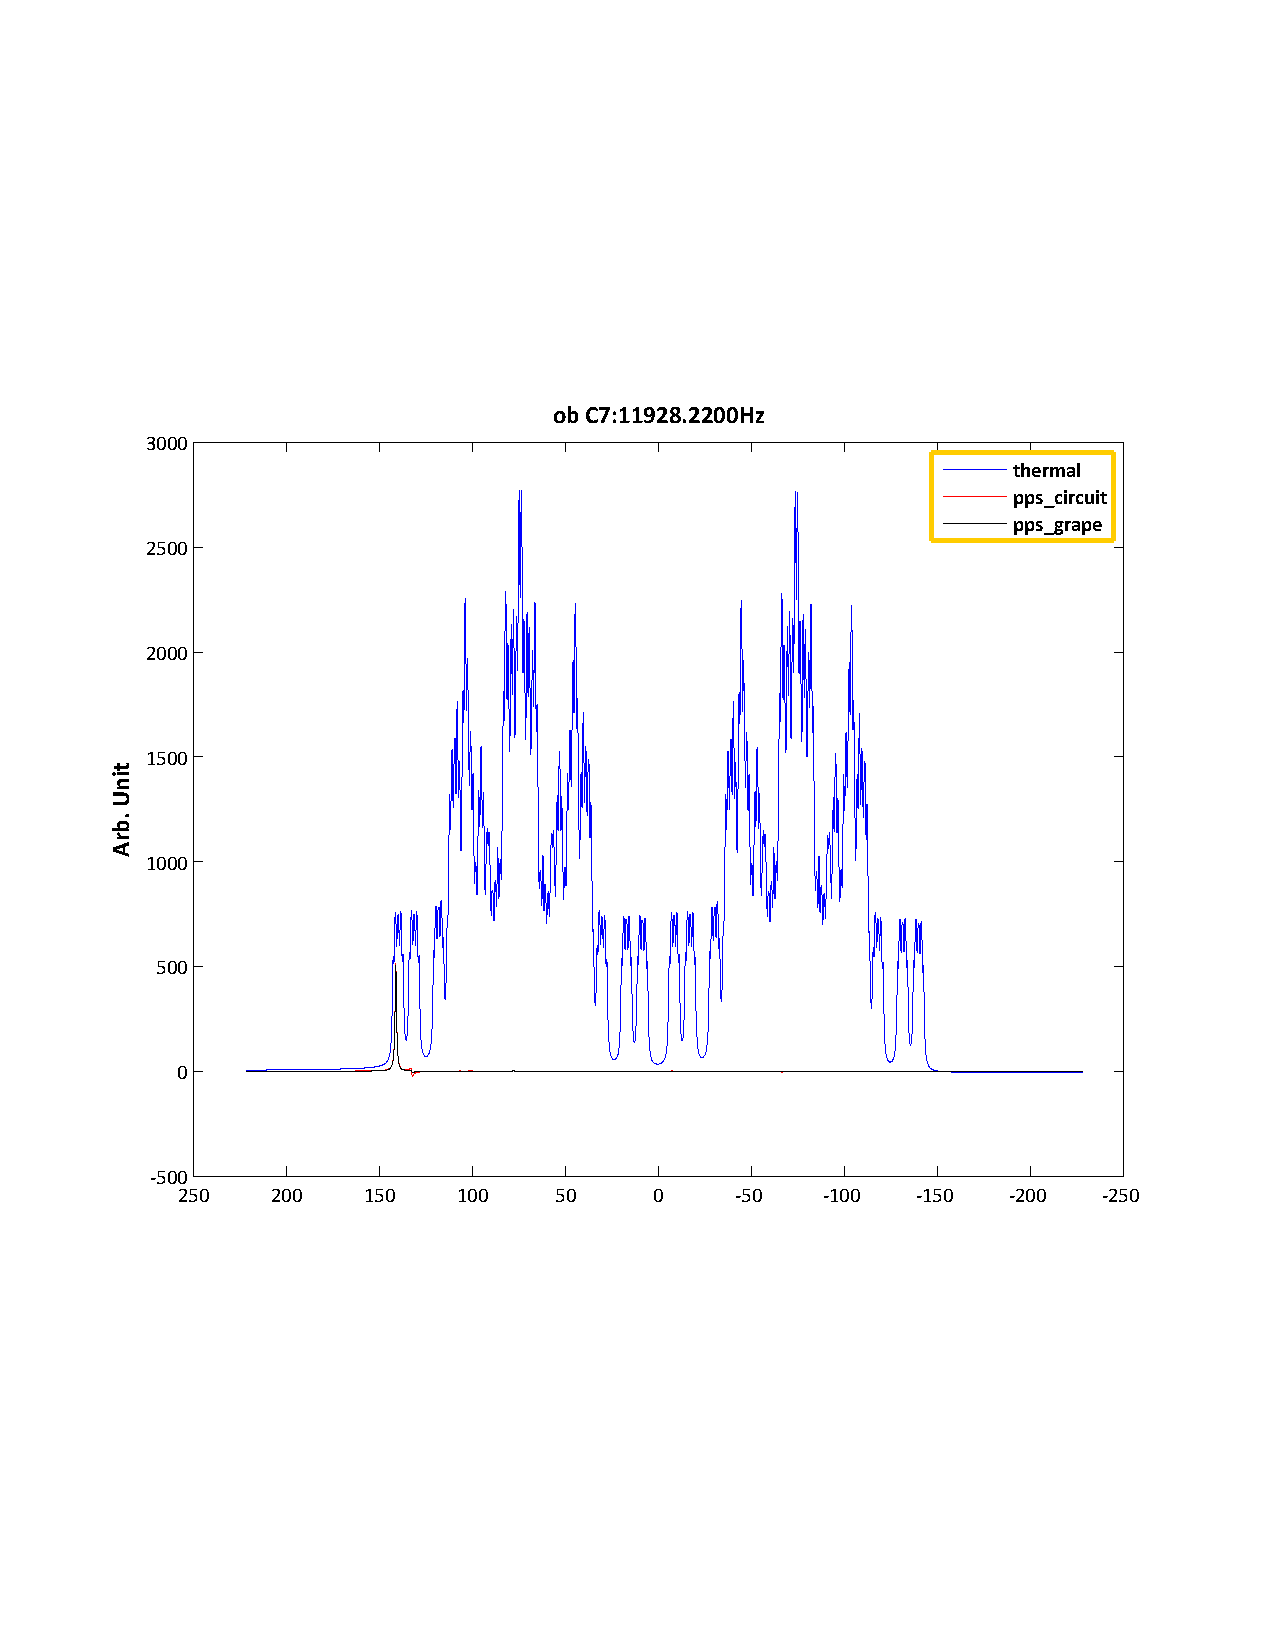
\includegraphics[width=\columnwidth]{thermal_and_pps_circuit_grape.pdf}
\end{center}
\setlength{\abovecaptionskip}{-1cm}
\caption{\footnotesize{Comparison of the thermal and PPS produced by the circuit and GRAPE. }}\label{compare_spectra}
\end{figure}

\clearpage
\section{June 09, 2015: Write a universal program for spectrum simulation}

\textbf{Fast spectrum generating code spec\_plot.m in \dir subfunction}

The previous way to simulate the NMR spectrum by giving the density matrix, Hamiltonian, T2* is via Fourier transform. The code is written by Colm Ryan and it is powerful. However, for 12 qubits it takes more than 40 minutes to get a spectrum. So I write another program to simulate the spectrum. It is universal, and only takes less than 1 minute for a 12-qubit simulation.

The function is 'spec\_plot.m' saved in the '\dir subfunction' folder. There are four input parameters: Hamiltonian, density matrix, observed spins and T2*. By giving the Hamiltonian, we can know the frequencies of all possible peaks. For example, in the 12-qubit sample we would like to observe C7. There should be $2^{11}$ peaks as 11 spins have interactions with C7. The central frequency is $\omega(7)$, which is the chemical shift of C7. So the frequency of all peaks would be
\be
\omega(7)+\sum_{i=1,i\neq 7}^{12} \pm J_{i7}/2.
\ee
By the signs of J, we can also know the state of the other qubits. I define +J/2 is $\ket{0}$ and -J/2 is $\ket{1}$ to make the $\ket{00..0}$ appear at  the leftmost side in Bruker (highest frequency). After confirming the state of the other qubits, we can convert this state to decimal number, and then know the locations of it in the density matrix, because the density matrix can be understood through states (row 1 is $\ket{00..0}$, row 2 is $\ket{00..1}$ etc.). The element in that position gives the real part and imaginary part of the related peak. Then a Lorentzian shape is plotted with this element as the amplitude and phase, and T2* as the half-height width. Sum over all the $2^{11}$ peaks will give the spectrum of C7. And if you want to save the figure and data points, just input a name after running the code. If you input 0, no data will be saved but the spectrum will be shown in a separate window.

\textbf{C2 fitting code fitting\_C2.m in \dir Twqubit\_Circuit\_PPS\dir simulation}

When I compared the thermal spectrum of C2 and experimental thermal, they do not match at the small J-couplings. This program is written to fit the small J-couplings of C2 by brutal force. I only need to fit the frequency 8900 to 8920 region as all small couplings are involved in it. There are 7 of them: C2C4, C2C5, C2C6, C2H1, C2H2, C2H3, and C2H5. Moreover, C2C4, C2C5, and C2C6 are fixed by the H-decoupled C spectrum. The second assumption is C2H2 and C2H3 have the same couplings to save time. The constraint is the width of this regions equals to the sum over all couplings, that is, only two variables then. C2H2 and C2H1.

The experimental spectrum is saved in 'thermal\_exp\_C\_200.mat' and the scaled factor is defined as the integral (sum) of the region [8900 8920]. There are 13 peaks in total and each peak corresponds to an intensity. In the fitting, we consider the 13 peak frequencies as the target function f, defined as the sum over square error of each peak. If this f is small then 1Hz which means the peak locations are pretty close, go to check the intensities of every peak. The definition of this value g is the same as f. When g is small, it means the peak intensities have the best fit as well as the locations are close too. The T2*=310ms gives the best match. Refer to the original code for details and the output spectrum is shown below (plotted by 'compared\_C2.m').

\begin{figure}
\begin{minipage}[hbtp]{0.5\linewidth}
\centering
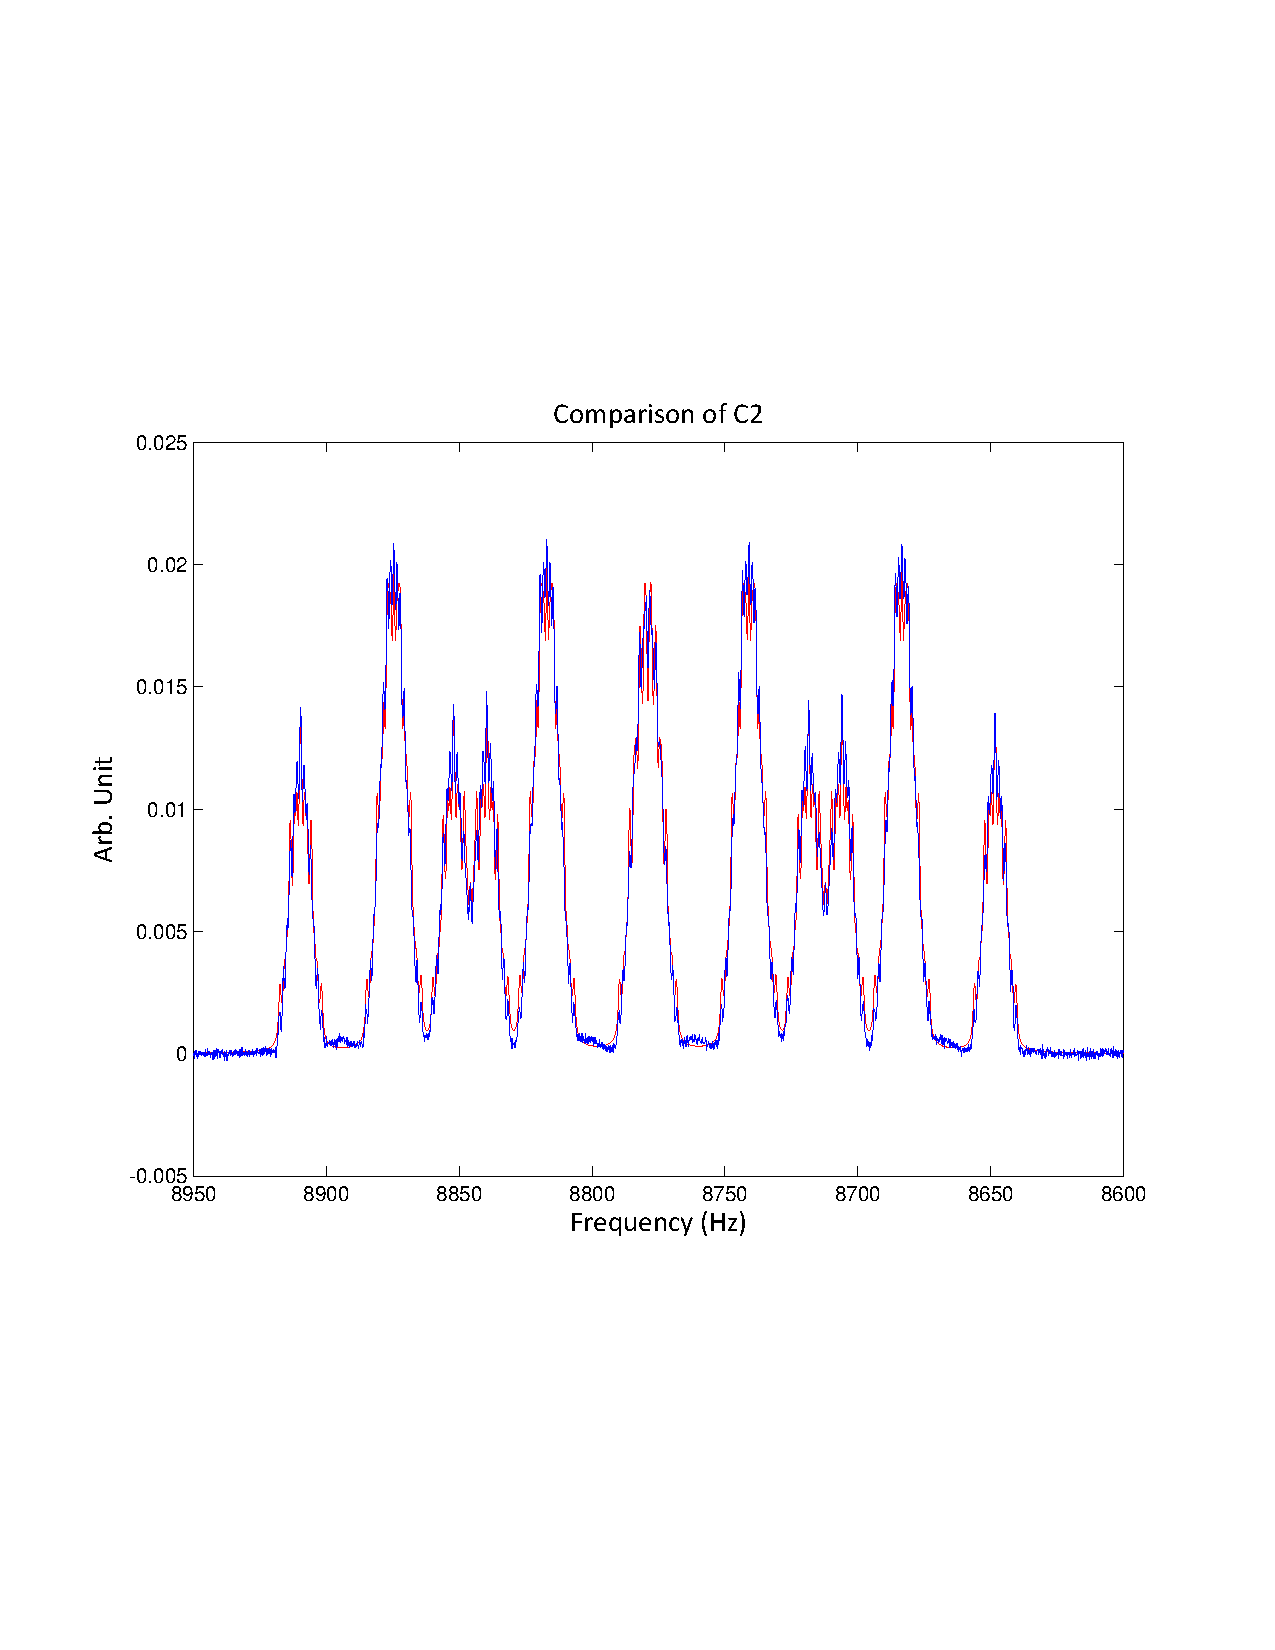
\includegraphics[width=0.8\columnwidth]{comparison_C2.pdf}
\caption{Comparison of simulated and experimental C2 thermal.}
\label{fig:side:a}
\end{minipage}%
\begin{minipage}[hbtp]{0.5\linewidth}
\centering
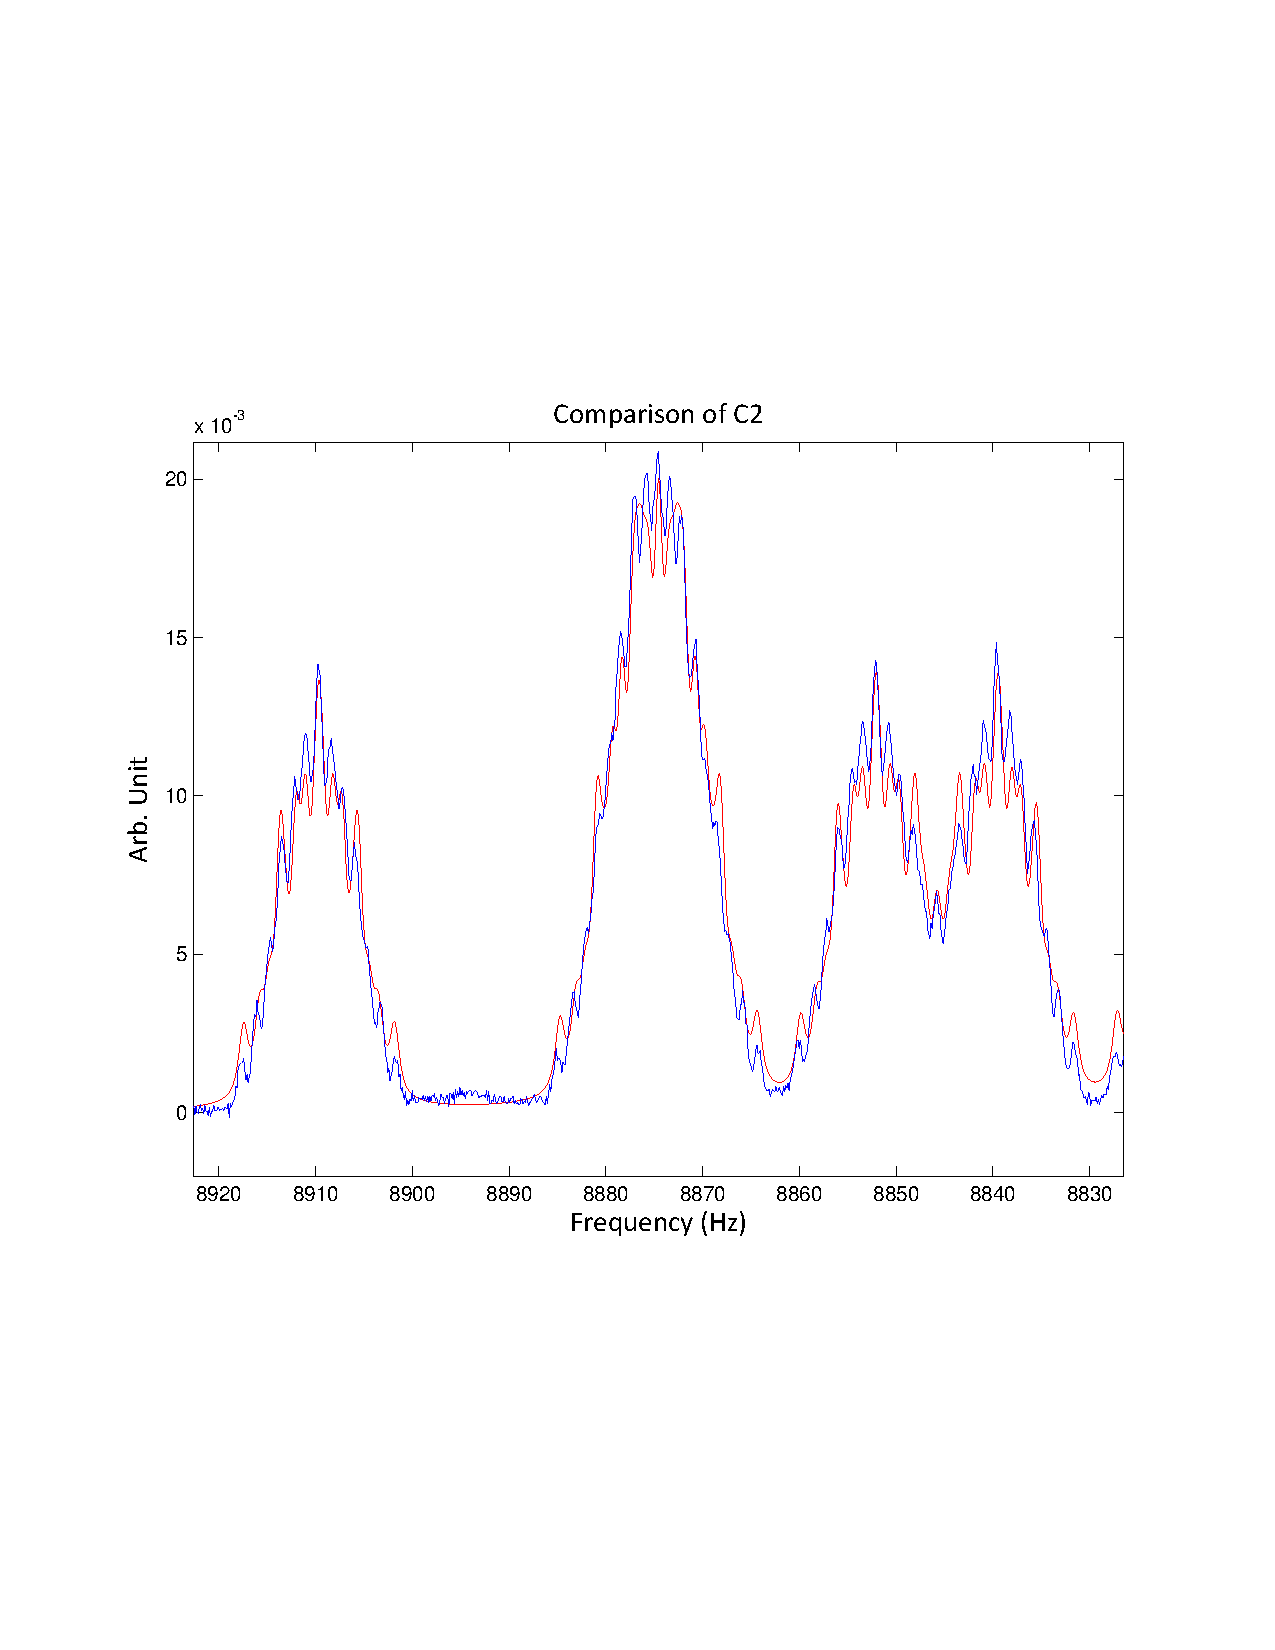
\includegraphics[width=0.8\columnwidth]{comparison_C2_zoomin.pdf}
\caption{Detailed comparison.}
\label{fig:side:b}
\end{minipage}
\end{figure}

Besides, C7 is also compared with T2*=420ms. The figure plotted by 'compared\_C7.m' is shown below.

\begin{figure}
\begin{minipage}[hbtp]{0.5\linewidth}
\centering
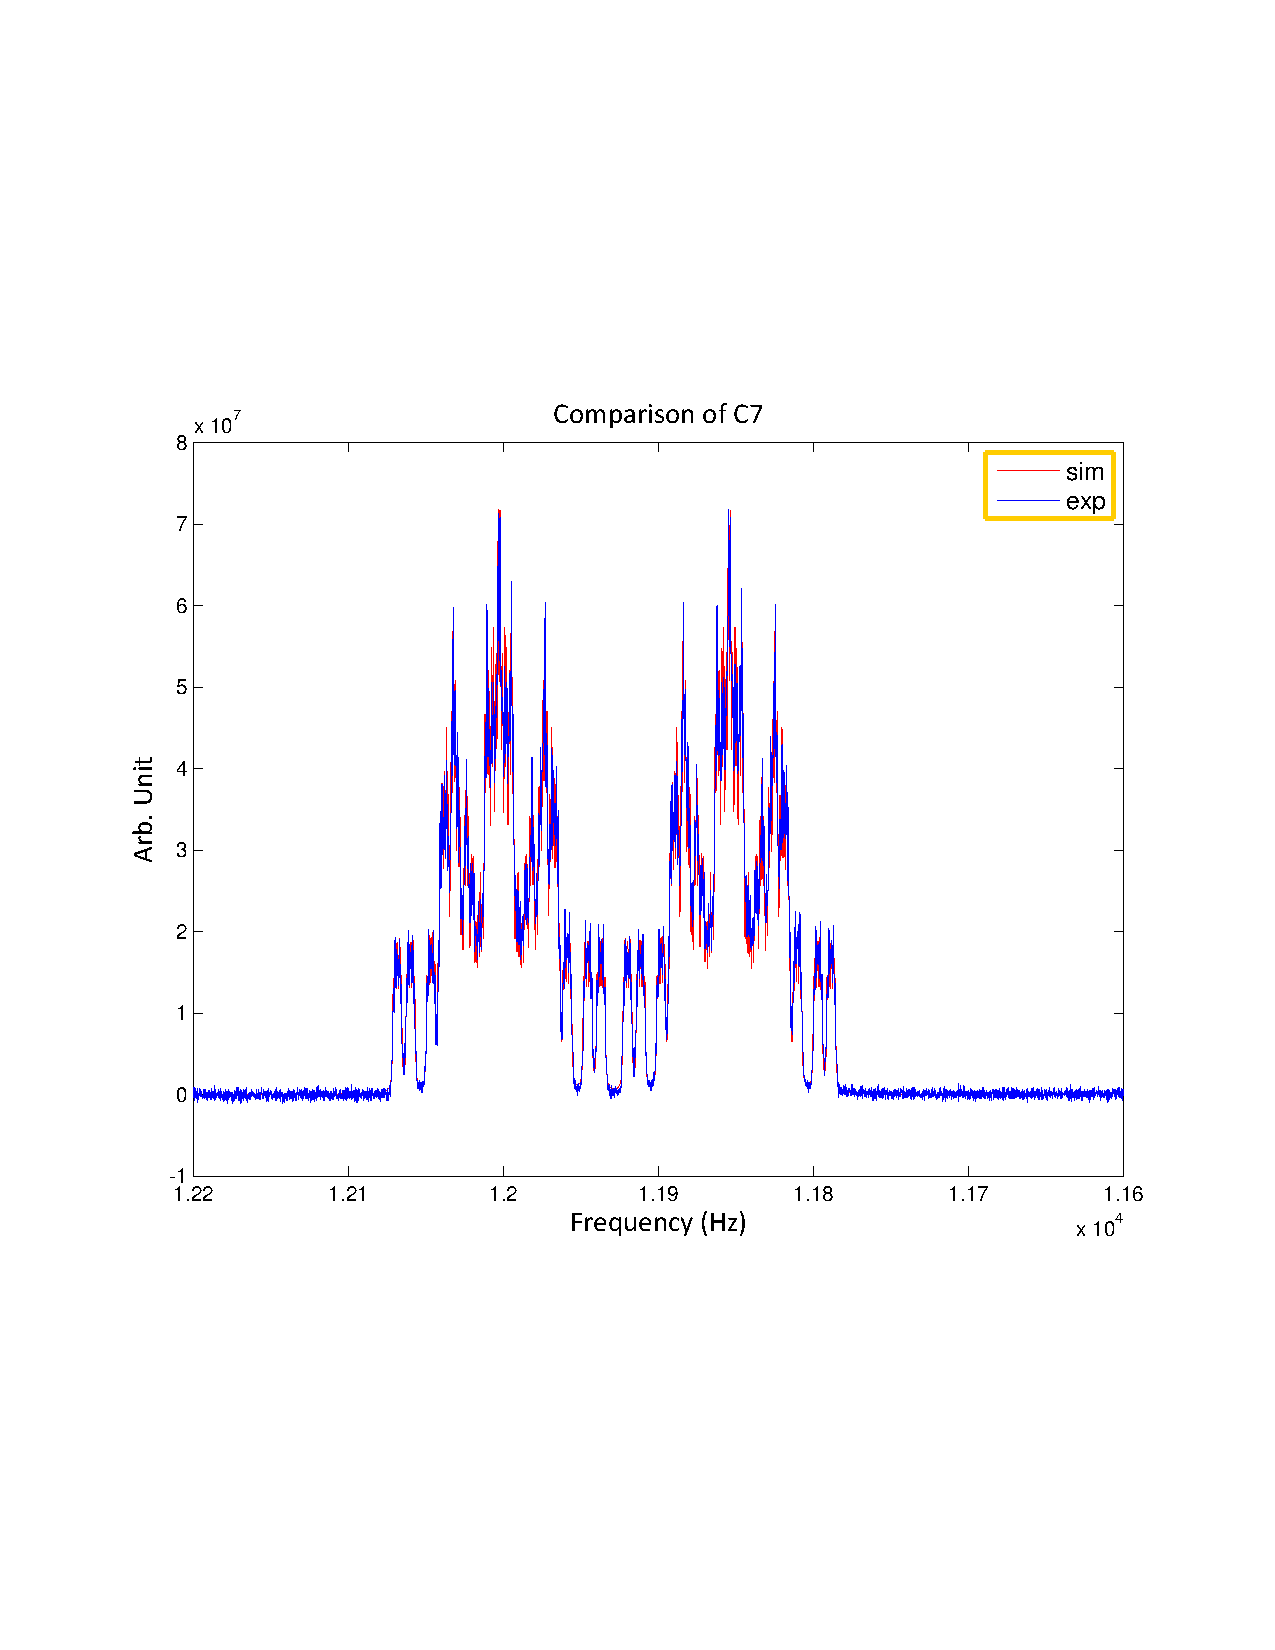
\includegraphics[width=0.8\columnwidth]{comparison_C7.pdf}
\caption{Comparison of simulated and experimental C7 thermal.}
\label{fig:side:a}
\end{minipage}%
\begin{minipage}[hbtp]{0.5\linewidth}
\centering
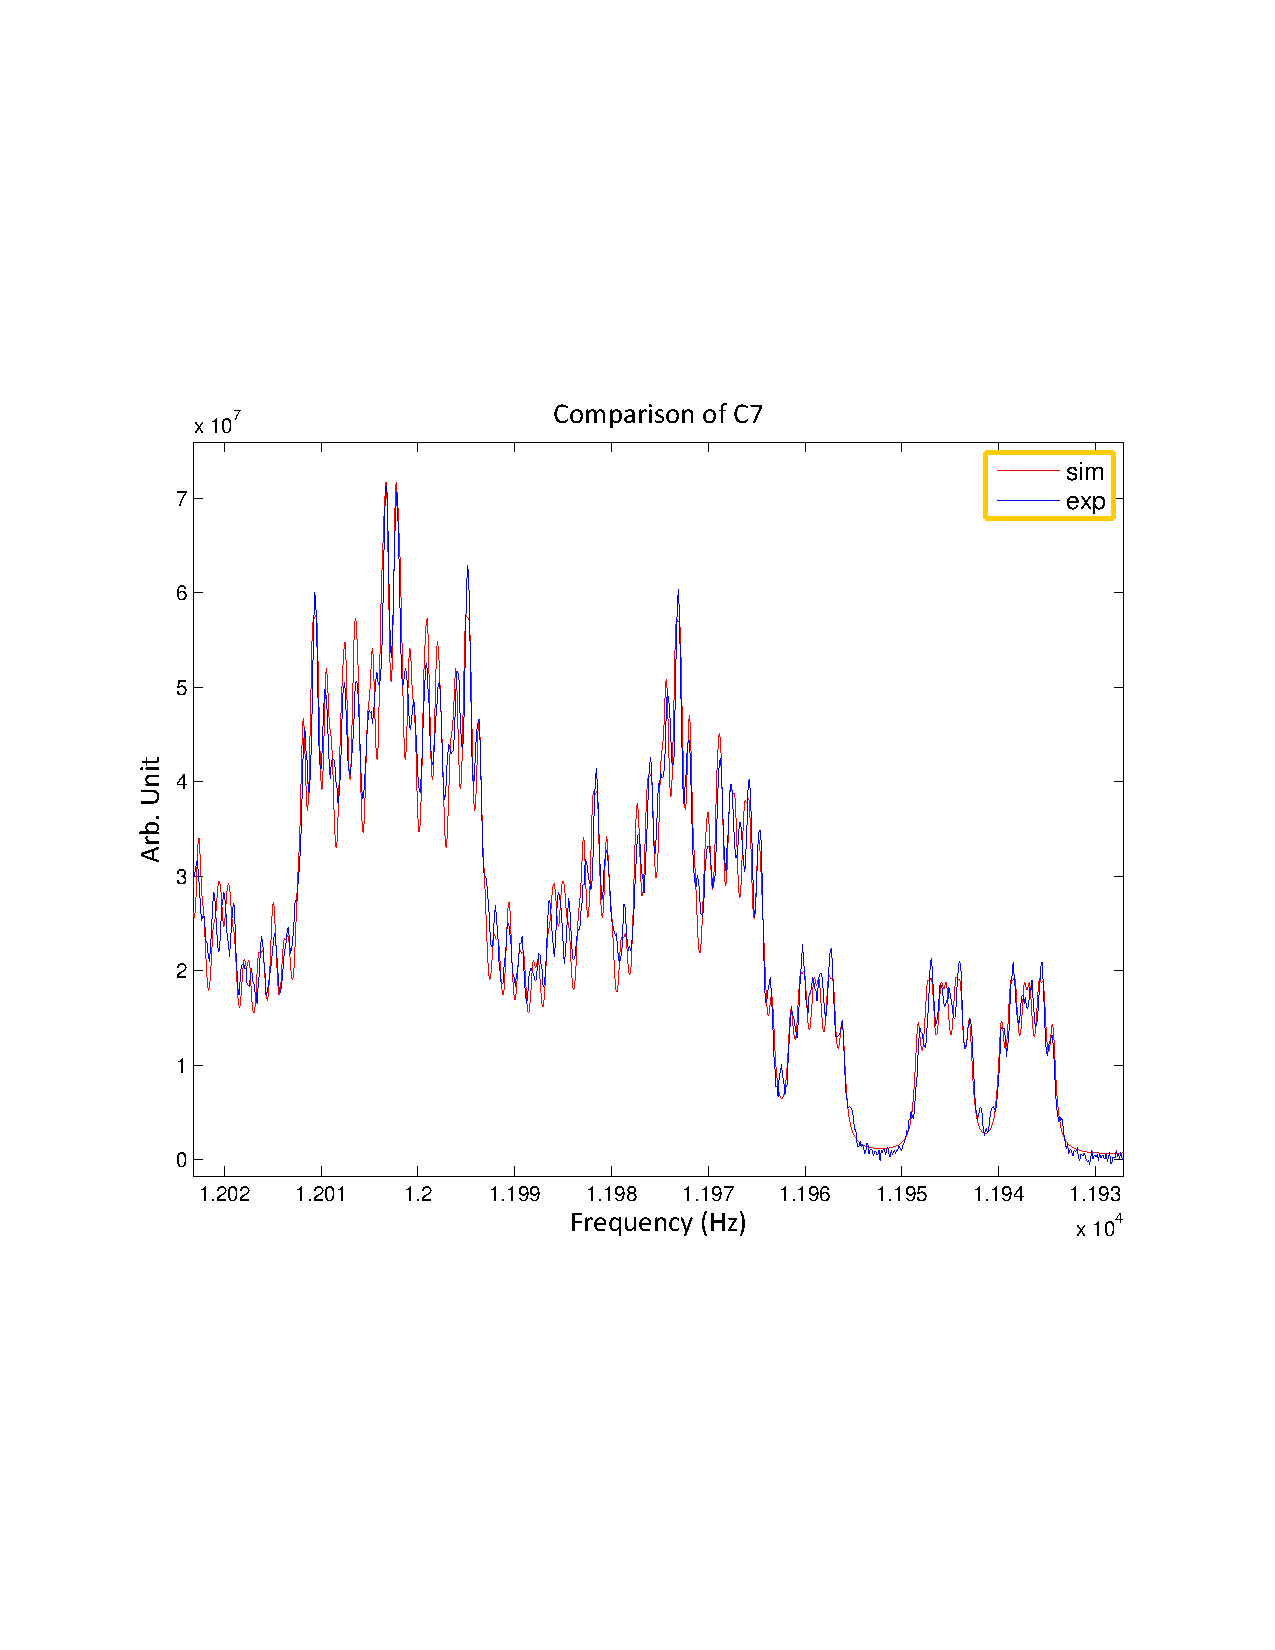
\includegraphics[width=0.8\columnwidth]{comparison_C7_zoomin.pdf}
\caption{Detailed comparison.}
\label{fig:side:b}
\end{minipage}
\end{figure}

Now it is ready to go to check every experimental spectrum of C2 and C7. Indeed, we will just observe these two.

\clearpage
\section{Apr 16, 2015: 12-qubit Calibration in Experiment}

The calibration is used for getting the dB of $\pi/2$ and $2\pi$ pulses for a fixed length. The au program is written by Annie, including 3 files 'calib.m', 'calibrate.m' and 'getspec.m'. First upload all the three files to Ordi2. Note 'calib.m' is for redirection and it should be in the root folder when opening Matlab in Ordi2. The path is thus '\dir d29lu\dir fixpulse\dir' because Matlab will go to this folder to show the last result of pulse fixing.

The calibration folder is 'twqubit\_calib'. Then select the experiment you want to calibrate, and run 'edau twqubit\_calib'. \textbf{You have to edit Line 6 'host\_resultpath', Line 24 'TIMES' which means number of loops, the following 'p1', 'd1' and 'pl3', and the starting power.  Then in 'calibrate.m', change the targetfolder, ob\_min, ob\_max and figure\_name. }

The experiments for calibrating C is titled 'twqubit\_calib\_C', and for calibrating H is 'twqubit\_calib\_H'. For H, I calibrated through the C channel as in experiment we only observe the C channel. The way is to transfer the H signal to C via XZ terms, so I can only calibrate the $\pi/2$ and $3\pi/2$ pulses. The results are summarized in the following table (\textbf{forget the column of June 25 as the setting is different and has been changed back})
\begin{table}[hbtp]
\begin{tabular} {c||c|c|c|c|c|c}
  \hline
  Rotation & Length & Frequency & Exp. No & dB (Apr 16) & dB (Apr 17) & dB (June 25)\\
  \hline
  % after \\: \hline or \cline{col1-col2} \cline{col3-col4} ...
  C360 & 40us & 25000Hz & 11-23 (-3.5dB to -5.9dB) & -4.51dB & -4.38dB & -1.18dB\\
  C360 & 80us & 12500Hz & 51-63 (3.0dB to 0.6dB) & 1.82dB & 1.74dB & ---\\
  C90 & 20us & 12500Hz & 101-113 (3.0dB to 0.6dB) & --- & 1.00dB\\
  H270 (by C) & 30us & 25000Hz & XXXX & --- & 6.20dB & 6.20dB\\
  H360 (by H) & 40us & 25000Hz & XXXX & --- & 5.40dB\\
  \hline
\end{tabular}
\end{table}

Actually only C360 and H270 are usable. The two powers are -4.38dB and 6.2dB for 25KHz.

\clearpage
\section{Apr 18, 2015 to Aug 18, 2015: All pulses test in experiment}

{\color{blue}{\textbf{Apr 18, 2015:}}}

\textbf{Tested all single-qubit pulses by a set of experiments for each. It is notable that when observing H channel as we have to set H channel as f1, the power calibration for H should be different from the setting that C is f1.}

The experimental folder is 'twqubit\_pps'. Exp 1 and 2 are thermal spectra.

For every pulse I have 4 observations. For C channel, for H channel, pulse-gradient-pulse for C channel, and pulse-gradient-pulse for H channel. Refer to the Appendix to see what the pulses are.

Polarization Crush \\
11-14: all90butC7

Phase Cycling \\
21-24: all90

Encoding \\
101-104: C57180 \\
105-108: C23180 \\
109-112: C234790 \\
113-116: C156180 \\
117-120: C234790withPC \\

Decoding \\
201-204: C2347andH180 \\
205-208: C134690andH90 \\
209-212: C23456180 \\
213-216: C1234690withPC \\
217-220: C27180 \\
221-224: C2Y5X90 \\

Single $\pi/2$ rotations \\
301-314: C1 to C7 90 rotation (two experiments for one pulse)

Single $\pi/2$ rotations \\
315-342: C1 to C7 180 rotation (four experiments for one pulse)

{\color{blue}{\textbf{Apr 23, 2015:}}}

\textbf{First try on the entire 12-qubit PPS circuit. One problem is found that the default 4us delay when calculating GRAPE pulses should be waived. So this part is not useful any more.}

Exp 1000: zg for the thermal without H decoupled \\
Exp 1001: observe C7 after crushing all the other 6 carbons and a gradient \\
Exp 1002: the same as 1001 but decoupled H before observing C7 \\
Exp 1003: Encoding 1. observe C7 and decouple H. Almost the same as the 7-qubit experiment. \\
Exp 1004: Encoding 2. observe C7 and decouple H. Almost the same as the 7-qubit experiment. \\
Exp 1005: PPS, gradient and observe C7 but no signal... \\
Exp 1006: PPS, without gradient and observe C7, no signal either... \\

\hypertarget{found:pulse_no_buffer}{There is a problem when I calculated the GRAPE.} There is a default 4us pre-delay and post-delay on the target unitary, as in experiment when applying the GRAPE pulse these two delays are required (not the minimal value but since GRAPE has considered that it has no effect). However, we do not have enough slots (only SP0 to SP31) for GRAPE pulses so we have to combine them to a big shape. The problem is the time step in the big shape is chosen as 10us, which cannot absorb the 4us delay. If we get rid of the 4us delays during the big shape, the experimental result is totally different.

I tried to use 2us time step size in the big shape instead of 10us, so I can write the 4us delay. Then for every 5 steps (2us*5=10us) the amplitude and the phase should be the same. In principal it is fine, but when I am fixing the pulse on the H channel, the random noise is so serious that we have to use a low-pass filter to remove the noise. As in the big shape the shape is not smooth any more, some wanted points will be removed by the filter too. I guess no way to solve this except the pulse is smooth.

So maybe need recalculation with 0us pre-delay and post-delay. Please refer to \hyperlink{reason:pulse_no_buffer}{here} to know the details of the new 0us delay pulses.

{\color{blue}{\textbf{May 13, 2015:}}}

\textbf{New test with the No Buffer Pulses. Found a problem in pulse fixing and explained here. This part is no longer useful.}

Tested in experiment with the new no-buffer GRAPE pulses. I can still get the 7 coherence by decoupling H channel. To my surprise, if I fixed all the pulses, the performance with the fixed ones is even worse. I guess the reason is when pulse fixing, the baseline is a little bit below 0 for the free evolution. It does not make sense to fix them but the fixing program is indeed trying to fix it. The solution might be fixing each pulse one by one, and then combine all of them with the 0 points for free evolution. It will be done soon.

Exp 1103: Ob Z24567 with H decoupling and non-fixed No Buffer pulses. Look good. \\
Exp 1104: Ob Z1234567 with H decoupling and non-fixed No Buffer pulses. Look good. \\
Exp 2103: Ob Z24567 with H decoupling and fixed No Buffer pulses. Worse than 1103, which is surprising. \\
Exp 2104: Ob Z1234567 with H decoupling and fixed No Buffer pulses. Worse than 1104, which is surprising. \\

For PPS, there is still no signal. See Exp 1999 and 2000.
Exp 1999: PPS by non-fixed No Buffer pulses. No signal. \\
Exp 2000: PPS by fixed No Buffer pulses. No signal. \\

I tried 'fp' with about 200 scans to get a signal after one phase cycling step, and 80 scans with 'efp' and 'LB=0.3Hz'. So I divided the PPS into 24 experiments, and 80 scans for each experiment. D1 = 60s, so the total time for trying a PPS now is 34 hours...

\textbf{Note: Explanations to Exp 2103 and 2104.} The No Buffer pulses after fixing are even worse because the fixing program has a problem. The pulses itself is a big shape, with tons of 0 points inside to realize free evolutions. However, the pickup coil will detect slight signals for those 0 points (slightly over or below 0). The fixing program tries to correct these points by modifying these 0 to non-zero, which is not reasonable. One way to solve this problem is by fixing all pulses individually and combine them at last. So I fixed all the 18 pulses either 1ms or 2ms, and then used programs called 'pulse\_combine\_encoding\_nobuffer\_fixed.m' and 'pulse\_combine\_decoding\_nobuffer\_fixed.m' in '\dir Twqubit\dir Pulses\_NoBuffer\dir' to combine all of them with 0 points.

Unfortunately the result is not good. It turns out that the signal is still very low with 80 scans. So maybe improve the number of scans can help a little bit.

{\color{blue}{\textbf{May 22, 2015:}}}

\textbf{Re-run PPS with Scan=200. No signal again but the 24 experimental settings (Exp 2001 to Exp 2024) will be used in the future.}

As there are three days that we will go to Ray's cottage, I set 200 scans for each phase cycling and the total length is thus 3d10hrs. I used a MAC program to automatically set all 24 experimental parameters. The Matlab program to generate this MAC file is 'Genmultizg.m' in '\dir Twqubit\dir'. Put the generated file to '\dir lists\dir mac\dir'. The 24 experiments are from Exp 2001 to Exp 2024.

Unfortunately there is no FID after the multizg. I tried some of the 24 experiments and they cannot do fp or efp. Need to figure out why. Another problem is during a long multizg, the sample will unlock at some time. Xinhua said the reason is gradient field. Because the gradient field is applied in z direction, it will affect the locking signal. But we cannot avoid the many gradient fields in between. Try experiment one by one? Anyway, do simulation now. That is, getting the simulated spectrum of each phase cycling, and then compare.

Re-run the 24 experiments again and now they have spectrum. Almost all 0. The sum is not a single peak. Meanwhile, the simulation is done. The folder is '\dir Twqubit\_Circuit\_PPS\dir'. First I ran 'rho\_phasecycling\_24steps.m' to get all MAT files of the 24 states, with each one corresponding to a phase cycling step. Then upload all the 24 MAT files to Ordi2 where the 'mkstate.m' function is. Run 'sim\_12pps\_step.m' in '\dir NMR\dir EXPERIMENTS\dir twqubit' to get all the simulated results and transfer them to my laptop. Plot all the 24 figures with the name such as '24\_step\_7.fig' for each one. Every spectrum out of the 24 figures is oscillating seriously which means if the T2* is not long enough (the case in experiment), we cannot resolve it.

{\color{blue}{\textbf{June 11, 2015:}}}

\textbf{Found the best parameters for 12 qubits.}

Before experiments, I want to find the best setting for 12 qubits.

\textbf{SWH = 30030Hz. DW = 16.65us. }\\
SWH is a fixed value. DW is related to the sampling rate, and reciprocal (inversely proportional) to SWH.

\textbf{TD = 65536 and SI = 262144(max).} \\
The real spectrum will have SI points. So if SI<TD, it will cut the first SI points from TD when doing FFT. Otherwise, it will add the number of SI-TD points to the tail when doing FFT. Because SWH is very big, we need many many points to keep a high resolution. That is why SI is so big. Meanwhile, if TD is much smaller, we will use a lot of zero points added to the tail of TD, which means the noise is canceled a lot. Small TD gives us a good SNR, but it loses the resolution of small couplings.
\textbf{(For H-decoupled experiments, TD = 281684 for a high resolution.)}

\textbf{AQ = 1.09s.}\\
AQ is fixed as AQ = DW*TD.

{\color{blue}{\textbf{Still Keep Updating:}}}

\textbf{Implement every encoding and decoding part and compare with simulation.}

The experiments are (Spectra are shown in Appendix II).

Exp 1398: Observe C7 by Gaussian with H decoupled. NS = 1. TD=281684. \\
Exp 1399: Observe C2 by Gaussian with H decoupled. NS = 1. TD=281684. \\
Exp 1401: Observe C7 by GRAPE as the reference. NS=10. See Fig. \ref{1401and1402}\\
Exp 1402: Observe C2 by GRAPE as the reference. NS=10. To my surprise the phase is different with 1401.\\
Exp 1403: Observe C7 after encoding1. NS=10. See Fig. \ref{1403and1404}\\
Exp 1404: Observe C2 after encoding1. NS=10.\\
Exp 1405: Observe C7 after encoding1 and decouple H. NS=1. See Fig. \ref{1405and1406}\\
Exp 1406: Observe C2 after encoding1 and decouple H. NS=1.\\
Exp 1407: Observe C7 after encoding2. NS=10. See Fig. \ref{1407and1408}\\
Exp 1408: Observe C2 after encoding2. NS=10.\\
Exp 1409: Observe C7 after encoding2 and decouple H. NS=1. See Fig. \ref{1409and1410}\\
Exp 1410: Observe C2 after encoding2 and decouple H. NS=1.\\

For encoding3 which generates ZZZZZZZZZZZZ, we tested that it cannot be observed. The H channel cannot be decoupled as the state of H is not I. So we directly applied encoding 3 to thermal state, and C-H couplings will evolve.

Exp 1411: Observe C7 after encoding3, applied on thermal. NS=1. See Fig. \ref{1411and1412}\\
Exp 1412: Observe C2 after encoding3, applied on thermal. NS=1.\\
Exp 1413: Observe C3 after encoding3, applied on thermal. NS=1.\\
Exp 1414: Observe C4 after encoding3, applied on thermal. NS=1.\\

Prepare the 7-qubit PPS and replace some of the pulses with the 12-qubit GRAPE. This can check the performance of these 12-qubit GRAPE pulses. All the sequences have a C-H SWAP in the very beginning to improve the C signal.

Exp 1887: Observe C7 on thermal. NS=7. See Fig. \ref{1887and1888}\\
Exp 1888: Observe C7 after C-H SWAP applied on thermal. NS=7.\\
Exp 1889: Observe C7 of the 7-qubit PPS. NS=7. See Fig. \ref{1888and1889}\\
Exp 1891: Observe C7 of the 7-qubit PPS, with the Encoding replaced by 12-qubit pulses. NS=7.\\
Exp 1893: Observe C7 of the 7-qubit PPS, with the Encoding and Phase Cycling replaced by 12-qubit pulses. NS=7. See Fig. \ref{1889and1891and1893}\\

\clearpage
\section{Appendix I: Useful Matlab Codes}
\hypertarget{code:check_grape}{The code to check all the 12-qubit GRAPE fidelities:}
\begin{lstlisting}
load Para.mat
load twpauliX_full.mat
load twpauliY_full.mat

%% Check all 90 rotations
for spin_number = 1:7
Name1 = ['twqubit_C', num2str(spin_number), '90_C_25000.txt'];
Name2 = ['twqubit_C', num2str(spin_number), '90_H_25000.txt'];
Amplitude = 25000;
Time = 1e-3;
Length = 100;
dt = Time/Length;
FirstLine = 19; % the first line which contains power and phase

Output1 = 'test1';
Output2 = 'test2';

[power1,phase1]=dataout(Name1,Output1,FirstLine,Length);
[power2,phase2]=dataout(Name2,Output2,FirstLine,Length);
%% Check
X_C = 0; Y_C = 0;
for jj = 1:7
    X_C = X_C + KIx{jj};
    Y_C = Y_C + KIy{jj};
end

X_H = 0; Y_H = 0;
for jj = 8:12
    X_H = X_H + KIx{jj};
    Y_H = Y_H + KIy{jj};
end

U = eye(2^12);
U = U*expm(-i*H*4e-6);
for ii = 1:Length
    Hext = 2*pi*(Amplitude*power1(ii)/100)*(X_C*cos(phase1(ii)/360*2*pi)-Y_C*sin(phase1(ii)/360*2*pi))+2*pi*(Amplitude*power2(ii)/100)*(X_H*cos(phase2(ii)/360*2*pi)-Y_H*sin(phase2(ii)/360*2*pi));
    U = expm(-i*(Hext+H)*dt)*U;
end
U = U*expm(-i*H*4e-6);

Utar = expm(-i*KIx{spin_number}*pi/2);

Fidelity = abs(trace(U*Utar'))/2^12

savefile = ['twqubit_C', num2str(spin_number), '90_Ufid.mat'];
save (savefile, 'U', 'Fidelity');

end
\end{lstlisting}

\clearpage
\hypertarget{code:combine_encoding1}{The code to combine GRAPE pulses into a big shape file:}
\begin{lstlisting}
%% From Z7 to Z24567
step_27 = round(1/(4*Para(2,7))/dt);
step_67_27 = round((1/(4*Para(6,7))-1/(4*Para(2,7)))/dt);
step_47_67 = round((1/(4*Para(4,7))-1/(4*Para(6,7)))/dt);
step_57_47 = round((1/(4*Para(5,7))-1/(4*Para(4,7)))/dt);
step_57 = round((1/(4*Para(5,7)))/dt);

power_encoding1_C = [power_C790_C; zeros(step_27,1);power_C2180_C; zeros(step_67_27,1); power_C6180_C; zeros(step_47_67,1);power_C4180_C; zeros(step_57_47,1);...
                                  power_C5180_C; power_C7180_C; zeros(step_57,1);power_C790_C]*Calibration/Calibration_old;
phase_encoding1_C = [phase_C790_C; zeros(step_27,1);phase_C2180_C; zeros(step_67_27,1); phase_C6180_C; zeros(step_47_67,1);phase_C4180_C; zeros(step_57_47,1);...
                                  phase_C5180_C; phase_C7180_C; zeros(step_57,1);mod((phase_C790_C+90),360)];
power_encoding1_H = [power_H790_H; zeros(step_27,1);power_H2180_H; zeros(step_67_27,1); power_H6180_H; zeros(step_47_67,1);power_H4180_H; zeros(step_57_47,1);...
                                  power_H5180_H; power_H7180_H; zeros(step_57,1);power_H790_H]*Calibration/Calibration_old;
phase_encoding1_H = [phase_H790_H; zeros(step_27,1);phase_H2180_H; zeros(step_67_27,1); phase_H6180_H; zeros(step_47_67,1);phase_H4180_H; zeros(step_57_47,1);...
                                  phase_H5180_H; phase_H7180_H; zeros(step_57,1);mod((phase_H790_H+90),360)];

total_time_encoding1 = length(power_encoding1_C)*dt;

outputfile = 'twqubit_encoding1_C';
shpfile = fopen(outputfile,'w');
    fprintf(shpfile,'##TITLE= %s\n',outputfile);
    fprintf(shpfile,'##JCAMP-DX= 5.00 Bruker JCAMP library\n');
    fprintf(shpfile,'##DATA TYPE= Shape Data\n');
    fprintf(shpfile,'##ORIGIN= Dawei''s GRAPE Pulses \n');
    fprintf(shpfile,'##OWNER= Dawei\n');
    fprintf(shpfile,'##DATE= %s\n',date);
    time = clock;
    fprintf(shpfile,'##TIME= %d:%d\n',fix(time(4)),fix(time(5)));
    fprintf(shpfile,'##MINX= %7.6e\n',min(power_encoding1_C));
    fprintf(shpfile,'##MAXX= %7.6e\n',max(power_encoding1_C));
    fprintf(shpfile,'##MINY= %7.6e\n',min(phase_encoding1_C));
    fprintf(shpfile,'##MAXY= %7.6e\n',max(phase_encoding1_C));
    fprintf(shpfile,'##$SHAPE_EXMODE= None\n');
    fprintf(shpfile,'##$SHAPE_TOTROT= %7.6e\n',90);
    fprintf(shpfile,'##$SHAPE_BWFAC= %7.6e\n',1);
    fprintf(shpfile,'##$SHAPE_INTEGFAC= %7.6e\n',1);
    fprintf(shpfile,'##$SHAPE_MODE= 1\n');
    fprintf(shpfile, '##PULSE_WIDTH= %d\n',total_time_encoding1);
    fprintf(shpfile, '##Calibration_Power= %d\n',Calibration);
    fprintf(shpfile,'##NPOINTS= %d\n',length(power_encoding1_C));
    fprintf(shpfile,'##XYPOINTS= (XY..XY)\n');

for ii = 1:length(power_encoding1_C)
    fprintf(shpfile,'  %7.6e,  %7.6e\n',power_encoding1_C(ii),phase_encoding1_C(ii));
end

    fprintf(shpfile,'##END=\n');

outputfile = 'twqubit_encoding1_H';
shpfile = fopen(outputfile,'w');
    fprintf(shpfile,'##TITLE= %s\n',outputfile);
    fprintf(shpfile,'##JCAMP-DX= 5.00 Bruker JCAMP library\n');
    fprintf(shpfile,'##DATA TYPE= Shape Data\n');
    fprintf(shpfile,'##ORIGIN= Dawei''s GRAPE Pulses \n');
    fprintf(shpfile,'##OWNER= Dawei\n');
    fprintf(shpfile,'##DATE= %s\n',date);
    time = clock;
    fprintf(shpfile,'##TIME= %d:%d\n',fix(time(4)),fix(time(5)));
    fprintf(shpfile,'##MINX= %7.6e\n',min(power_encoding1_H));
    fprintf(shpfile,'##MAXX= %7.6e\n',max(power_encoding1_H));
    fprintf(shpfile,'##MINY= %7.6e\n',min(phase_encoding1_H));
    fprintf(shpfile,'##MAXY= %7.6e\n',max(phase_encoding1_H));
    fprintf(shpfile,'##$SHAPE_EXMODE= None\n');
    fprintf(shpfile,'##$SHAPE_TOTROT= %7.6e\n',90);
    fprintf(shpfile,'##$SHAPE_BWFAC= %7.6e\n',1);
    fprintf(shpfile,'##$SHAPE_INTEGFAC= %7.6e\n',1);
    fprintf(shpfile,'##$SHAPE_MODE= 1\n');
    fprintf(shpfile, '##PULSE_WIDTH= %d\n',total_time_encoding1);
    fprintf(shpfile, '##Calibration_Power= %d\n',Calibration);
    fprintf(shpfile,'##NPOINTS= %d\n',length(power_encoding1_H));
    fprintf(shpfile,'##XYPOINTS= (XY..XY)\n');

for ii = 1:length(power_encoding1_H)
    fprintf(shpfile,'  %7.6e,  %7.6e\n',power_encoding1_H(ii),phase_encoding1_H(ii));
end

    fprintf(shpfile,'##END=\n');
\end{lstlisting}

\clearpage
\section{Appendix II: Important Figures and Experimental Spectra}
Exp 1401: Observe C7 by GRAPE as the reference. NS=10.\\
Exp 1402: Observe C2 by GRAPE as the reference. NS=10. \\

\begin{figure}[htb]
\begin{center}
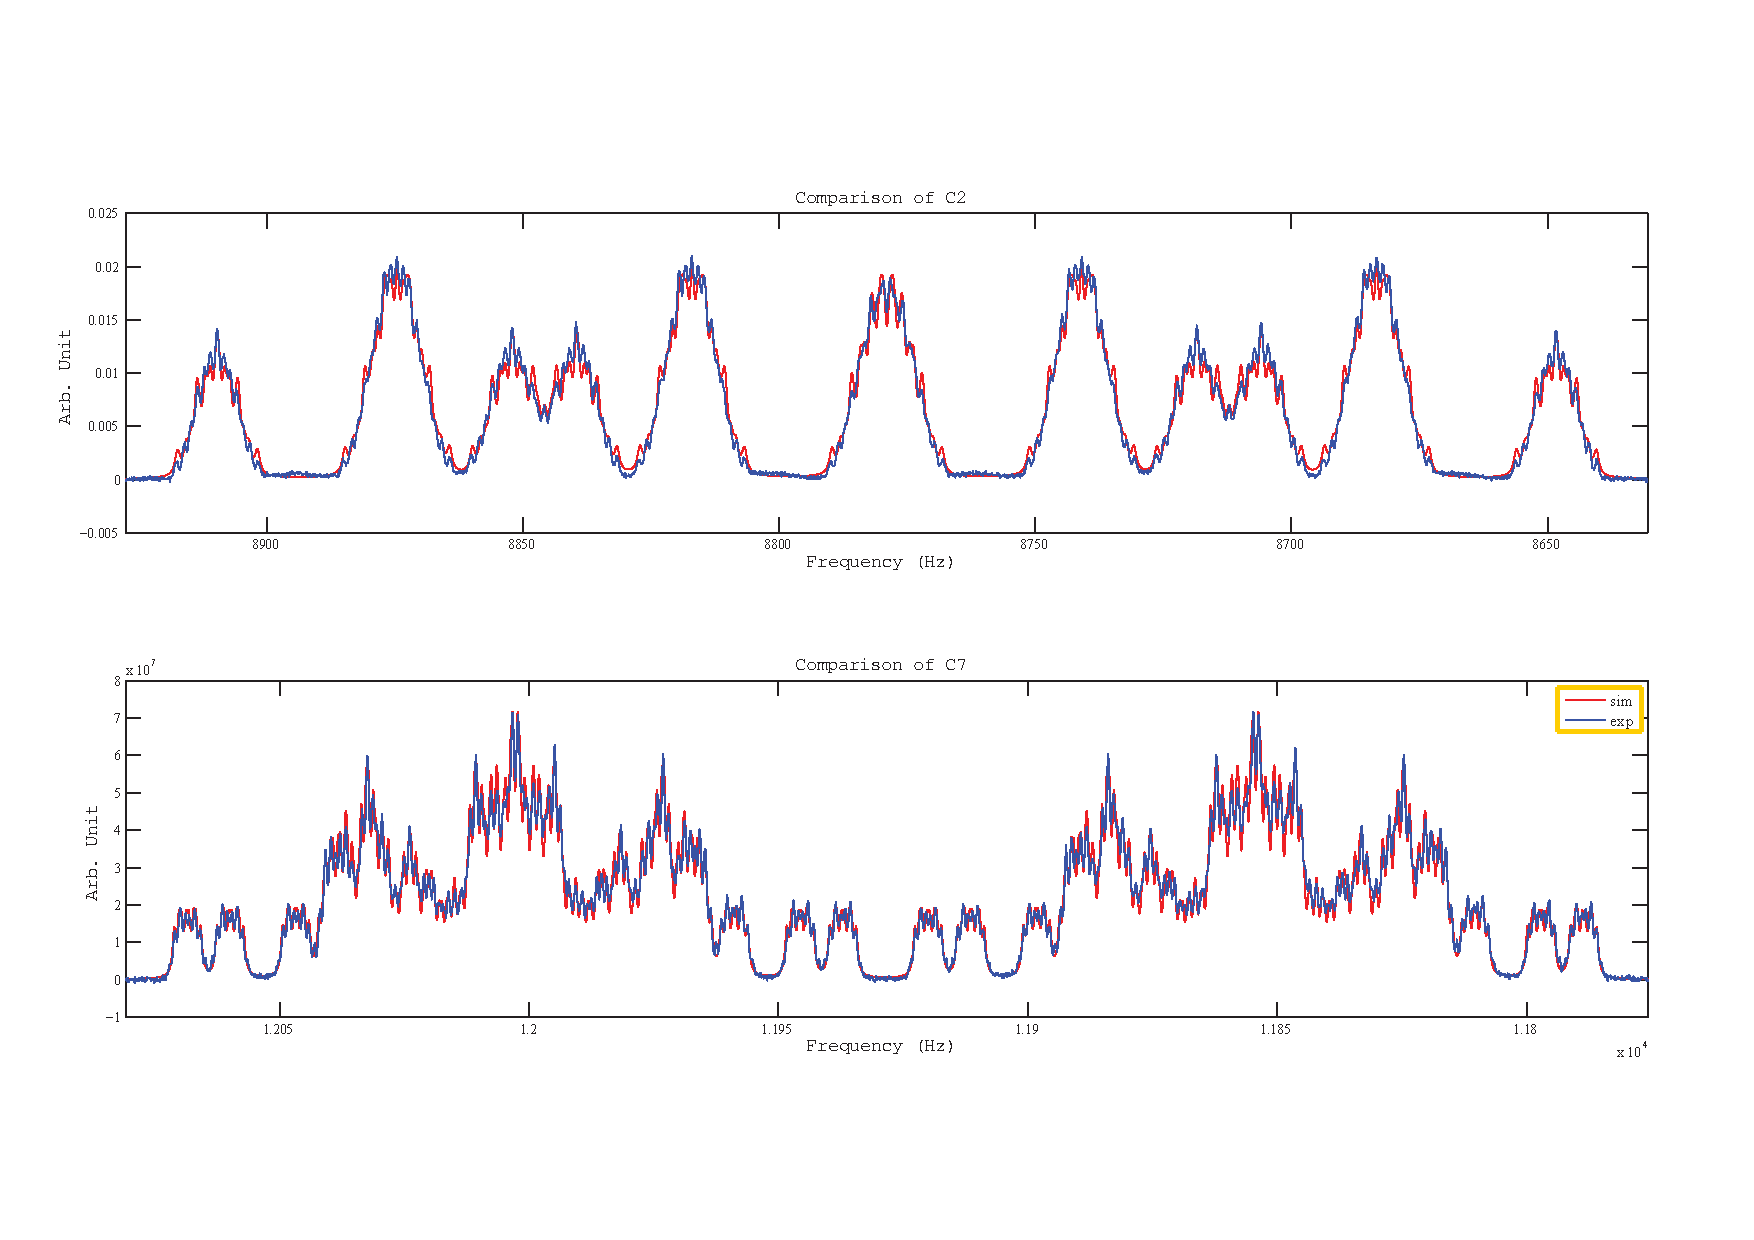
\includegraphics[width=\columnwidth]{Thermal_C2andC7.pdf}
\end{center}
\setlength{\abovecaptionskip}{-0.35cm}
\caption{\footnotesize{Comparison of the thermal for C2 and C7. Blue is experiment and Red is the simulation by the fitted Hamiltonian.}}\label{1401and1402}
\end{figure}

\clearpage
Exp 1403: Observe C7 after encoding1. NS=10.\\
Exp 1404: Observe C2 after encoding1. NS=10.\\

For C2 there is no signal because for Z24567 some couplings are close to 0 and the C2-H couplings broadens the peak. So for 12 qubits, these small couplings cannot be resolved.\\
For C7 it matches well with the simulation. However, the small couplings are annihilated due to the C7-H couplings too.

\begin{figure}[htb]
\begin{center}
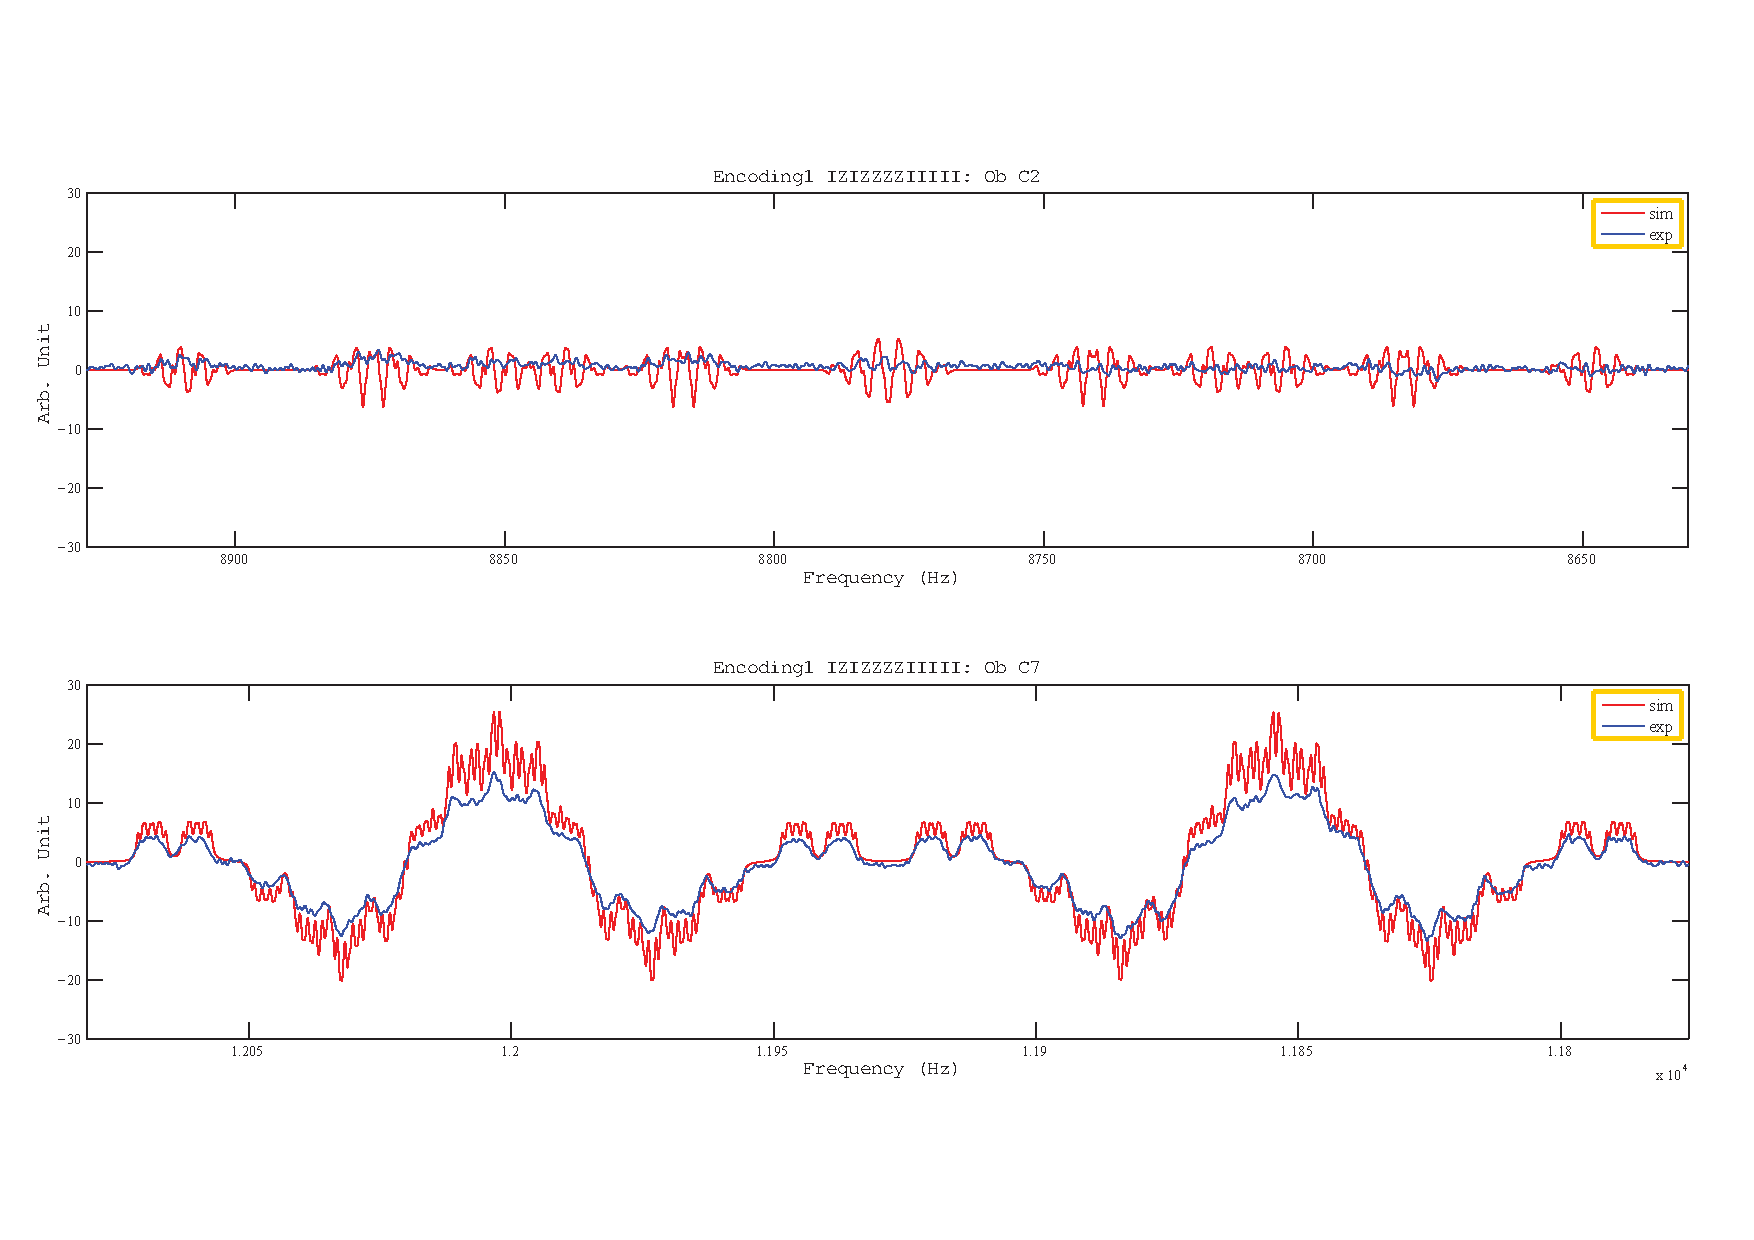
\includegraphics[width=\columnwidth]{Encoding1_without_decouple.pdf}
\end{center}
\setlength{\abovecaptionskip}{-0.35cm}
\caption{\footnotesize{Encoding 1 for C2 and C7 without H decoupled. 10 scans.}}\label{1403and1404}
\end{figure}

\clearpage
Exp 1405: Observe C7 after encoding1 and decouple H. NS=1.\\
Exp 1406: Observe C2 after encoding1 and decouple H. NS=1.\\
\textbf{Note compare with undecoupled experiments, for decoupling experiments I just used 1 scan.}

For C2 the signal is quite close to the 7-qubit case. Good.\\
For C7 the same.

\begin{figure}[htb]
\begin{center}
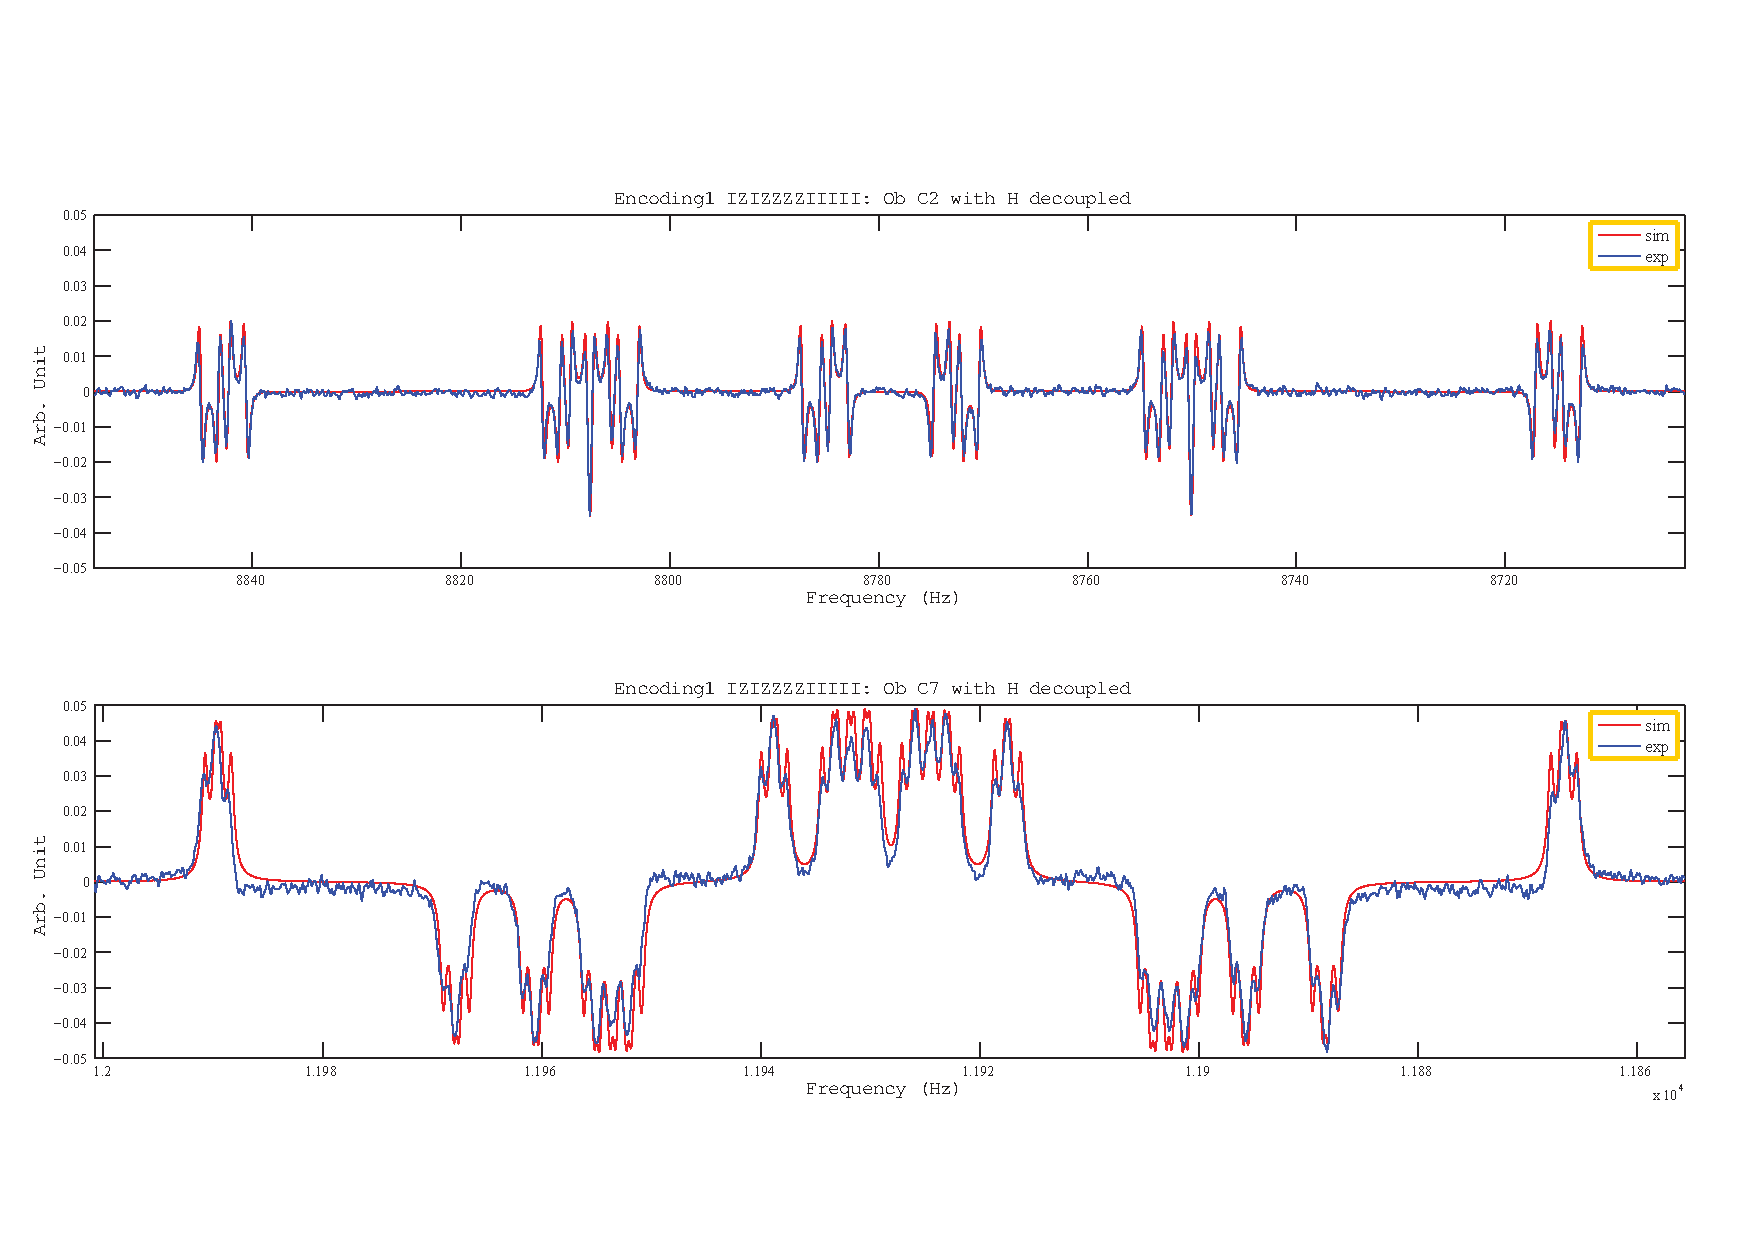
\includegraphics[width=\columnwidth]{Encoding1_with_decouple.pdf}
\end{center}
\setlength{\abovecaptionskip}{-0.35cm}
\caption{\footnotesize{Encoding 1 for C2 and C7 with H decoupled. 1 scan.}}\label{1405and1406}
\end{figure}

\clearpage
Exp 1407: Observe C7 after encoding2. NS=10.\\
Exp 1408: Observe C2 after encoding2. NS=10.\\

For C2 and C7 there are no signals due to the broaden of the C-H couplings.

\begin{figure}[htb]
\begin{center}
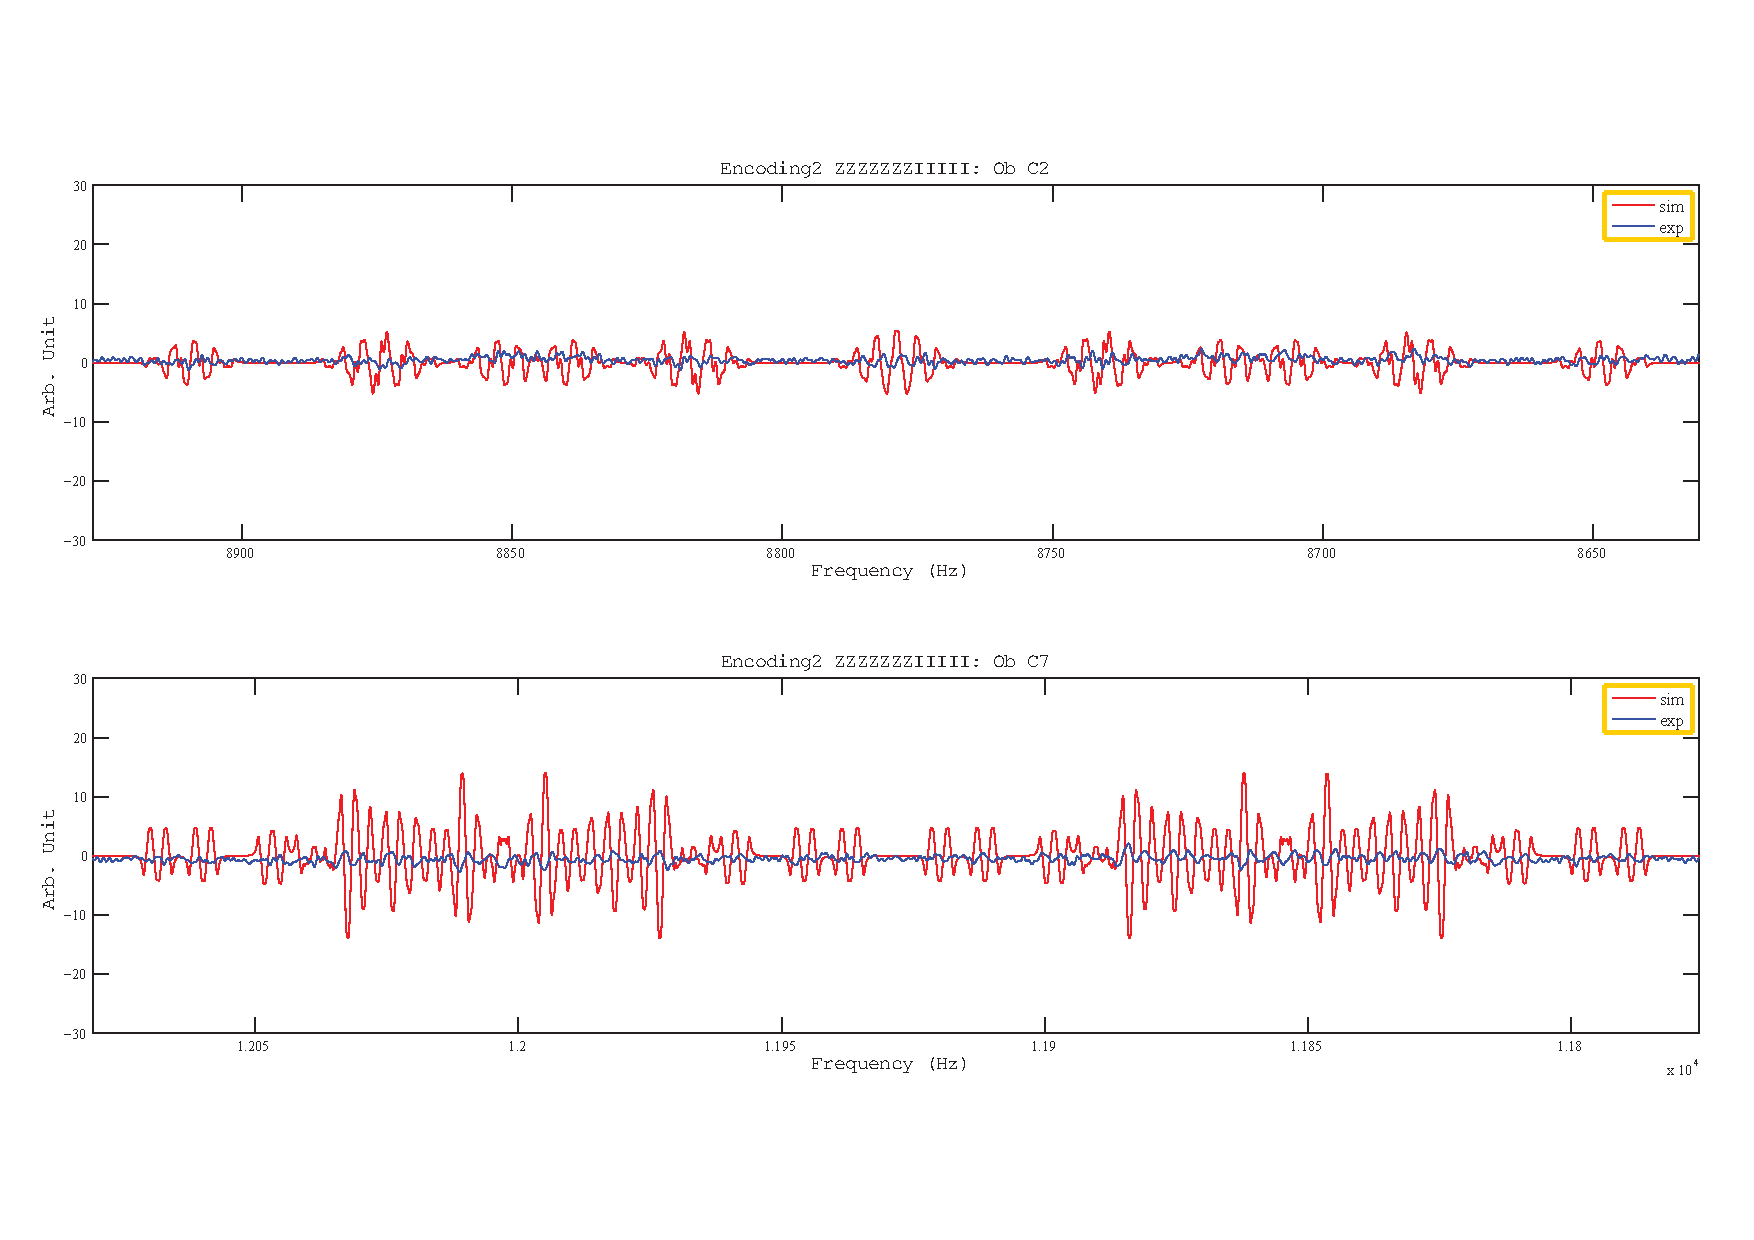
\includegraphics[width=\columnwidth]{Encoding2_without_decouple.pdf}
\end{center}
\setlength{\abovecaptionskip}{-0.35cm}
\caption{\footnotesize{Encoding 2 for C2 and C7 without H decoupled. 10 scans.}}\label{1407and1408}
\end{figure}

\clearpage
Exp 1409: Observe C7 after encoding2 and decouple H. NS=1.\\
Exp 1410: Observe C2 after encoding2 and decouple H. NS=1.\\
\textbf{Note compare with undecoupled experiments, for decoupling experiments I just used 1 scan.}

For C2 and C7 they both look nice.

\begin{figure}[htb]
\begin{center}
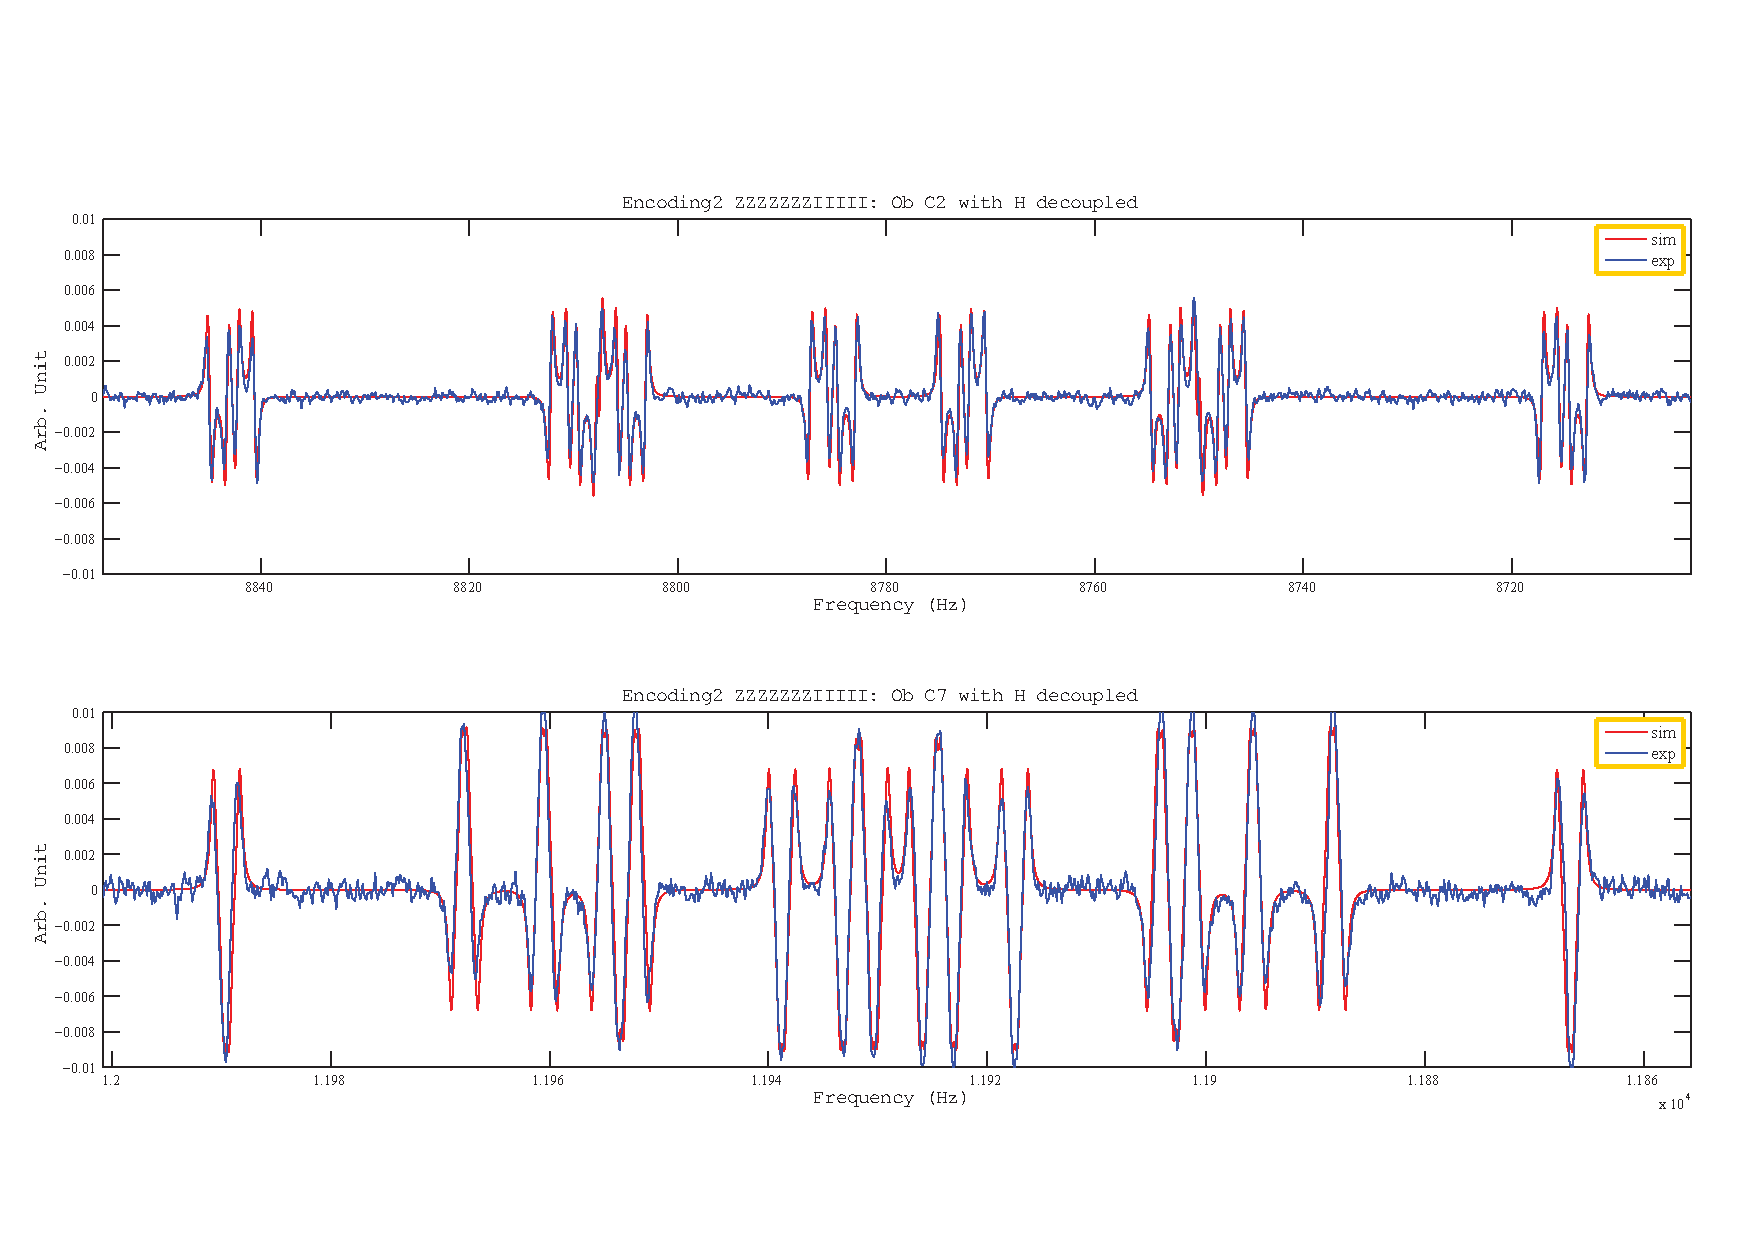
\includegraphics[width=\columnwidth]{Encoding2_with_decouple.pdf}
\end{center}
\setlength{\abovecaptionskip}{-0.35cm}
\caption{\footnotesize{Encoding 2 for C2 and C7 with H decoupled. 1 scan.}}\label{1409and1410}
\end{figure}a

\clearpage
\section{Appendix III: All Pulses for 12 qubits}

The saving folder is '\dir pulseexam\_12qubit\dir C\_rotations\dir'.

$\pi/2$ and $\pi$ rotations on every single spin.
\begin{table}[hbtp]
\begin{tabular} {c||c|c|c|c|c}
  \hline
  Rotation & Length & Fidelity & File & MaxPower C & MaxPower H\\
  \hline
  % after \\: \hline or \cline{col1-col2} \cline{col3-col4} ...
  $R_x^1(\pi/2)$ & 1ms & 0.9981 & twqubit\_C190\_Ufid.mat & 56.0\%, 14000Hz & 22.3\%, 5557Hz\\
  $R_x^2(\pi/2)$ & 1ms & 0.9986 & twqubit\_C290\_Ufid.mat & 41.7\%, 10422Hz & 23.5\%, 5878Hz\\
  $R_x^3(\pi/2)$ & 1ms & 0.9981 & twqubit\_C390\_Ufid.mat & 31.9\%, 7979.0Hz & 22.3\%, 5568Hz\\
  $R_x^4(\pi/2)$ & 1ms & 0.9976 & twqubit\_C490\_Ufid.mat & 31.6\%, 7892.0Hz & 23.8\%, 5954Hz\\
  $R_x^5(\pi/2)$ & 1ms & 0.9981 & twqubit\_C590\_Ufid.mat & 56.1\%, 14033Hz & 30.7\%, 7678Hz\\
  $R_x^6(\pi/2)$ & 1ms & 0.9979 & twqubit\_C690\_Ufid.mat & 57.3\%, 14333Hz & 34.4\%, 8595Hz\\
  $R_x^7(\pi/2)$ & 1ms & 0.9986 & twqubit\_C790\_Ufid.mat & 43.7\%, 10925Hz & 24.8\%, 6207Hz\\
  \hline
  \hline
  $R_x^1(\pi)$ & 2ms & 0.9976 & twqubit\_C1180\_Ufid.mat & 62.6\%, 15655Hz & 34.9\%, 8726Hz\\
  $R_x^2(\pi)$ & 2ms & 0.9980 & twqubit\_C2180\_Ufid.mat & 51.1\%, 12783Hz & 32.4\%, 8094Hz\\
  $R_x^3(\pi)$ & 2ms & 0.9975 & twqubit\_C3180\_Ufid.mat & 37.4\%, 9350.0Hz & 24.0\%, 5997Hz\\
  $R_x^4(\pi)$ & 2ms & 0.9970 & twqubit\_C4180\_Ufid.mat & 45.1\%, 11268Hz & 20.4\%, 5108Hz\\
  $R_x^5(\pi)$ & 2ms & 0.9975 & twqubit\_C5180\_Ufid.mat & 67.6\%, 16895Hz & 31.1\%, 7782Hz\\
  $R_x^6(\pi)$ & 2ms & 0.9976 & twqubit\_C6180\_Ufid.mat & 71.8\%, 17948Hz & 33.6\%, 8396Hz\\
  $R_x^7(\pi)$ & 2ms & 0.9977 & twqubit\_C7180\_Ufid.mat & 51.0\%, 12759Hz & 32.1\%, 8022Hz\\
  \hline
\end{tabular}
\end{table}

Pulses for the encoding part of PPS preparation.
\begin{table}[hbtp]
\begin{tabular} {c||c|c|c|c|c}
  \hline
  Rotation & Length & Fidelity & File & MaxPower C & MaxPower H\\
  \hline
  % after \\: \hline or \cline{col1-col2} \cline{col3-col4} ...
  $R_x^{5,7}(\pi)$ & 2ms & 0.9980 & twqubit\_C57180\_Ufid.mat & 32.3\%, 8072.5Hz & 24.2\%, 6049Hz\\
  $R_x^{2,3}(\pi)$ & 2ms & 0.9978 & twqubit\_C23180\_Ufid.mat & 32.4\%, 8101.5Hz & 22.8\%, 5701Hz\\
  $R_x^{2,3,4,7}(\pi/2)$ & 1ms & 0.9970 & twqubit\_C234790\_Ufid.mat & 37.4\%, 9358.3Hz & 28.9\%, 7213Hz\\
  $R_x^{1,5,6}(\pi)$ & 2ms & 0.9974 & twqubit\_C156180\_Ufid.mat & 32.2\%, 8039.7Hz & 20.3\%, 5086Hz\\
  $R_x^{2,4,7}(\pi/2)R_{-y}^{3}(\pi/2)R_{-z}^{i=2,3,4,7}((w_i-O_1)*3.36\text{ms})$ & 1ms & 0.9964 & twqubit\_C234790withPC\_Ufid.mat & 26.1\%, 6514.5Hz & 20.2\%, 5048Hz\\
  \hline
\end{tabular}
\end{table}

Pulses for polarization crush and phase cycling.
\begin{table}[hbtp]
\begin{tabular} {c||c|c|c|c|c}
  \hline
  Rotation & Length & Fidelity & File & MaxPower C & MaxPower H\\
  \hline
  % after \\: \hline or \cline{col1-col2} \cline{col3-col4} ...
  $R_x^{1-12}(\pi/2)$ & 1ms & 0.9977 & twqubit\_all90\_Ufid.mat & 27.8\%, 6956.6Hz & 30.4\%, 7594Hz\\
  $R_x^{1-6,8-12}(\pi/2)$ & 1ms & 0.9977 & twqubit\_all90butC7\_Ufid.mat & 24.5\%, 6134.9Hz & 25.0\%, 6239Hz\\
  \hline
\end{tabular}
\end{table}

Pulses for the decoding part of PPS preparation.
\begin{table}[!h]
\begin{tabular} {c||c|c|c|c|c}
  \hline
  Rotation & Length & Fidelity & File & MaxPower C & MaxPower H\\
  \hline
  % after \\: \hline or \cline{col1-col2} \cline{col3-col4} ...
  $R_x^{2,3,4,7-12}(\pi)$ & 2ms & 0.9988 & twqubit\_C2347andH180\_Ufid.mat & 61.6\%, 15400Hz & 52.2\%, 13039Hz\\
  $R_x^{1,3,4,6}(\pi/2)R_{-y}^{8-12}(\pi/2)$ & 1ms & 0.9974 & twqubit\_C134690andH90\_Ufid.mat & 24.8\%, 6203.2Hz & 22.1\%, 5529Hz\\
  $R_x^{2,3,4,5,6}(\pi)$ & 2ms & 0.9984 & twqubit\_C23456180\_Ufid.mat & 37.8\%, 9438.2Hz & 23.0\%, 5746Hz\\
  $R_{-y}^{4,6}R_{y}^{1,3}(\pi/2)R_{x}^{2}(\pi/2)R_{-z}^{1}(6.6\text{ms})$ & 1ms & 0.9982 &  twqubit\_C1234690withPC\_Ufid.mat & 28.3\%, 7070.8Hz & 26.9\%, 6717Hz\\
  $R_x^{2,7}(\pi)$ & 2ms & 0.9979 & twqubit\_C27180\_Ufid.mat & 29.1\%, 7285.3Hz & 21.7\%, 5414Hz\\
  $R_{y}^{2}(\pi/2)R_{x}^{5}(\pi/2)$ & 1ms & 0.9975 & twqubit\_C2Y5X90\_Ufid.mat & 28.9\%, 7233.9Hz & 29.2\%, 7292Hz\\
  $R_{x}^{8,9,10,11,12}(\pi/2)$ & 1ms & 0.9982 & twqubit\_H90\_Ufid.mat & 45.6\%, 11405Hz & 27.5\%, 6876Hz\\
  \hline
\end{tabular}
\end{table}

\newpage
All pulses in the saving folder '\dir pulseexam\_12qubit\dir'. The fidelities in the following table are state fidelities
\begin{table}[!h]
\begin{tabular} {c||c|c|c}
  \hline
  Files & Length & Target State & State Fidelity\\
  \hline
  % after \\: \hline or \cline{col1-col2} \cline{col3-col4} ...
  twqubit\_encoding1\_C, H & 32.98ms & IZIZZZZIIIII & 0.9831\\
  twqubit\_encoding2\_C, H & 21.28ms & ZZZZZZZIIIII & 0.9717\\
  twqubit\_encoding3\_C, H & 7.36 ms & ZZZZZZZZZZZZ & 0.9124\\
  twqubit\_phasecycling\_C, H & 1 ms & I$_{+}^{\otimes 12}$ + I$_{-}^{\otimes 12}$ & 0.9125\\
  twqubit\_decoding\_C, H & 68.96 ms & Z$_7\otimes\ket{00000000000}$ & 0.8234\\
  \hline
\end{tabular}
\end{table}

\subsection{New Pulses with 0us Buffer Delay}

Recalculated 18 pulses with 0us buffer. Here is the information.
\begin{table}[!h]
\begin{tabular} {c||c|c|c}
  \hline
  Name & Length & MaxPower C & MaxPower H\\
  \hline
  % after \\: \hline or \cline{col1-col2} \cline{col3-col4} ...
  C790 & 1ms & 46.8\%, 11697Hz & 27.9\%, 6965Hz\\
  C290 & 1ms & 37.8\%, 9456Hz & 25.8\%, 6453Hz\\
  C234790 & 1ms & 39.1\%, 9781Hz & 29.1\%, 7287Hz\\
  C234790withPC & 1ms & 25.1\%, 6286Hz & 20.5\%, 5130Hz\\
  C134690andH90 & 1ms & 27.2\%, 6803Hz & 30.3\%, 7574Hz\\
  C1234690withPC & 1ms & 28.9\%, 7226Hz & 27.3\%, 6819Hz\\
  C2Y5X90 & 1ms & 30.5\%, 7632Hz & 28.8\%, 7212Hz\\
  C590 & 1ms & 61.4\%, 15348Hz & 32.7\%, 8171Hz\\
  C2180 & 2ms & 50.9\%, 12722Hz & 31.4\%, 7859Hz\\
  C6180 & 2ms & 75.2\%, 18790Hz & 33.6\%, 8392Hz\\
  C4180 & 2ms & 47.0\%, 11760Hz & 20.7\%, 5173Hz\\
  C57180 & 2ms & 32.4\%, 8093Hz & 25.4\%, 6361Hz\\
  C1180 & 2ms & 63.0\%, 15747Hz & 35.0\%, 8744Hz\\
  C23180 & 2ms & 34.2\%, 8540Hz & 23.3\%, 5827Hz\\
  C156180 & 2ms & 31.6\%, 7899Hz & 20.7\%, 5183Hz\\
  C2347180andH180 & 2ms & 62.2\%, 15555Hz & 52.0\%, 13011Hz\\
  C23456180 & 2ms & 38.0\%, 9497Hz & 23.2\%, 5791Hz\\
  C27180 & 2ms & 28.7\%, 7176Hz & 21.5\%, 5380Hz\\
  \hline
\end{tabular}
\end{table} 
\clearpage
\section{Appendix II: Important Figures and Experimental Spectra}

\begin{figure}[htb]
\begin{center}
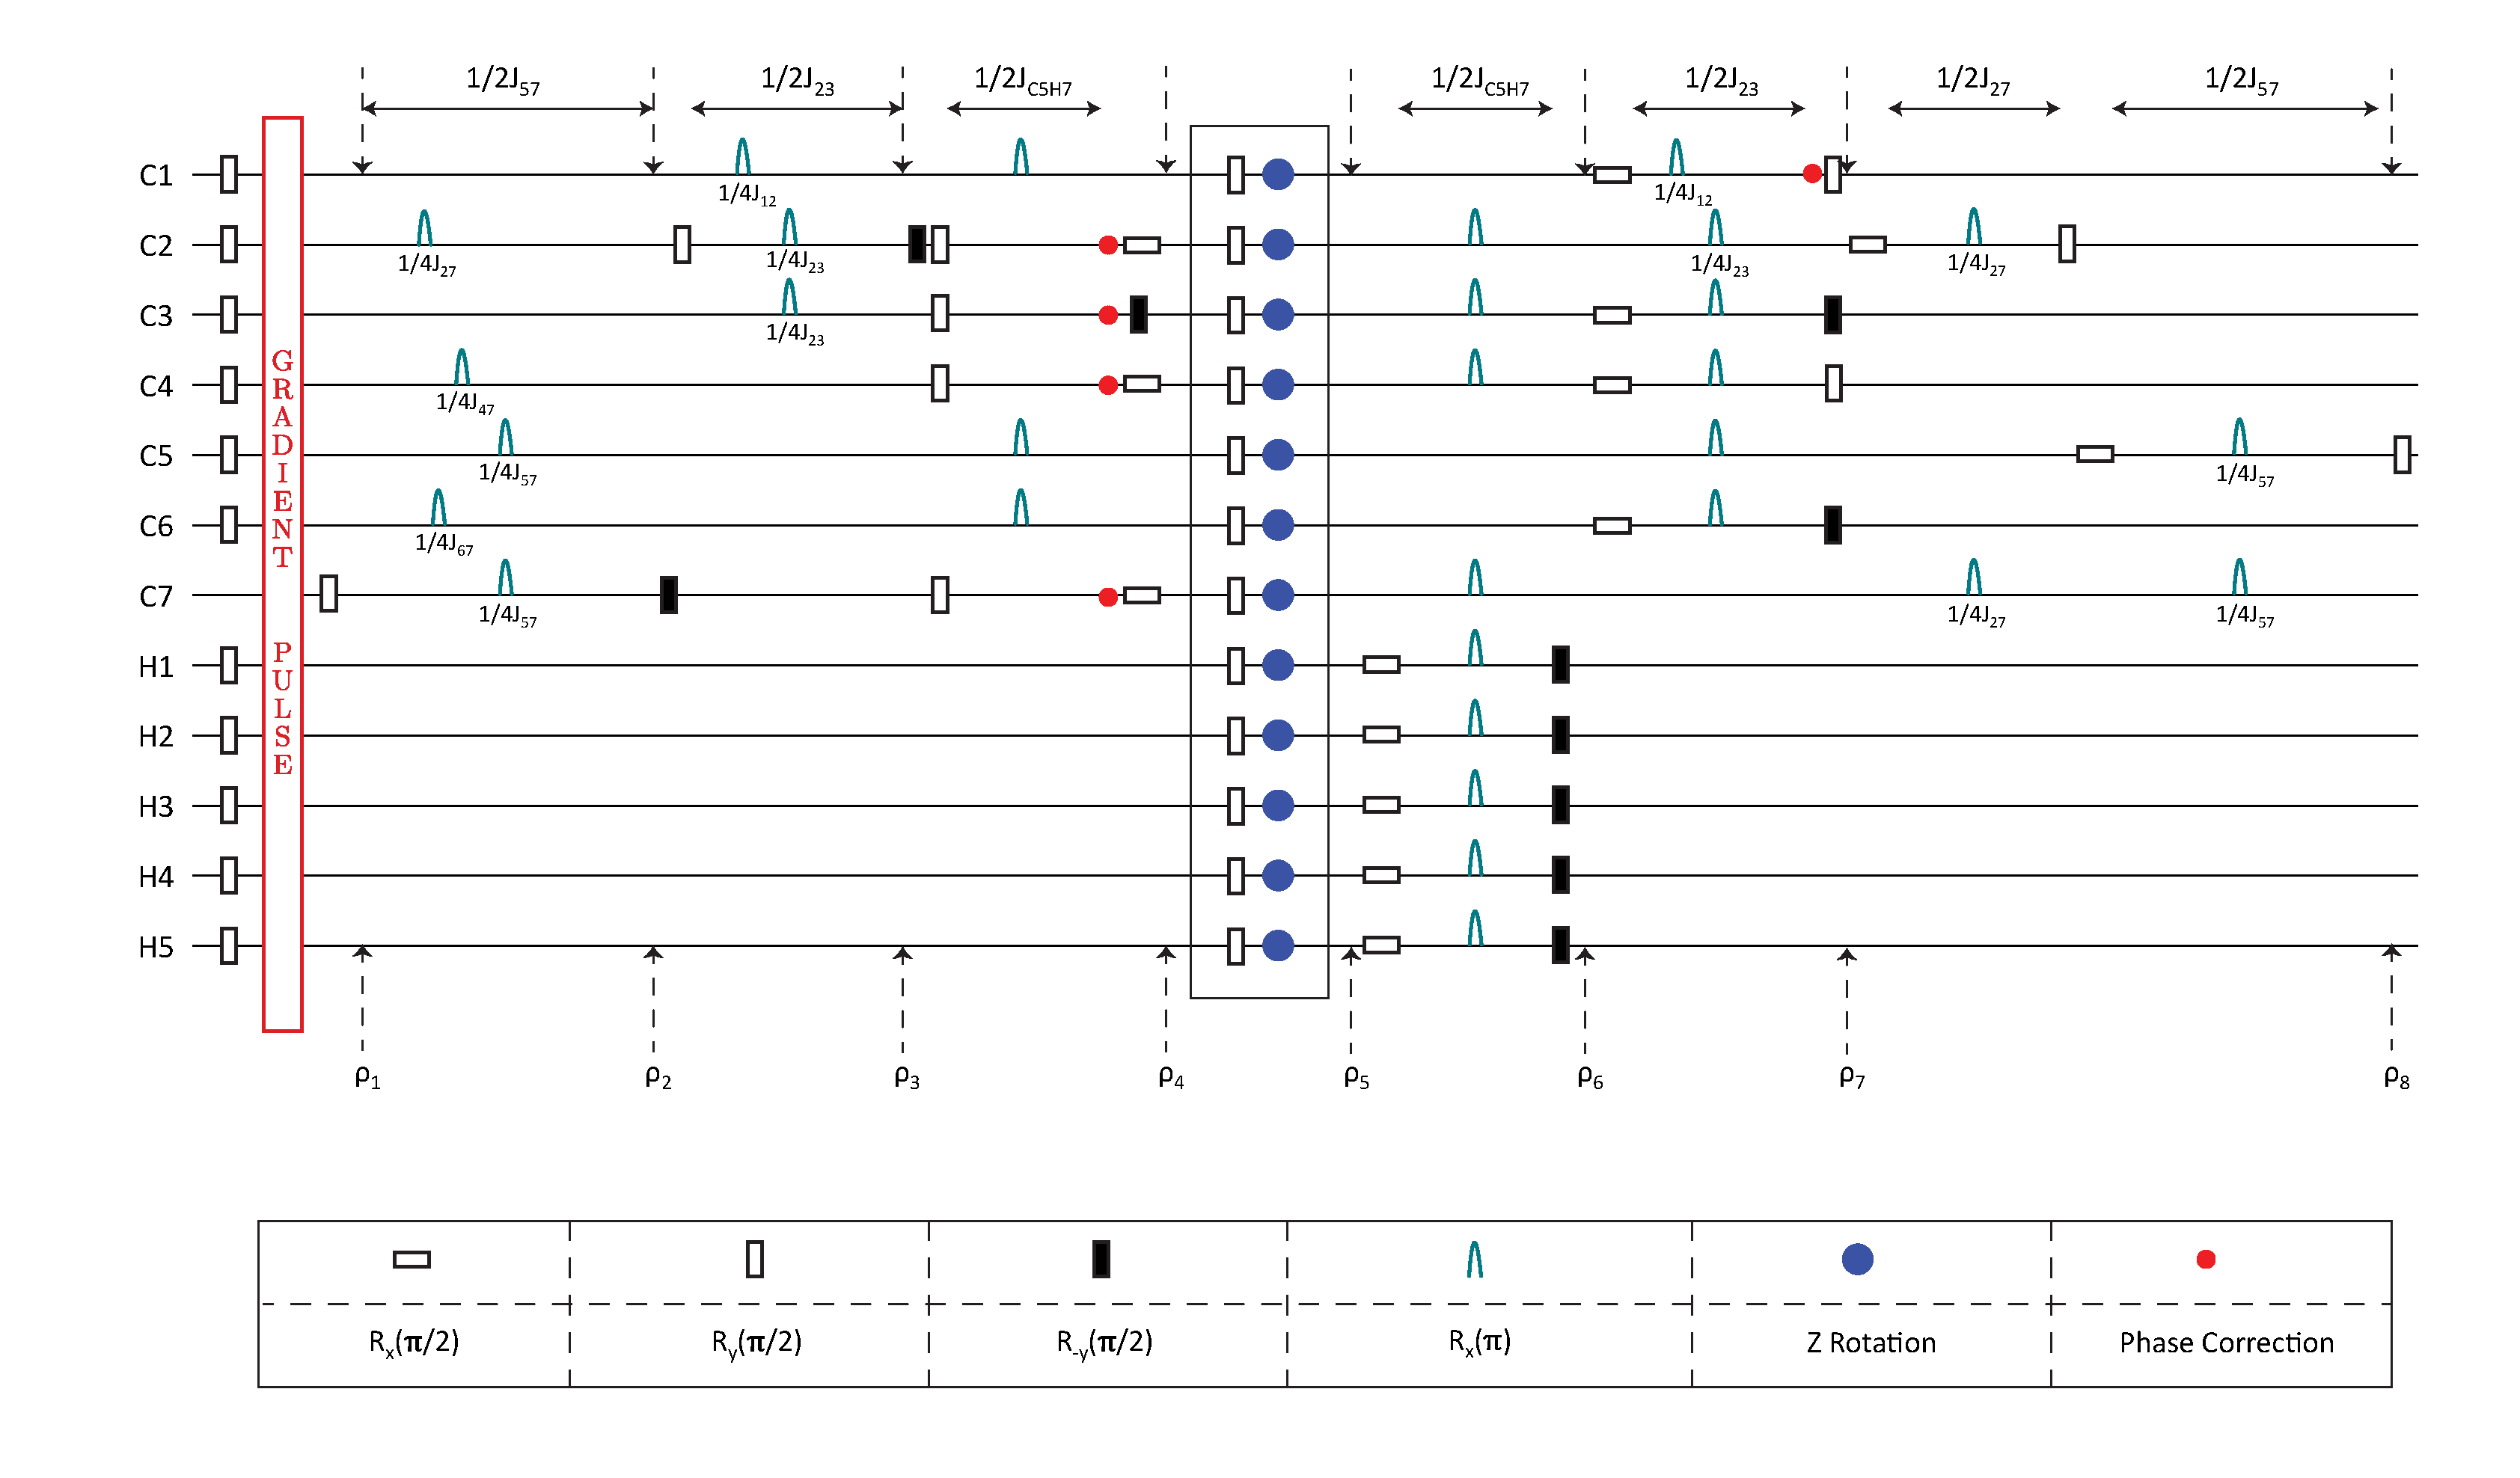
\includegraphics[width=\columnwidth]{12-spin-pps-circuit.pdf}
\end{center}
\setlength{\abovecaptionskip}{-0.35cm}
\caption{\footnotesize{Circuit to realize the 12-qubit PPS with some simplifications.}}\label{12-spin-pps-circuit}
\end{figure}

\begin{figure}[htb]
\begin{center}
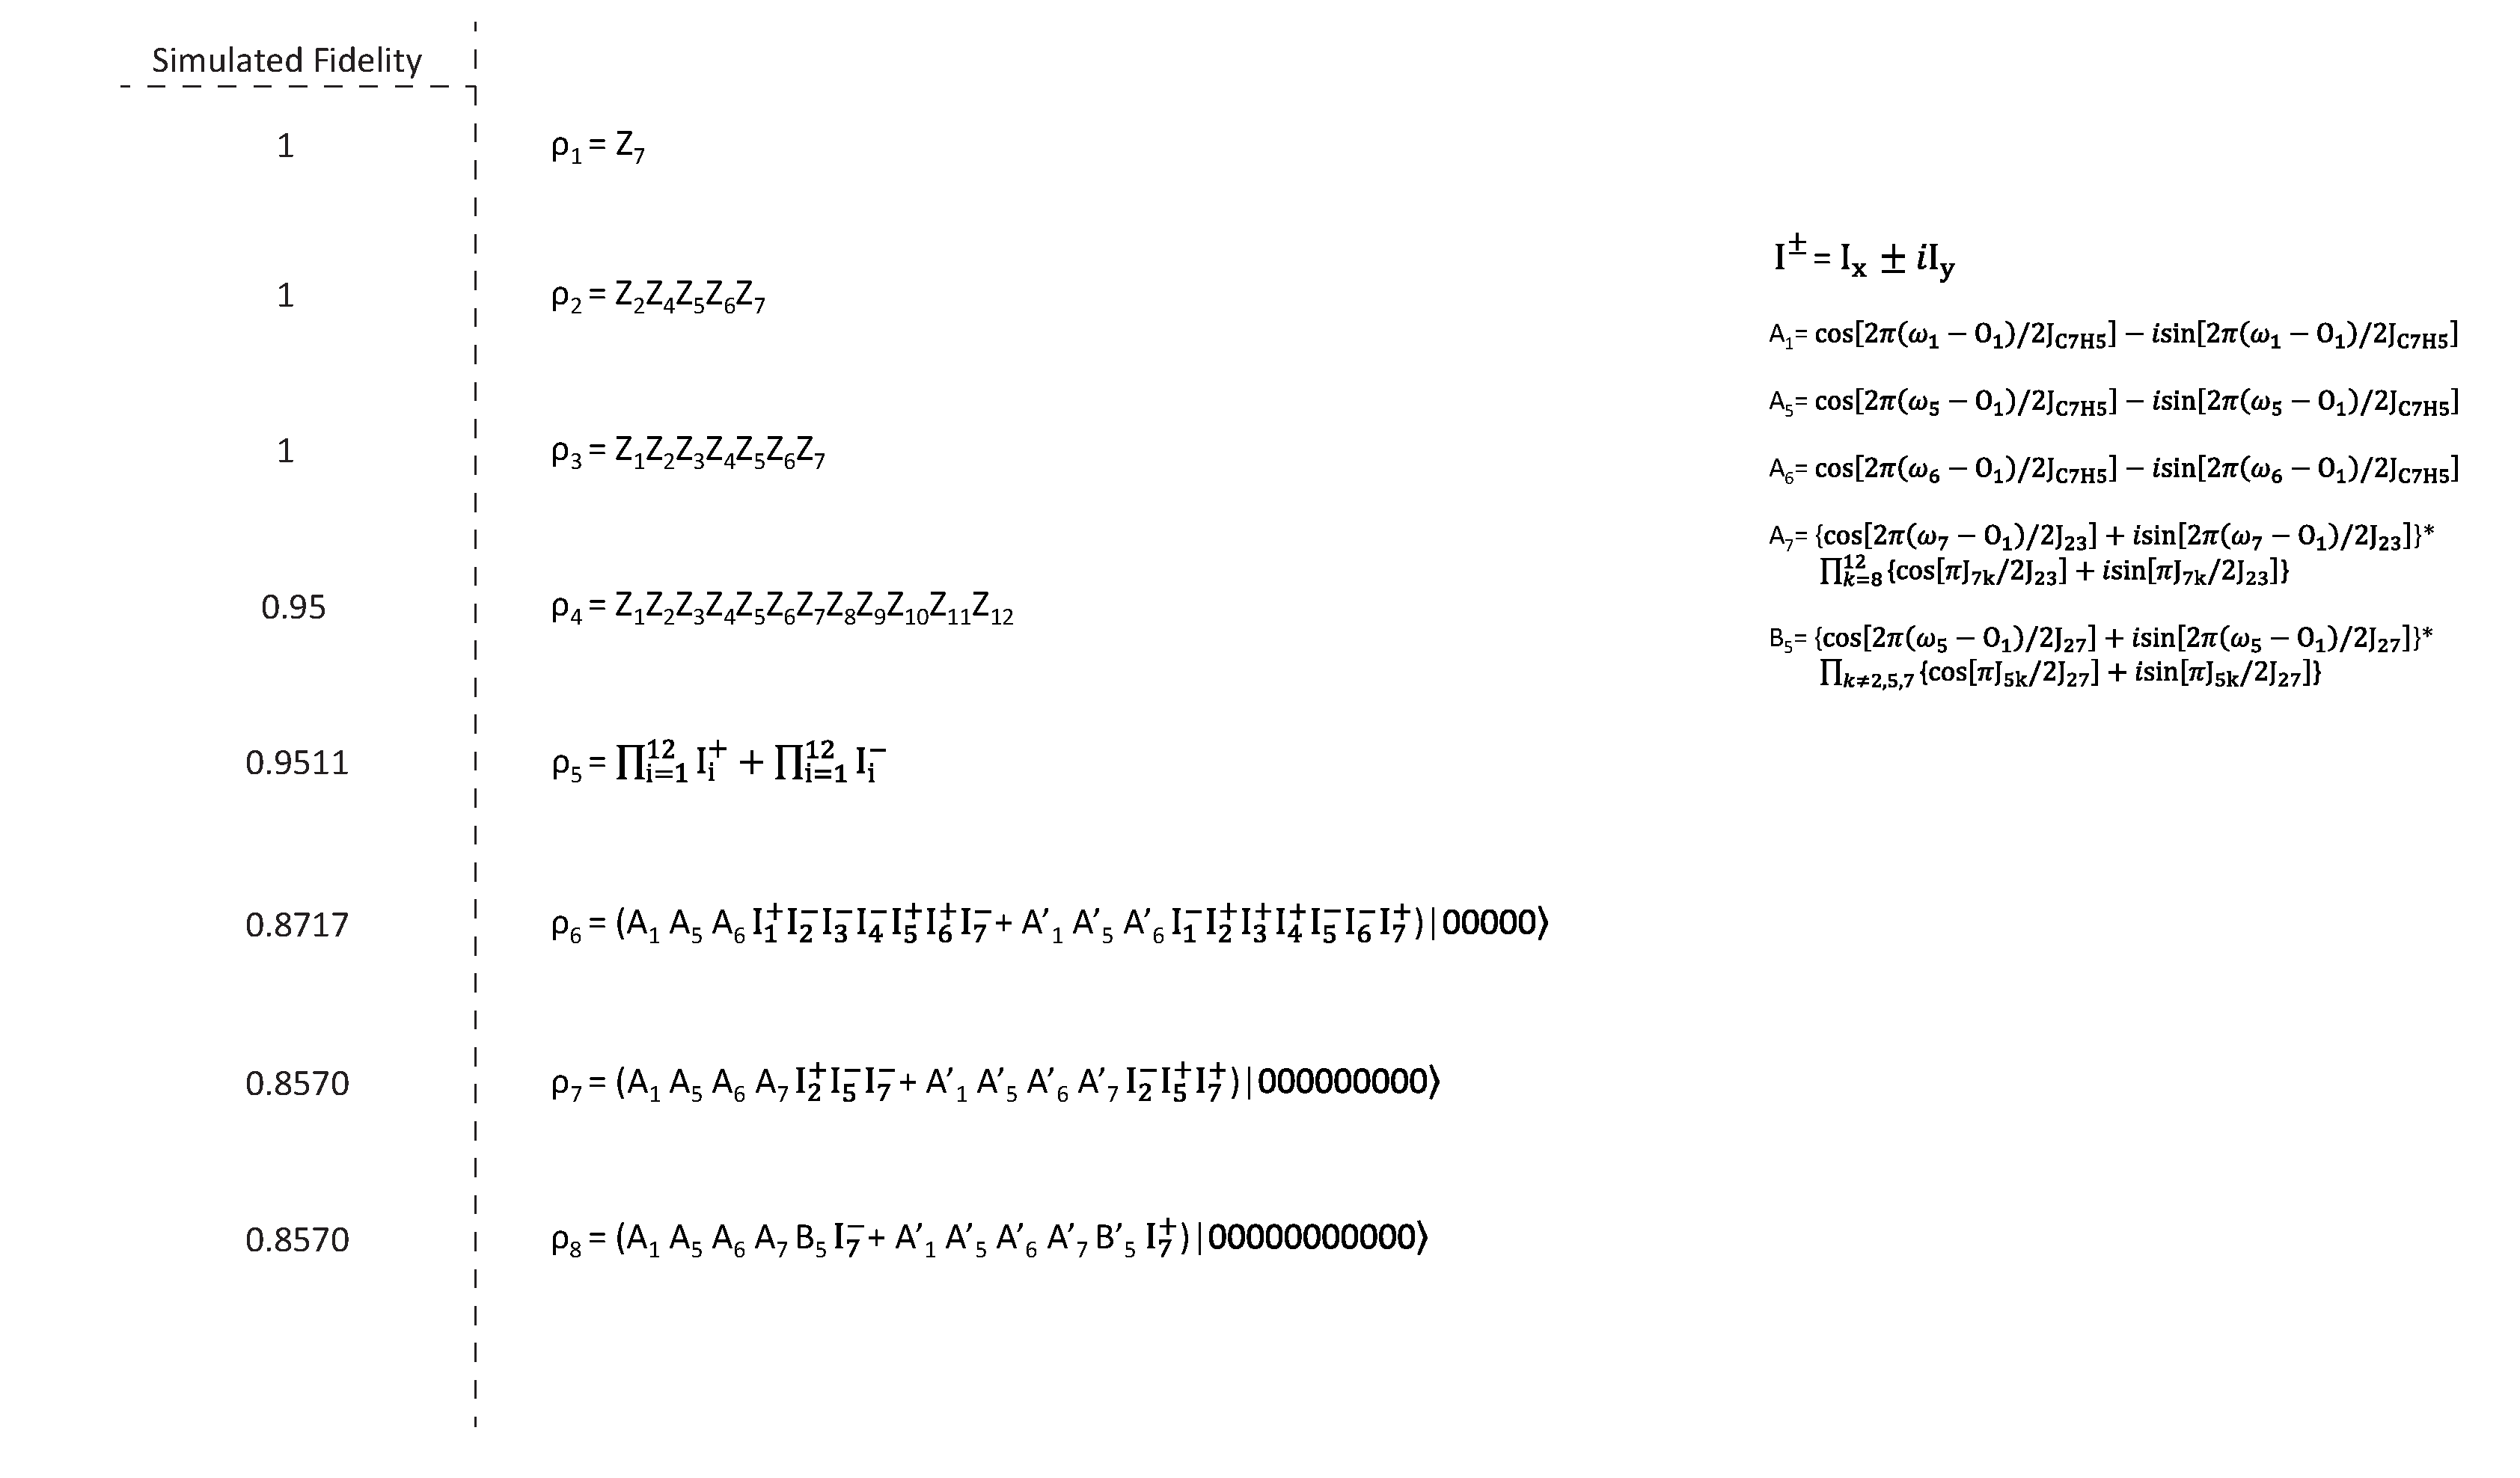
\includegraphics[width=\columnwidth]{circuit-simulation-result.pdf}
\end{center}
\setlength{\abovecaptionskip}{-0.35cm}
\caption{\footnotesize{States and fidelities after every step in the 12-qubit PPS circuit.}}\label{circuit-simulation-result}
\end{figure}

\clearpage
Exp 1401: Observe C7 by GRAPE as the reference. NS=10.\\
Exp 1402: Observe C2 by GRAPE as the reference. NS=10. \\

\begin{figure}[htb]
\begin{center}
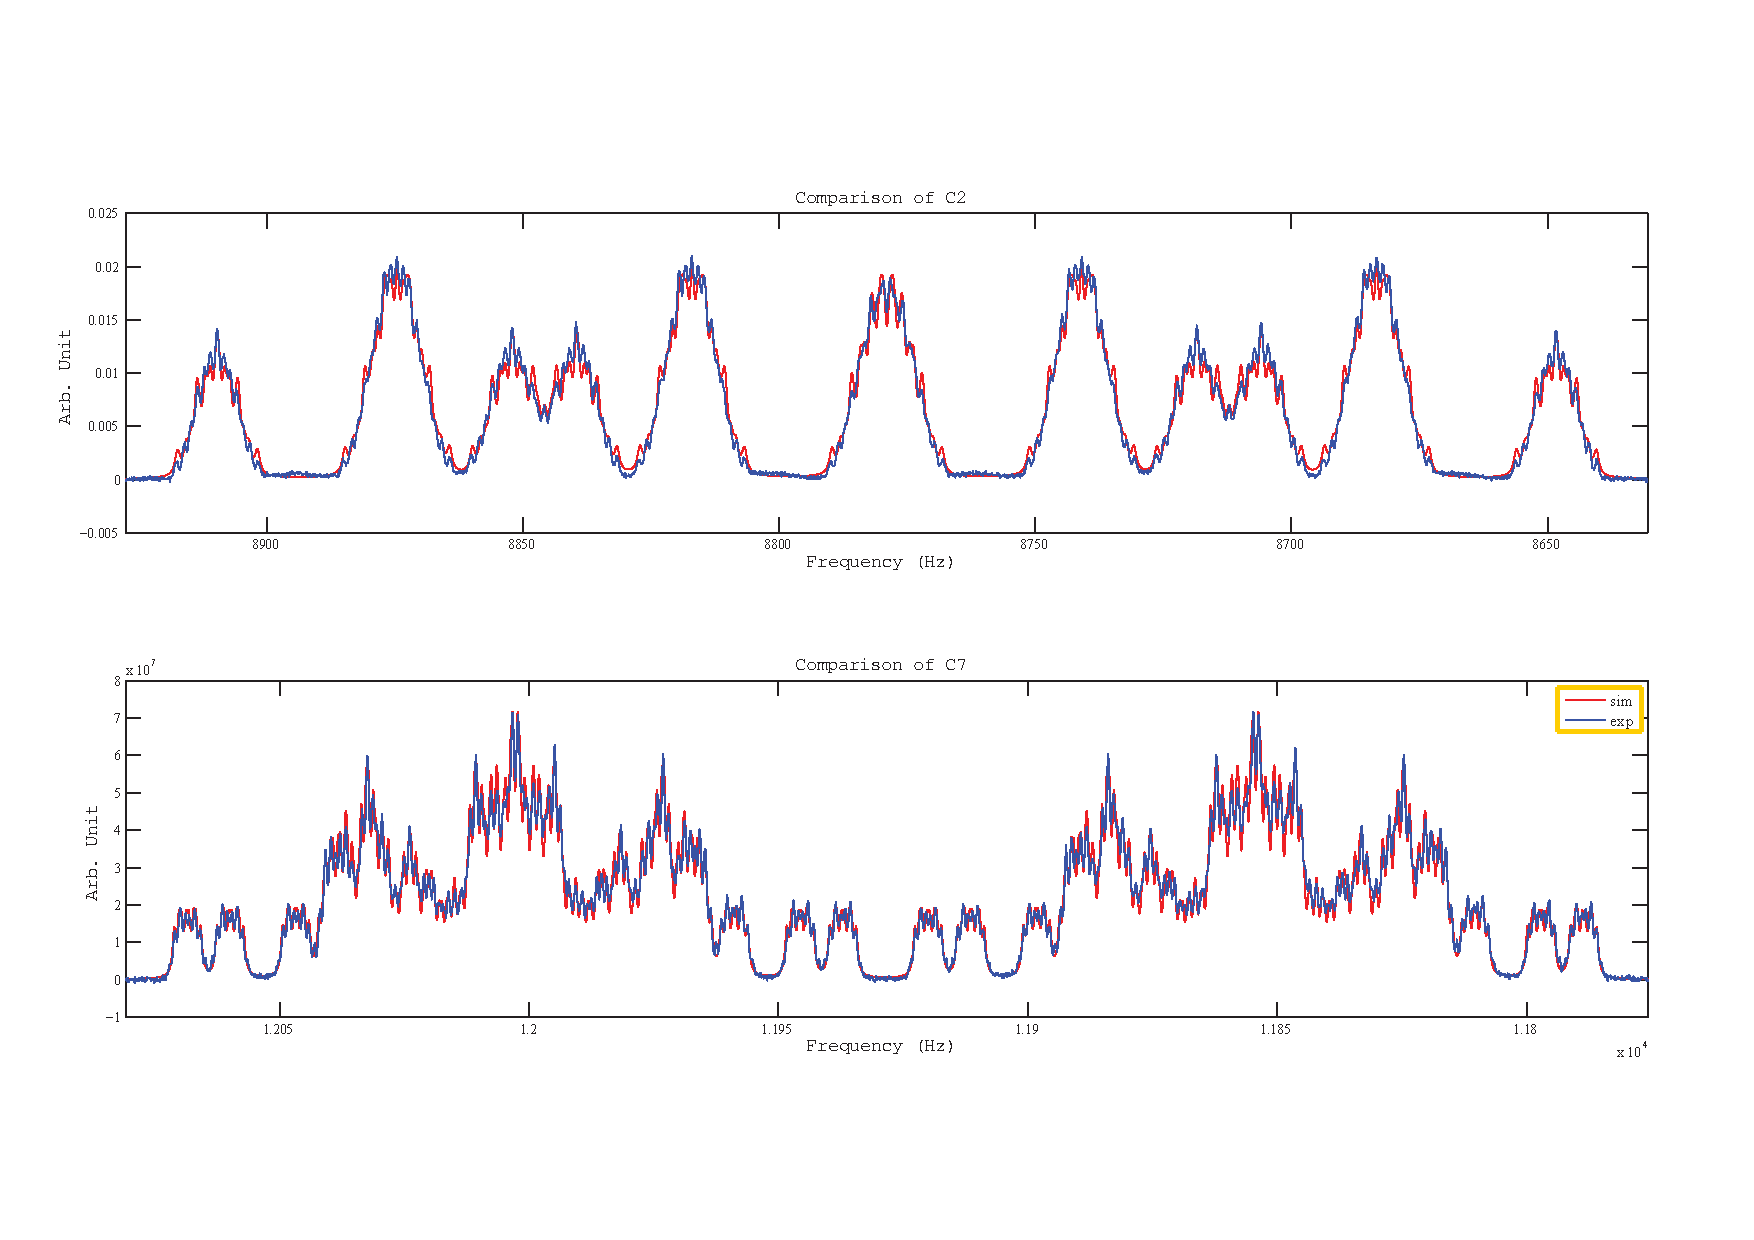
\includegraphics[width=\columnwidth]{Thermal_C2andC7.pdf}
\end{center}
\setlength{\abovecaptionskip}{-0.35cm}
\caption{\footnotesize{Comparison of the thermal for C2 and C7. Blue is experiment and Red is the simulation by the fitted Hamiltonian.}}\label{1401and1402}
\end{figure}

\clearpage
Exp 1403: Observe C7 after encoding1. NS=10.\\
Exp 1404: Observe C2 after encoding1. NS=10.\\

For C2 there is no signal because for Z24567 some couplings are close to 0 and the C2-H couplings broadens the peak. So for 12 qubits, these small couplings cannot be resolved.\\
For C7 it matches well with the simulation. However, the small couplings are annihilated due to the C7-H couplings too.

\begin{figure}[htb]
\begin{center}
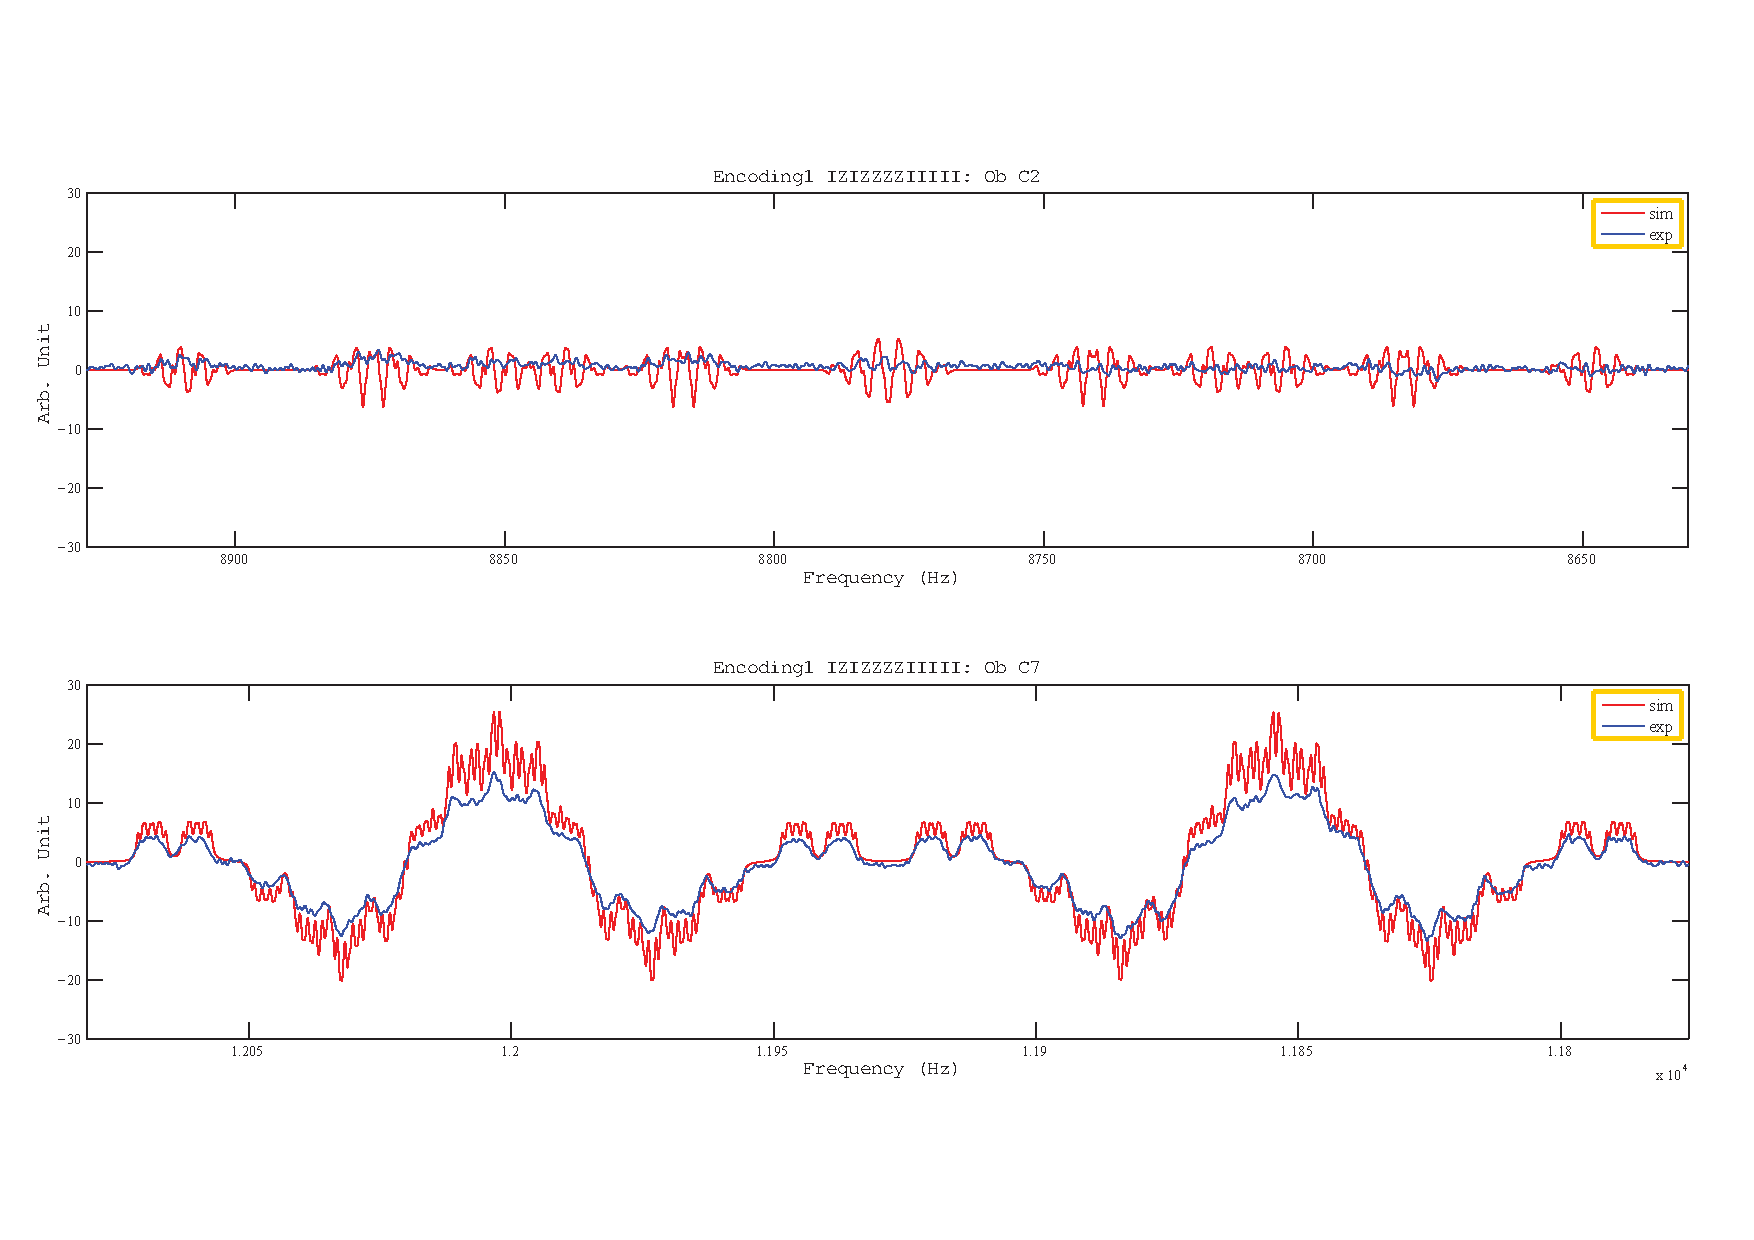
\includegraphics[width=\columnwidth]{Encoding1_without_decouple.pdf}
\end{center}
\setlength{\abovecaptionskip}{-0.35cm}
\caption{\footnotesize{Encoding 1 for C2 and C7 without H decoupled. 10 scans.}}\label{1403and1404}
\end{figure}

\clearpage
Exp 1405: Observe C7 after encoding1 and decouple H. NS=1.\\
Exp 1406: Observe C2 after encoding1 and decouple H. NS=1.\\
\textbf{Note compare with undecoupled experiments, for decoupling experiments I just used 1 scan.}

For C2 the signal is quite close to the 7-qubit case. Good.\\
For C7 the same.

\begin{figure}[htb]
\begin{center}
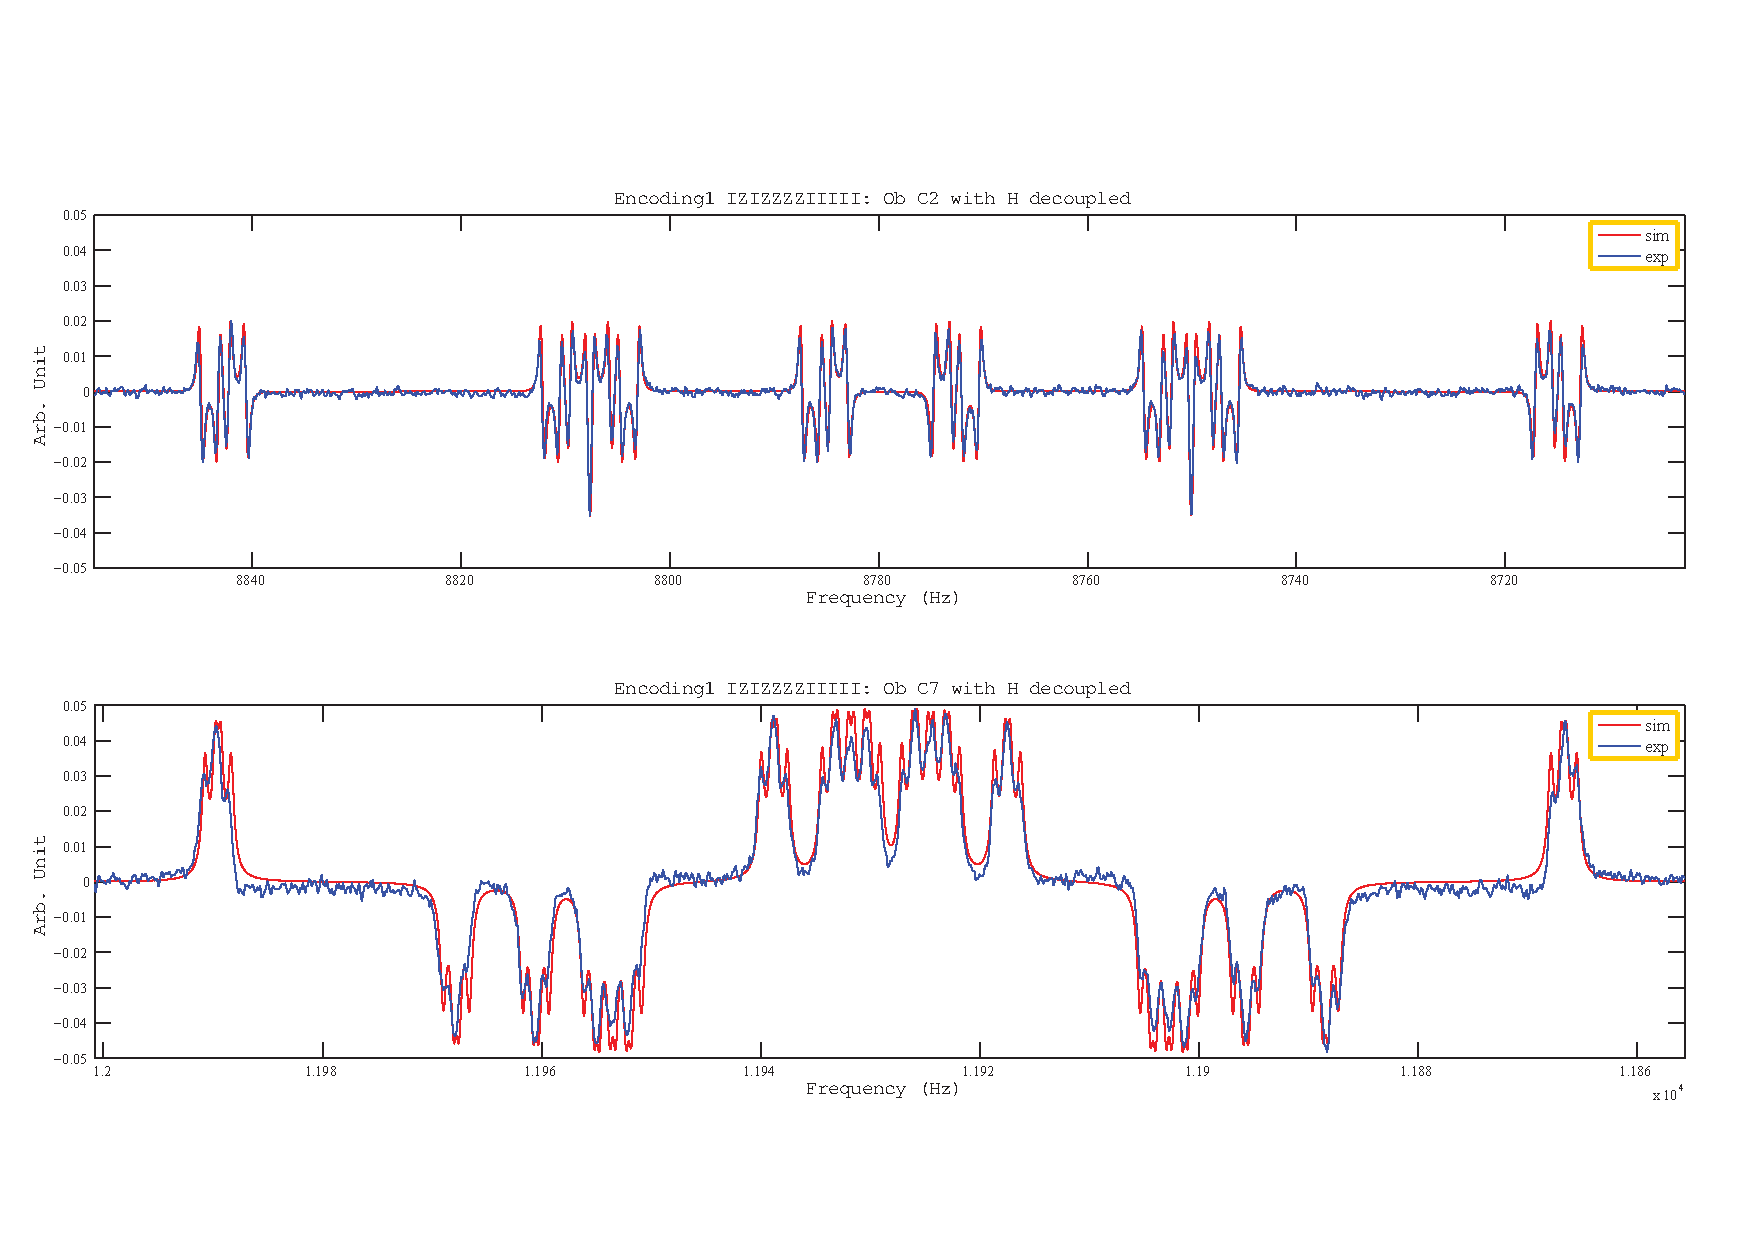
\includegraphics[width=\columnwidth]{Encoding1_with_decouple.pdf}
\end{center}
\setlength{\abovecaptionskip}{-0.35cm}
\caption{\footnotesize{Encoding 1 for C2 and C7 with H decoupled. 1 scan.}}\label{1405and1406}
\end{figure}

\clearpage
Exp 1407: Observe C7 after encoding2. NS=10.\\
Exp 1408: Observe C2 after encoding2. NS=10.\\

For C2 and C7 there are no signals due to the broaden of the C-H couplings.

\begin{figure}[htb]
\begin{center}
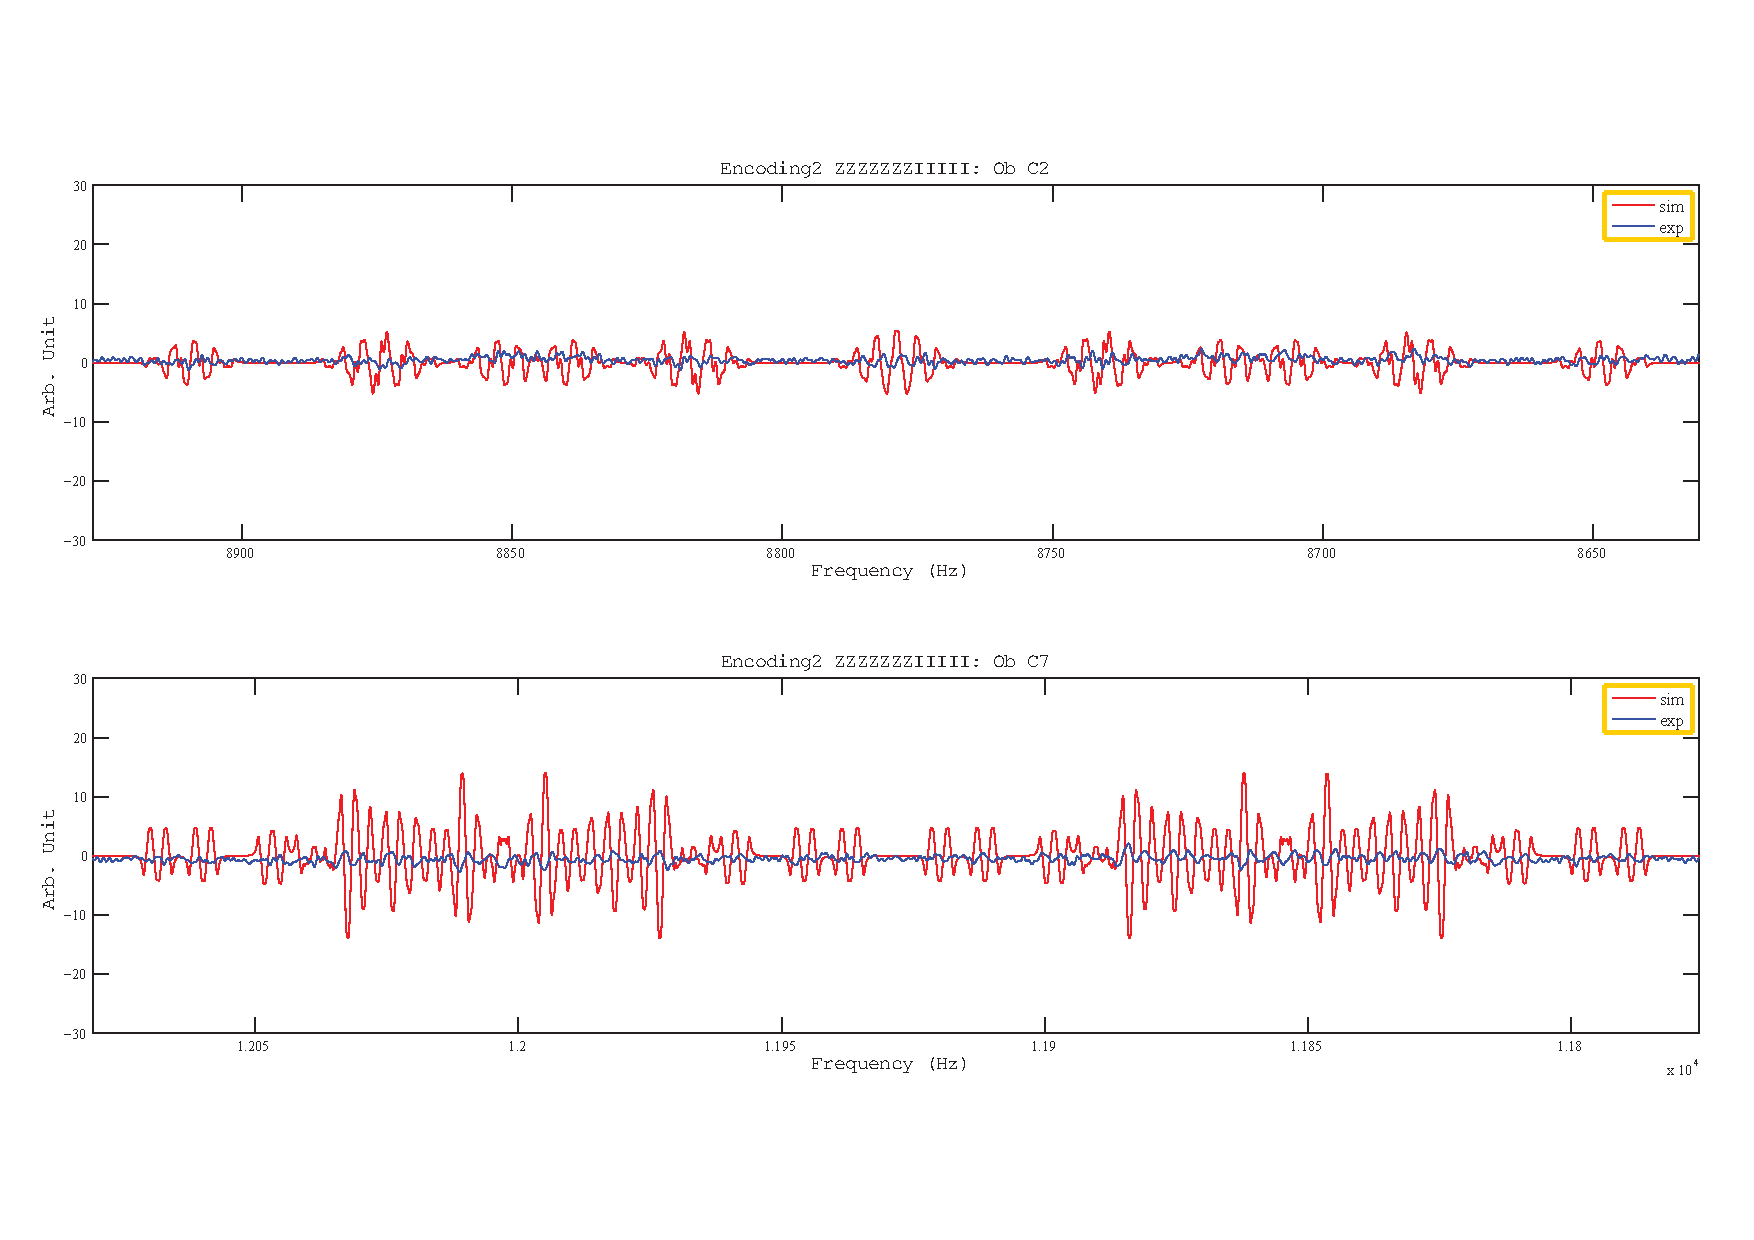
\includegraphics[width=\columnwidth]{Encoding2_without_decouple.pdf}
\end{center}
\setlength{\abovecaptionskip}{-0.35cm}
\caption{\footnotesize{Encoding 2 for C2 and C7 without H decoupled. 10 scans.}}\label{1407and1408}
\end{figure}

\clearpage
Exp 1409: Observe C7 after encoding2 and decouple H. NS=1.\\
Exp 1410: Observe C2 after encoding2 and decouple H. NS=1.\\
\textbf{Note compare with undecoupled experiments, for decoupling experiments I just used 1 scan.}

For C2 and C7 they both look nice.

\begin{figure}[htb]
\begin{center}
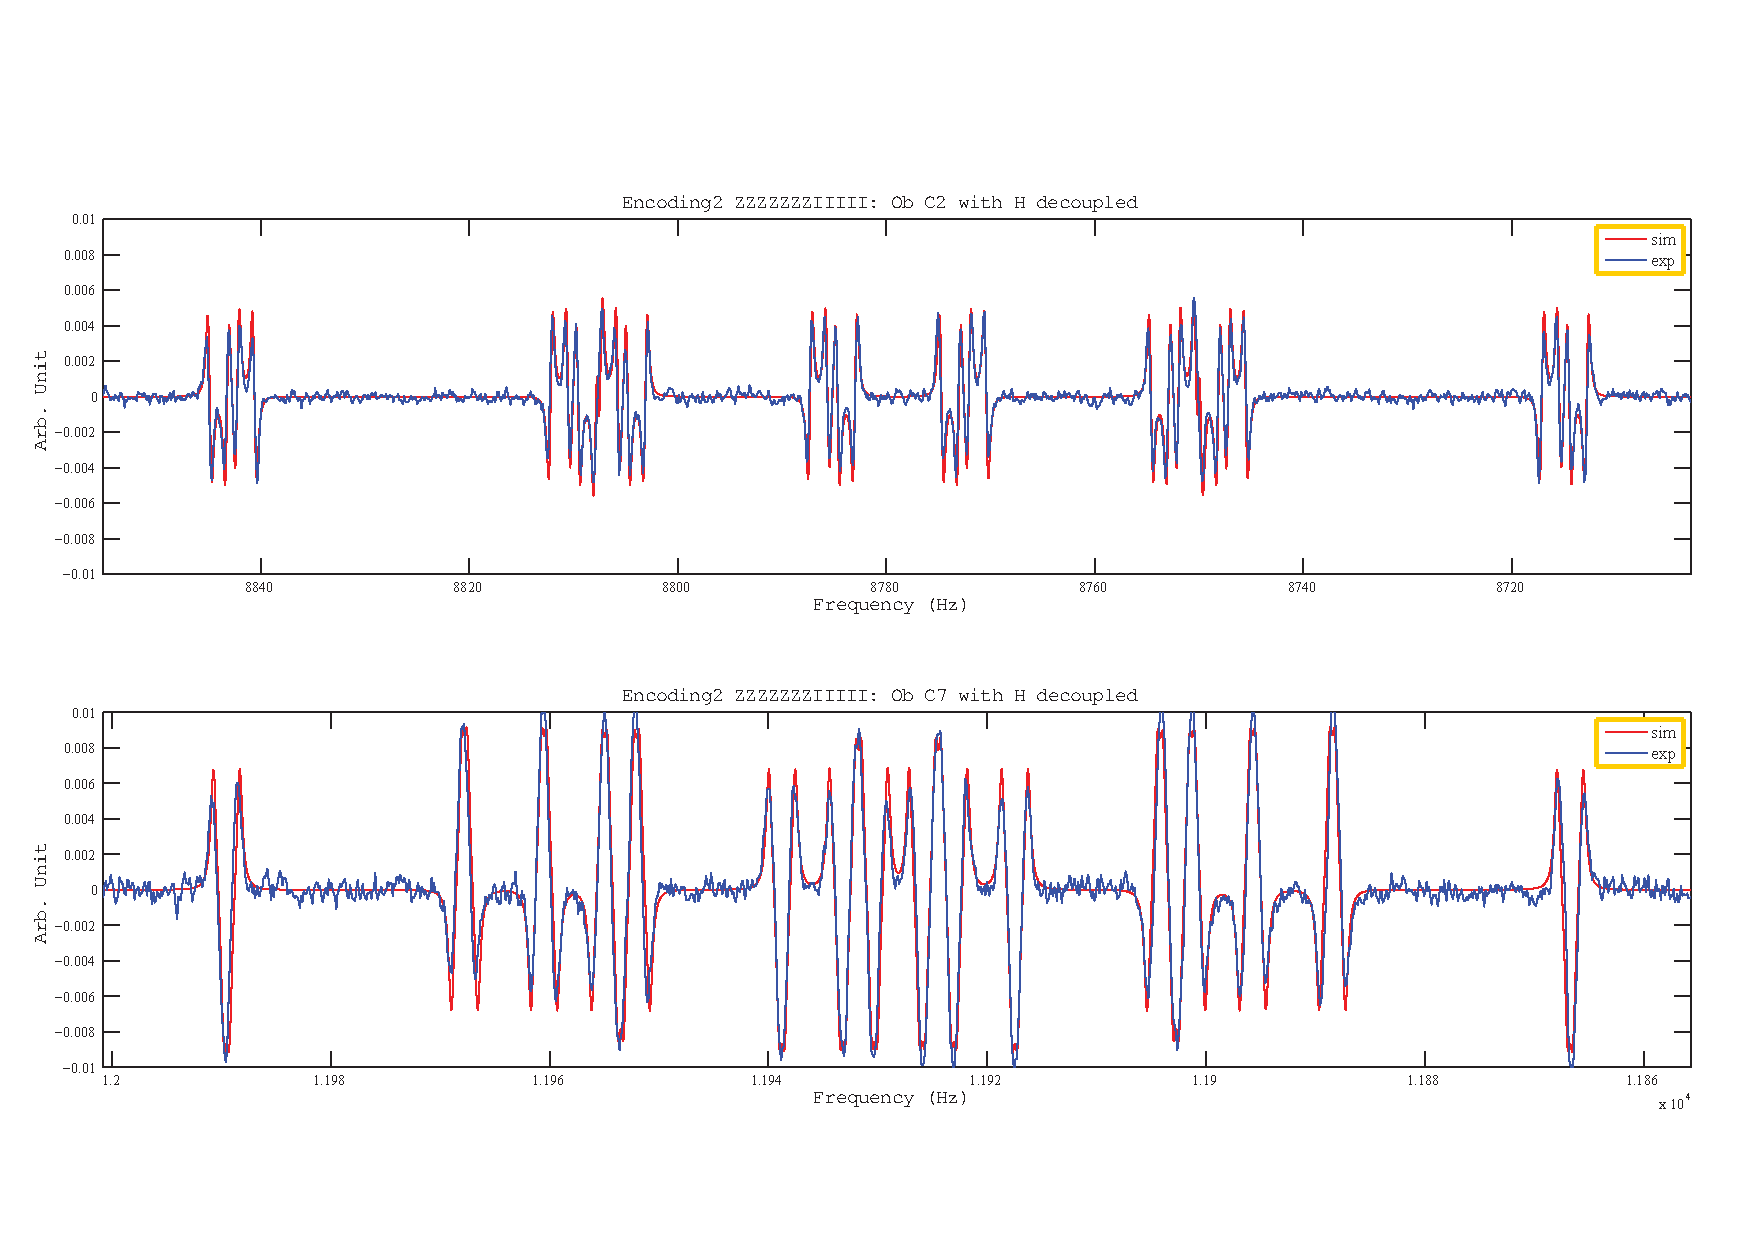
\includegraphics[width=\columnwidth]{Encoding2_with_decouple.pdf}
\end{center}
\setlength{\abovecaptionskip}{-0.35cm}
\caption{\footnotesize{Encoding 2 for C2 and C7 with H decoupled. 1 scan.}}\label{1409and1410}
\end{figure}

\clearpage
Exp 1411: Observe C7 after encoding3. Encoding 3 is applied on thermal. NS=1.\\
Exp 1412: Observe C2 after encoding3. Encoding 3 is applied on thermal. NS=1.\\
\textbf{Note the encoding 3 operator is just applied on thermal because if it is applied consequently after encoding 2 the spectra has no signal.}

They look okay as I did not adjust the experimental parameters much. In principal, only C-H will be anti-phase.

\begin{figure}[htb]
\begin{center}
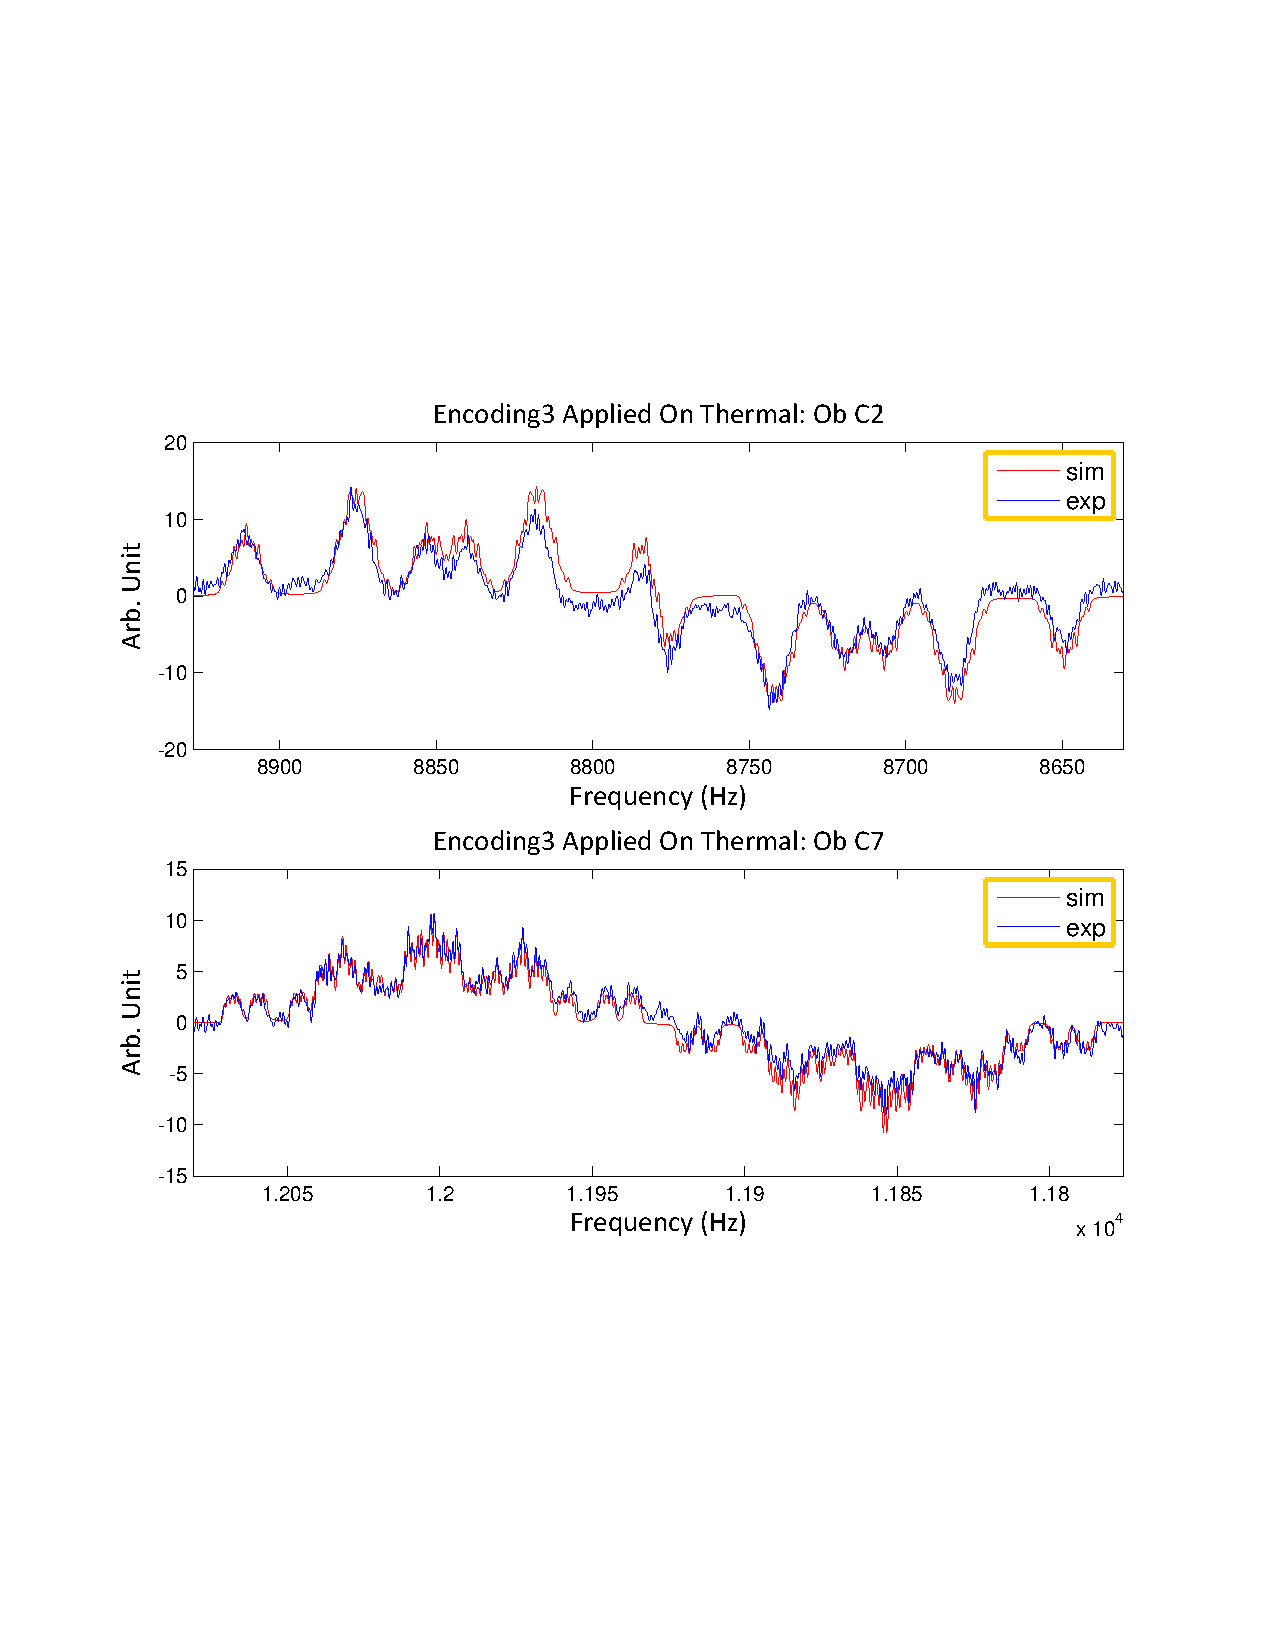
\includegraphics[width=\columnwidth]{Encoding3_without_decouple.pdf}
\end{center}
\setlength{\abovecaptionskip}{-0.35cm}
\caption{\footnotesize{Encoding 3 for C2 and C7 applied on thermal. 1 scan.}}\label{1411and1412}
\end{figure}
\clearpage
\section{Appendix III: All Pulses for 12 qubits}

The saving folder is '\dir pulseexam\_12qubit\dir C\_rotations\dir'.

$\pi/2$ and $\pi$ rotations on every single spin.
\begin{table}[hbtp]
\begin{tabular} {c||c|c|c|c|c}
  \hline
  Rotation & Length & Fidelity & File & MaxPower C & MaxPower H\\
  \hline
  % after \\: \hline or \cline{col1-col2} \cline{col3-col4} ...
  $R_x^1(\pi/2)$ & 1ms & 0.9981 & twqubit\_C190\_Ufid.mat & 56.0\%, 14000Hz & 22.3\%, 5557Hz\\
  $R_x^2(\pi/2)$ & 1ms & 0.9986 & twqubit\_C290\_Ufid.mat & 41.7\%, 10422Hz & 23.5\%, 5878Hz\\
  $R_x^3(\pi/2)$ & 1ms & 0.9981 & twqubit\_C390\_Ufid.mat & 31.9\%, 7979.0Hz & 22.3\%, 5568Hz\\
  $R_x^4(\pi/2)$ & 1ms & 0.9976 & twqubit\_C490\_Ufid.mat & 31.6\%, 7892.0Hz & 23.8\%, 5954Hz\\
  $R_x^5(\pi/2)$ & 1ms & 0.9981 & twqubit\_C590\_Ufid.mat & 56.1\%, 14033Hz & 30.7\%, 7678Hz\\
  $R_x^6(\pi/2)$ & 1ms & 0.9979 & twqubit\_C690\_Ufid.mat & 57.3\%, 14333Hz & 34.4\%, 8595Hz\\
  $R_x^7(\pi/2)$ & 1ms & 0.9986 & twqubit\_C790\_Ufid.mat & 43.7\%, 10925Hz & 24.8\%, 6207Hz\\
  \hline
  \hline
  $R_x^1(\pi)$ & 2ms & 0.9976 & twqubit\_C1180\_Ufid.mat & 62.6\%, 15655Hz & 34.9\%, 8726Hz\\
  $R_x^2(\pi)$ & 2ms & 0.9980 & twqubit\_C2180\_Ufid.mat & 51.1\%, 12783Hz & 32.4\%, 8094Hz\\
  $R_x^3(\pi)$ & 2ms & 0.9975 & twqubit\_C3180\_Ufid.mat & 37.4\%, 9350.0Hz & 24.0\%, 5997Hz\\
  $R_x^4(\pi)$ & 2ms & 0.9970 & twqubit\_C4180\_Ufid.mat & 45.1\%, 11268Hz & 20.4\%, 5108Hz\\
  $R_x^5(\pi)$ & 2ms & 0.9975 & twqubit\_C5180\_Ufid.mat & 67.6\%, 16895Hz & 31.1\%, 7782Hz\\
  $R_x^6(\pi)$ & 2ms & 0.9976 & twqubit\_C6180\_Ufid.mat & 71.8\%, 17948Hz & 33.6\%, 8396Hz\\
  $R_x^7(\pi)$ & 2ms & 0.9977 & twqubit\_C7180\_Ufid.mat & 51.0\%, 12759Hz & 32.1\%, 8022Hz\\
  \hline
\end{tabular}
\end{table}

Pulses for the encoding part of PPS preparation.
\begin{table}[hbtp]
\begin{tabular} {c||c|c|c|c|c}
  \hline
  Rotation & Length & Fidelity & File & MaxPower C & MaxPower H\\
  \hline
  % after \\: \hline or \cline{col1-col2} \cline{col3-col4} ...
  $R_x^{5,7}(\pi)$ & 2ms & 0.9980 & twqubit\_C57180\_Ufid.mat & 32.3\%, 8072.5Hz & 24.2\%, 6049Hz\\
  $R_x^{2,3}(\pi)$ & 2ms & 0.9978 & twqubit\_C23180\_Ufid.mat & 32.4\%, 8101.5Hz & 22.8\%, 5701Hz\\
  $R_x^{2,3,4,7}(\pi/2)$ & 1ms & 0.9970 & twqubit\_C234790\_Ufid.mat & 37.4\%, 9358.3Hz & 28.9\%, 7213Hz\\
  $R_x^{1,5,6}(\pi)$ & 2ms & 0.9974 & twqubit\_C156180\_Ufid.mat & 32.2\%, 8039.7Hz & 20.3\%, 5086Hz\\
  $R_x^{2,4,7}(\pi/2)R_{-y}^{3}(\pi/2)R_{-z}^{i=2,3,4,7}((w_i-O_1)*3.36\text{ms})$ & 1ms & 0.9964 & twqubit\_C234790withPC\_Ufid.mat & 26.1\%, 6514.5Hz & 20.2\%, 5048Hz\\
  \hline
\end{tabular}
\end{table}

Pulses for polarization crush and phase cycling.
\begin{table}[hbtp]
\begin{tabular} {c||c|c|c|c|c}
  \hline
  Rotation & Length & Fidelity & File & MaxPower C & MaxPower H\\
  \hline
  % after \\: \hline or \cline{col1-col2} \cline{col3-col4} ...
  $R_x^{1-12}(\pi/2)$ & 1ms & 0.9977 & twqubit\_all90\_Ufid.mat & 27.8\%, 6956.6Hz & 30.4\%, 7594Hz\\
  $R_x^{1-6,8-12}(\pi/2)$ & 1ms & 0.9977 & twqubit\_all90butC7\_Ufid.mat & 24.5\%, 6134.9Hz & 25.0\%, 6239Hz\\
  \hline
\end{tabular}
\end{table}

Pulses for the decoding part of PPS preparation.
\begin{table}[!h]
\begin{tabular} {c||c|c|c|c|c}
  \hline
  Rotation & Length & Fidelity & File & MaxPower C & MaxPower H\\
  \hline
  % after \\: \hline or \cline{col1-col2} \cline{col3-col4} ...
  $R_x^{2,3,4,7-12}(\pi)$ & 2ms & 0.9988 & twqubit\_C2347andH180\_Ufid.mat & 61.6\%, 15400Hz & 52.2\%, 13039Hz\\
  $R_x^{1,3,4,6}(\pi/2)R_{-y}^{8-12}(\pi/2)$ & 1ms & 0.9974 & twqubit\_C134690andH90\_Ufid.mat & 24.8\%, 6203.2Hz & 22.1\%, 5529Hz\\
  $R_x^{2,3,4,5,6}(\pi)$ & 2ms & 0.9984 & twqubit\_C23456180\_Ufid.mat & 37.8\%, 9438.2Hz & 23.0\%, 5746Hz\\
  $R_{-y}^{4,6}R_{y}^{1,3}(\pi/2)R_{x}^{2}(\pi/2)R_{-z}^{1}(6.6\text{ms})$ & 1ms & 0.9982 &  twqubit\_C1234690withPC\_Ufid.mat & 28.3\%, 7070.8Hz & 26.9\%, 6717Hz\\
  $R_x^{2,7}(\pi)$ & 2ms & 0.9979 & twqubit\_C27180\_Ufid.mat & 29.1\%, 7285.3Hz & 21.7\%, 5414Hz\\
  $R_{y}^{2}(\pi/2)R_{x}^{5}(\pi/2)$ & 1ms & 0.9975 & twqubit\_C2Y5X90\_Ufid.mat & 28.9\%, 7233.9Hz & 29.2\%, 7292Hz\\
  $R_{x}^{8,9,10,11,12}(\pi/2)$ & 1ms & 0.9982 & twqubit\_H90\_Ufid.mat & 45.6\%, 11405Hz & 27.5\%, 6876Hz\\
  \hline
\end{tabular}
\end{table}

\newpage
All pulses in the saving folder '\dir pulseexam\_12qubit\dir'. The fidelities in the following table are state fidelities
\begin{table}[!h]
\begin{tabular} {c||c|c|c}
  \hline
  Files & Length & Target State & State Fidelity\\
  \hline
  % after \\: \hline or \cline{col1-col2} \cline{col3-col4} ...
  twqubit\_encoding1\_C, H & 32.98ms & IZIZZZZIIIII & 0.9831\\
  twqubit\_encoding2\_C, H & 21.28ms & ZZZZZZZIIIII & 0.9717\\
  twqubit\_encoding3\_C, H & 7.36 ms & ZZZZZZZZZZZZ & 0.9124\\
  twqubit\_phasecycling\_C, H & 1 ms & I$_{+}^{\otimes 12}$ + I$_{-}^{\otimes 12}$ & 0.9125\\
  twqubit\_decoding\_C, H & 68.96 ms & Z$_7\otimes\ket{00000000000}$ & 0.8234\\
  \hline
\end{tabular}
\end{table}

\subsection{New Pulses with 0us Buffer Delay}

Recalculated 18 pulses with 0us buffer. Here is the information.
\begin{table}[!h]
\begin{tabular} {c||c|c|c}
  \hline
  Name & Length & MaxPower C & MaxPower H\\
  \hline
  % after \\: \hline or \cline{col1-col2} \cline{col3-col4} ...
  C790 & 1ms & 46.8\%, 11697Hz & 27.9\%, 6965Hz\\
  C290 & 1ms & 37.8\%, 9456Hz & 25.8\%, 6453Hz\\
  C234790 & 1ms & 39.1\%, 9781Hz & 29.1\%, 7287Hz\\
  C234790withPC & 1ms & 25.1\%, 6286Hz & 20.5\%, 5130Hz\\
  C134690andH90 & 1ms & 27.2\%, 6803Hz & 30.3\%, 7574Hz\\
  C1234690withPC & 1ms & 28.9\%, 7226Hz & 27.3\%, 6819Hz\\
  C2Y5X90 & 1ms & 30.5\%, 7632Hz & 28.8\%, 7212Hz\\
  C590 & 1ms & 61.4\%, 15348Hz & 32.7\%, 8171Hz\\
  C2180 & 2ms & 50.9\%, 12722Hz & 31.4\%, 7859Hz\\
  C6180 & 2ms & 75.2\%, 18790Hz & 33.6\%, 8392Hz\\
  C4180 & 2ms & 47.0\%, 11760Hz & 20.7\%, 5173Hz\\
  C57180 & 2ms & 32.4\%, 8093Hz & 25.4\%, 6361Hz\\
  C1180 & 2ms & 63.0\%, 15747Hz & 35.0\%, 8744Hz\\
  C23180 & 2ms & 34.2\%, 8540Hz & 23.3\%, 5827Hz\\
  C156180 & 2ms & 31.6\%, 7899Hz & 20.7\%, 5183Hz\\
  C2347180andH180 & 2ms & 62.2\%, 15555Hz & 52.0\%, 13011Hz\\
  C23456180 & 2ms & 38.0\%, 9497Hz & 23.2\%, 5791Hz\\
  C27180 & 2ms & 28.7\%, 7176Hz & 21.5\%, 5380Hz\\
  \hline
\end{tabular}
\end{table} 

\begin{thebibliography}{99}
%\bibitem{Moussa2012} O. Moussa, M. da Silva, C. Ryan, and R. Laflamme, Phys. Rev. Lett. \textbf{109}, 070504 (2012).

\end{thebibliography}


\end{document}
